\documentclass[a4paper, 11pt, oneside, BCOR=0mm, DIV=15]{scrbook} %a4paper; landscape

%\documentclass[a4paper, 11pt, oneside, BCOR=0mm, DIV=15]{scrbook}

\usepackage{lmodern}
\usepackage[T1]{fontenc}
\usepackage[utf8]{inputenc}
%\usepackage[latin1]{inputenc}
\usepackage[francais]{babel}
\usepackage{scrpage2}
\usepackage{amsthm}
\usepackage{amsmath}
\usepackage{amssymb}
\usepackage{amsfonts}
\usepackage{latexsym}
\usepackage[calcwidth]{titlesec}
\usepackage[titles]{tocloft}
\usepackage{color}
\usepackage{setspace}
\usepackage{framed}
\usepackage{graphicx}
\usepackage{enumitem}
\usepackage{mdwlist}
\usepackage{multicol, lipsum}
\usepackage{eurosym}
\usepackage{ifthen}
\usepackage{tkz-euclide}
\usetkzobj{all}
\usepackage{tikz}
\usepackage{tabularx}
\usepackage{array}
\usepackage[pdfborder={0 0 0}]{hyperref}
\usepackage{stmaryrd}
\usepackage{mathrsfs}
\usepackage{pdflscape}
%\usepackage[thinlines]{easytable}
%\usepackage{pst-plot}
%\usepackage{mathtools}
\usepackage{multirow}

%---------------------Jeff
\usepackage{textcomp}
\usepackage{tasks}
\usepackage{ragged2e}
\usepackage{xargs}
\usepackage{pgfplots}
\pgfplotsset{compat=1.11}

\usepackage{icomma}
\usepackage{systeme}
\sysautonum{(*)}

\usetikzlibrary{arrows, shadows, positioning}
\usetikzlibrary{external}
\usetikzlibrary{calc}
\usetikzlibrary{shapes.geometric}
\usetikzlibrary{fit}
\usetikzlibrary{arrows.meta}


% Faarwen défineiren
\def\scriptcolor{navy}
\definecolor{webgreen}{rgb}{0, 0.5, 0} % less intense green
\definecolor{webblue}{rgb}{0, 0, 0.5} % less intense blue
\definecolor{webred}{rgb}{0.5, 0, 0} % less intense red                                                        
\definecolor{lightslategray}{RGB}{119, 136, 153}
\definecolor{darkslategray}{RGB}{47, 79, 79}
\definecolor{steelblue}{RGB}{70, 130, 180}
%\definecolor{midnightblue}{RGB}{25, 25, 112}
\definecolor{darkcyan}{RGB}{0, 139, 139}
%\definecolor{lightseagreen}{RGB}{32,  178, 170}
%\definecolor{aqua}{RGB}{0, 255, 255}
\definecolor{turquoise}{RGB}{0, 206, 209}
%\definecolor{cadetblue}{RGB}{95, 158, 160}
\definecolor{blueviolet}{RGB}{138, 43, 226}
%\definecolor{darkviolet}{RGB}{148, 0, 211}
\definecolor{navy}{RGB}{0, 0, 128}
\definecolor{royalblue}{RGB}{65, 105, 225}
\definecolor{skyblue}{RGB}{135, 206, 250}
\definecolor{slateblue}{RGB}{106, 90, 205}
\definecolor{darkslateblue}{RGB}{72, 61, 139}
\definecolor{palegreen}{RGB}{152, 251, 152}
\definecolor{limegreen}{RGB}{50, 205, 50}
\definecolor{medseagreen}{RGB}{60, 179, 113}
\definecolor{darkgreen}{RGB}{0, 100, 0}
\definecolor{forestgreen}{RGB}{34, 139, 34}
\definecolor{olivedrab}{RGB}{107, 142, 35}
\definecolor{darkolivegreen}{RGB}{85, 107, 47}
\definecolor{orangered}{RGB}{255, 69, 0}
\definecolor{darkorange}{RGB}{255, 140, 0}
\definecolor{indianred}{RGB}{255, 50, 50}
\definecolor{darkred}{RGB}{139, 0, 0}
\definecolor{newdarkred}{RGB}{204, 0, 0}
\definecolor{firebrick}{RGB}{178, 34, 34}
\definecolor{gold}{RGB}{255, 215, 0}
\definecolor{darkgoldenrod}{RGB}{184, 134, 11}
\definecolor{sienna}{RGB}{160, 82, 45}
\definecolor{chocolate}{RGB}{210, 105, 30}
\definecolor{brown}{RGB}{165, 42, 42}
\definecolor{gro}{rgb}{0.75,0.75,0.75}

\def\defcolorborder{firebrick}
\def\defcolorfill{red}
\def\thmcolorborder{darkgoldenrod}
\def\thmcolorfill{gold}
\def\propcolorborder{forestgreen}
\def\propcolorfill{limegreen}


\def\activitycolorborder{chocolate}
\def\activitycolorfill{brown}

\def\exemplecolorborder{navy}
\def\exemplecolorfill{webblue}



\newcommand{\red}{\color{red}}
\newcommand{\green}{\color{forestgreen}}
\newcommand{\blue}{\color{navy}}
\newcommand{\orange}{\color{orange}}
\newcommand{\gro}{\color{gro}}

\everymath{\displaystyle}
%\parskip=2mm
\parindent=0mm

%---------------------- table of contents komplett iwwerschafft
\setcounter{chapter}{0}
\newcommand*\toccolor{%
    \ifcase\value{chapter}%
          navy%----- 0 -- table of contents
    \or   navy%
    \or   darkslateblue%---- Kapitel 1
    \or   steelblue%------ Kapitel 2
    \or   darkgreen%------ Kapitel 3
    \or   darkolivegreen%------ Kapitel 4
    \or   darkgoldenrod%---- Kapitel 5
    \or   sienna%---- Kapitel 6
    \or   firebrick%---- Kapitel 7
    \else navy%-- default
    \fi}

\tocloftpagestyle{scrheadings}



\makeatletter
%% Gliederungsnummer
\renewcommand{\numberline}[1]{%
  \makebox[.8cm][l]{#1}\hspace{1ex}}

\newcommand*\dottedtocline{\leavevmode%
  \leaders\hbox{$\m@th
  \mkern \@dotsep mu\hbox{.}\mkern \@dotsep
  mu$}\hfill\kern\z@} 


\renewcommand{\l@chapter}[2]{%
  \addvspace{1em}%                      vert. Abstand
  \pagebreak[3]%                        Seitenumbruch hier erlauben
  \noindent%                            nicht einrücken
  {\stepcounter{chapter}\color{\toccolor}\bfseries%
%   \Roman{chapter}%
%   \hspace{1ex}%
   \rmfamily #1%
   }%
   \hfill%
   {\color{\toccolor}\bfseries #2}%          Text +  Nummer
  \par%                                 Zeilenumbruch
  \nopagebreak%                         Seitenumbruch nicht erlauben
  \def\scriptcolor{navy}%               Head- & Footline Faarw vum Inhaltsverzeichnis
}
% section
\renewcommand{\l@section}[2]{%
  \noindent\hspace{1cm}%                hor. Einrücken (1cm)
  \rmfamily #1\dottedtocline#2%                           Text + Nummer
  \par%                                 Zeilenumbruch
  \nopagebreak[2]%                      möglichst kein Seitenumbruch
}

%% subsection
\renewcommand{\l@subsection}[2]{%
  \noindent\hspace{2cm}%                hor. Einrücken (2cm)
  \rmfamily #1\dottedtocline#2%                           Text + Nummer
  \par%                                 Zeilenumbruch
}
%% subsubsection
%\renewcommand{\l@subsubsection}[2]{%
%  \noindent\hspace{3cm}%                hor. Einrücken (3cm)
%  \rmfamily #1\dottedtocline#2%                           Text + Nummer
%  \par%                                 Zeilenumbruch
%}
\makeatother

%\renewcommand*\cftchapfont{\stepcounter{chapter}\color{\toccolor}\bfseries}
%\renewcommand*\cftchappagefont{\color{\toccolor}\bfseries}


\newcommand{\toc}
{\pagenumbering{roman}
 \tableofcontents
 \clearpage
 \setcounter{chapter}{0}
 \setcounter{page}{1}
 \pagenumbering{arabic}
 }





%---------------------- kleng Iwwerschreft-Format
\newcommand{\stitle}[1]
 {\medskip
  \noindent{\large\color{\scriptcolor}\bfseries #1}
  \newline
  }



%---------------------- grouss Iwwerschreft-Format
\newlength\netlength
\newcommand{\btitle}[1]
 {\netlength=\textwidth
  \addtolength{\netlength}{-4pt}
  \noindent
  \begin{tikzpicture} % right color=\scriptcolor!50, color=\scriptcolor
  \node[right color=white, left color=\scriptcolor!10, color=\scriptcolor, rectangle, inner sep=2pt] (box)
   {\begin{minipage}{\netlength\scshape\large}
    #1
    \end{minipage}
    };
  \end{tikzpicture}
  }
\newcommand{\btitleinv}[1]
 {\netlength=\textwidth
  \addtolength{\netlength}{-4pt}
  \noindent
  \begin{tikzpicture}
  \node[left color=\scriptcolor!50, right color=white, color=white, rectangle, inner sep=2pt] (box)
   {\begin{minipage}{\netlength\scshape\large}
    #1
    \end{minipage}
    };
  \end{tikzpicture}
  }
  


%---------------------- Layout an de Rand berechnen
\newlength{\rand}
\setlength{\rand}{.5\paperwidth}   % En halwen huelen dat een zum Schluss
\addtolength{\rand}{-0mm}          % BCOR-Wert!!
\addtolength{\rand}{-.5\textwidth} % de Rand vun enger Säit huet.



%---------------------- Headline/Footline
\setheadwidth{\textwidth}
\setheadsepline{1pt}[\color{\scriptcolor}]

\rohead{\normalfont\bfseries \ifthenelse{\equal{\chaptertitle}\empty}{\rightmark}{\chaptertitle}\ %
        {\color{\scriptcolor}\rule[-3mm]{1pt}{7mm}}%
        \rlap{\enskip\thepage}%
        }
\lohead{\classe}
%\scshape\footnotesize FISAR

\chead{}
%\scshape\footnotesize  version \the\day.\the\month.\the\year

\lehead{\llap{\thepage\enskip}{\color{\scriptcolor}\rule[-2mm]{1pt}{7mm}} \normalfont\bfseries \chaptertitle}
\rehead{\classe}

\setfootsepline{.5pt}[\color{\scriptcolor}]


\def\classe{}
\def\lycee{}
\def\season{2018/2019}
\def\init{JW}

%\ifoot{\small \classe}
%\cfoot{\normalfont\small \lycee}
%\ofoot{\small \season}

\ifoot{\scshape \init}
\cfoot{\normalfont \lycee}
\ofoot{{\scriptsize( v.\the\day.\the\month.)} \small\season}


\pagestyle{scrheadings}
\renewcommand{\chapterpagestyle}{scrheadings}



%---------------------- Kapitel-Iwwerschreften
\newlength{\chapterline}

\titleformat{\chapter}
  [block] % shape
  {% format
   \LARGE\scshape\color{\toccolor}
   }
  {% label
   \hspace{2cm}\thechapter
   }
  {% sep
   1em}
  {% before-code
   }
  [% after-code
   \vspace{-\baselineskip}%
   \hspace{-\rand}%
   \setlength{\chapterline}{\titlewidth}%
   \addtolength{\chapterline}{\rand}%
   \raisebox{-0.1cm}
   {\begin{tikzpicture}[x=1cm, y=1cm]
      \shade[left color = \scriptcolor] (0,0) rectangle (\chapterline,0.05);
    \end{tikzpicture}
    }
   ]

\def\chaptertitle{}

\let\oldchap=\chapter
\renewcommand*{\chapter}
 {%
  \clearpage\def\scriptcolor{\toccolor}%
  \secdef{\Chap}{\ChapS}%
  }
  \newcommand\ChapS[1]
   {\begin{singlespace}
   		\oldchap*{#1}
   		\begin{doublespace}
   			\def\chaptertitle{#1}
   		\end{doublespace}
   	\end{singlespace}
    }
  \newcommand\Chap[2][]
   {\begin{singlespace}
   		\oldchap[#1]{#2}
   		\begin{doublespace}
   			\def\chaptertitle{#2}
   		\end{doublespace}
   	\end{singlespace}
    }

%\newcommand\ChapS[1]            %Jeff: This messes up any linespreading defined by the user in the main document...
%{\singlespacing\oldchap*{#1}\doublespacing
%	\def\chaptertitle{#1}
%	\setstretch{1.2}
%}
%\newcommand\Chap[2][]
%{\singlespacing\oldchap[#1]{#2}\doublespacing
%	\def\chaptertitle{#2}
%	\setstretch{1.2}
%}




%---------------------- Nummereirungen am Rand
\newcommand{\gradstyle}[1]
{\tikzstyle{boxex}=[left color=\scriptcolor,%
                    right color=white,%
                    thick,%
                    rectangle,%
                    inner sep=2pt]%
 \raisebox{-2pt}%
 {\begin{tikzpicture}%
  \node[boxex] (box)%
  {\begin{minipage}{.95\rand\color{\scriptcolor}}%
   \hfill #1%
   \end{minipage}%
   };%
  \end{tikzpicture}%
  }%
 }

\renewcommand*{\othersectionlevelsformat}[1]
 {\llap%
  {\gradstyle%
    {\csname the#1\endcsname}%
    }
  }

\renewcommand*{\thechapter}{\Roman{chapter}}
\renewcommand*{\thesection}{\arabic{section}}

%\addtokomafont{part}{\LARGE\normalfont\scshape\color{\scriptcolor}}
%\addtokomafont{chapter}{\LARGE\normalfont\scshape\color{\scriptcolor}}
\addtokomafont{section}{\Large\bfseries\color{\scriptcolor}}
\addtokomafont{subsection}{\large\bfseries\color{\scriptcolor}}
\addtokomafont{subsubsection}{\large\bfseries\color{\scriptcolor}}



%---------------------- Keschten fir Définitiounen
\newcounter{defcounter}[chapter]

\tikzstyle{dboxstyle} = [fill=\defcolorfill!5,
                         %top color=\defcolorfill!0,
                         %bottom color=\defcolorfill!30,
                         draw=\defcolorfill,
                         %thick,
                         rounded corners,
    rectangle, inner sep=10pt, inner ysep=10pt]

\newcommand{\defn}[2][]
{\stepcounter{defcounter}
 \setlength{\netlength}{\textwidth}
 \addtolength{\netlength}{-20pt}
 
 \bigskip\noindent
 \begin{tikzpicture}
   \node[dboxstyle] (dbox)
   {\begin{minipage}{\netlength}
    \ifthenelse{\equal{#1}{\empty}}{\smallskip}{\medskip}
    #2
    \end{minipage}
    };
   \node[inner ysep=0pt] at (dbox.north west) [anchor=west, xshift=2mm,  fill=white, text=\defcolorfill, top color=white, bottom color=\defcolorfill!5, rounded corners]
   {\textbf{\large Définition \arabic{defcounter}}
    \ifthenelse{\equal{#1}{\empty}}{}{{\large(#1)}}
    };
 \end{tikzpicture}
 }


%---------------------- Keschten fir A retenir (wichteg)
%\newcounter{defcounter}[chapter]

\tikzstyle{dboxstyle} = [fill=\defcolorfill!5,
%top color=\defcolorfill!0,
%bottom color=\defcolorfill!30,
draw=\defcolorfill,
%thick,
rounded corners,
rectangle, inner sep=10pt, inner ysep=10pt]

\newcommand{\retenir}[2][]
{%\stepcounter{defcounter}
	\setlength{\netlength}{\textwidth}
	\addtolength{\netlength}{-20pt}
	
	\bigskip\noindent
	\begin{tikzpicture}
	\node[dboxstyle] (dbox)
	{\begin{minipage}{\netlength}
		\ifthenelse{\equal{#1}{\empty}}{\smallskip}{\medskip}
		#2
		\end{minipage}
	};
	\node[inner ysep=0pt] at (dbox.north west) [anchor=west, xshift=2mm,  fill=white, text=\defcolorfill, top color=white, bottom color=\defcolorfill!5, rounded corners]
	{\textbf{\large A retenir !}
		\ifthenelse{\equal{#1}{\empty}}{}{{\large(#1)}}
	};
	\end{tikzpicture}
}


%---------------------- Késchten fir Théorèmen
\newcounter{thmcounter}[chapter]

\tikzstyle{tboxstyle} = [fill=\thmcolorfill!5,
                         draw=\thmcolorborder,
                         %top color=\thmcolorfill!0,
                         %bottom color=\thmcolorfill!30,
                         %thick,
    rectangle, rounded corners, inner sep=10pt, inner ysep=10pt]

\newcommand{\thm}[2][]
{\stepcounter{thmcounter}
 \setlength{\netlength}{\textwidth}
 \addtolength{\netlength}{-20pt}
 
 \medskip\noindent
 \begin{tikzpicture}
   \node[tboxstyle] (dbox)
   {\begin{minipage}{\netlength}
    \ifthenelse{\equal{#1}{\empty}}{\smallskip}{\medskip}
    #2
    \end{minipage}
    };
   \node at (dbox.north west) [xshift=2mm, anchor=west, fill=white, text=\thmcolorborder, top color=white, bottom color=\thmcolorfill!5, rounded corners]
   {\textbf{\large Théorème \arabic{thmcounter}}
    \ifthenelse{\equal{#1}{\empty}}{}{{\large(#1)}}
    };
 \end{tikzpicture}
 }



%---------------------- Késchten fir Propriété
\newcounter{propcounter}[chapter]

\tikzstyle{pboxstyle} = [fill=\propcolorfill!5,
                         draw=\propcolorborder,
                         %thick, 
                         rounded corners,
                         %top color=\propcolorfill!0,
                         %bottom color=\propcolorfill!30,
    rectangle, inner sep=10pt, inner ysep=10pt]

\newcommand{\prop}[2][]
{\stepcounter{propcounter}
 \setlength{\netlength}{\textwidth}
 \addtolength{\netlength}{-20pt}
 
 \medskip\noindent
 \begin{tikzpicture}
   \node[pboxstyle] (dbox)
   {\begin{minipage}{\netlength}
    \ifthenelse{\equal{#1}{\empty}}{\smallskip}{\medskip}
    #2
    \end{minipage}
    };
   \node at (dbox.north west) [xshift=2mm, anchor=west, fill=white, text=\propcolorborder, top color=white, bottom color=\propcolorfill!5, rounded corners]
   {\textbf{\large Propriété \arabic{propcounter}}
    \ifthenelse{\equal{#1}{\empty}}{}{{\large(#1)}}
    };
 \end{tikzpicture}
 }


%---------------------- Késchten fir Exemple
\newcounter{exemplecounter}[chapter]

\tikzstyle{eboxstyle} = [fill=\exemplecolorfill!5,
draw=\exemplecolorborder,
%thick, 
rounded corners,
%top color=\exemplecolorfill!0,
%bottom color=\exemplecolorfill!30,
rectangle, inner sep=10pt, inner ysep=10pt]

\newcommand{\exemple}[2][]
{\stepcounter{exemplecounter}
	\setlength{\netlength}{\textwidth}
	\addtolength{\netlength}{-20pt}
	
	\medskip\noindent
	\begin{tikzpicture}
	\node[eboxstyle] (dbox)
	{\begin{minipage}{\netlength}
		\ifthenelse{\equal{#1}{\empty}}{\smallskip}{\medskip}
		#2
		\end{minipage}
	};
	\node at (dbox.north west) [xshift=2mm, anchor=west, fill=white, text=\exemplecolorborder, top color=white, bottom color=\exemplecolorfill!5, rounded corners]
	{\textbf{\large Exemple}
		\ifthenelse{\equal{#1}{\empty}}{}{{\large(#1)}}
	};
	\end{tikzpicture}
}

%---------------------- Késchten fir activite
\newcounter{activitycounter}[chapter]

\tikzstyle{aboxstyle} = [fill=\activitycolorfill!5,
draw=\activitycolorborder,
%thick, 
rounded corners,
%top color=\activitycolorfill!0,
%bottom color=\activitycolorfill!30,
rectangle, inner sep=10pt, inner ysep=10pt]

\newcommand{\activite}[2][]
{\refstepcounter{activitycounter}
	\setlength{\netlength}{\textwidth}
	\addtolength{\netlength}{-20pt}
	
	\medskip\noindent
	\begin{tikzpicture}
	\node[aboxstyle] (dbox)
	{\begin{minipage}{\netlength}
		\ifthenelse{\equal{#1}{\empty}}{\smallskip}{\medskip}
		#2
		\end{minipage}
	};
	\node at (dbox.north west) [xshift=2mm, anchor=west, fill=white, text=\activitycolorborder, top color=white, bottom color=\activitycolorfill!5, rounded corners]
	{\textbf{\large Activité \arabic{activitycounter}}
		\ifthenelse{\equal{#1}{\empty}}{}{{\large(#1)}}
	};
	\end{tikzpicture}
}
 
 %---------------------- Rappels
 \newcommand{\rappel}[1]
 { \settowidth{\netlength}{\textbf{Rappel : }}
 	\addtolength{\netlength}{-\textwidth}
 	\par\noindent
 	\textbf{\color{\scriptcolor}Rappel : }%
 	\begin{minipage}[t]{-\netlength}
 		{#1}
 	\end{minipage}\\
 }

%---------------------- Remarques
\newcommand{\rem}[1]
{ \settowidth{\netlength}{\textbf{Remarque : }}
  \addtolength{\netlength}{-\textwidth}
  \par\noindent
  \textbf{\color{\scriptcolor}Remarque : }%
  \begin{minipage}[t]{-\netlength}
  {#1}
  \end{minipage}\\
 }
%%%-------------------- Exercicen définéiren
\newcounter{exoinline}[chapter]
\makeatletter
\newcommand{\addexo}[2]{%
	% Exercice an sol an array schreiwen
	\ifx\exos\undefined
		\def\exos{{#1}/{#2}}
	\else
		\if\exos0
			\def\exos{{#1}/{#2}}
		\else
			\g@addto@macro\exos{,{#1}/{#2}}
		\fi
	\fi%
}

\newcommand{\addexoInline}[2]{%
  % Exercice an sol an array schreiwen
  \ifx\exos\undefined
    \def\exos{{#1}/{#2}}
  \else
    \if\exos0
      \def\exos{{#1}/{#2}}
    \else
      \g@addto@macro\exos{,{#1}/{#2}}
    \fi
  \fi
  % Exercice direkt printen mat Iwwerschrëft asw.
  \medskip\noindent
  \refstepcounter{exoinline}%
  \setlength{\netlength}{\textwidth}
  \addtolength{\netlength}{-20pt}
  \noindent%
\setenumerate[1]{label=\alph*), ref=\theenumi.\alph*}%
 \begin{tikzpicture}
   \node[%dotted, ultra thin, 
         draw=\scriptcolor, rounded corners, inner sep=10pt] (exobox)
   {\begin{minipage}{.46\netlength}
     \tikzset{every picture/.style={rounded corners=0}}
     \medskip \small #1
    \end{minipage}
    };
   \node at (exobox.north west) [xshift=\parindent, yshift=2pt, anchor=west, fill=white, text=\scriptcolor, rounded corners]
   {Exercice \theexoinline
    };%
 \end{tikzpicture}%
 \hfill
 \begin{tikzpicture}
   \node[draw=\scriptcolor, rounded corners, inner sep=10pt] (exobox)
   {\begin{minipage}{.46\netlength}
     \tikzset{every picture/.style={rounded corners=0}}
     \medskip \small #2
    \end{minipage}
    };
   \node at (exobox.north west) [xshift=\parindent, yshift=2pt, anchor=west, fill=white, text=\scriptcolor, rounded corners]
   {Solution \theexoinline
    };%
 \end{tikzpicture}% 
}

\newcommand{\addexoInlineDomicile}[2]{%
	% Exercice an sol an array schreiwen
	\ifx\exos\undefined
	\def\exos{{#1}/{#2}}
	\else
	\if\exos0
	\def\exos{{#1}/{#2}}
	\else
	\g@addto@macro\exos{,{#1}/{#2}}
	\fi
	\fi
	% Exercice direkt printen mat Iwwerschrëft asw.
	\medskip\noindent
	\refstepcounter{exoinline}%
	\setlength{\netlength}{\textwidth}
	\addtolength{\netlength}{-20pt}
	\noindent%
	\setenumerate[1]{label=\alph*), ref=\theenumi.\alph*}%
	\begin{tikzpicture}
	\node[%dotted, ultra thin, 
	draw=\scriptcolor, rounded corners, inner sep=10pt] (exobox)
	{\begin{minipage}{.46\netlength}
		\tikzset{every picture/.style={rounded corners=0}}
		\medskip \small #1
		\end{minipage}
	};
	\node at (exobox.north west) [xshift=\parindent, yshift=2pt, anchor=west, fill=white, text=\scriptcolor, rounded corners]
	{Exercice \theexoinline \ \ (à domicile)
	};%
	\end{tikzpicture}%
	\hfill
	\begin{tikzpicture}
	\node[draw=\scriptcolor, rounded corners, inner sep=10pt] (exobox)
	{\begin{minipage}{.46\netlength}
		\tikzset{every picture/.style={rounded corners=0}}
		\medskip \small #2
		\end{minipage}
	};
	\node at (exobox.north west) [xshift=\parindent, yshift=2pt, anchor=west, fill=white, text=\scriptcolor, rounded corners]
	{Solution \theexoinline
	};%
	\end{tikzpicture}% 
}
 
\newcommand{\addexoInlineVertical}[2]{%
	% Exercice an sol an array schreiwen
	\ifx\exos\undefined
	\def\exos{{#1}/{#2}}
	\else
	\if\exos0
	\def\exos{{#1}/{#2}}
	\else
	\g@addto@macro\exos{,{#1}/{#2}}
	\fi
	\fi
	% Exercice direkt printen mat Iwwerschrëft asw.
	\medskip\noindent
	\refstepcounter{exoinline}%
	\setlength{\netlength}{\textwidth}
	\addtolength{\netlength}{-20pt}
	\noindent%
	\setenumerate[1]{label=\alph*), ref=\theenumi.\alph*}%
	{\centering
	\begin{tikzpicture}
	\node[%dotted, ultra thin, 
	draw=\scriptcolor, rounded corners, inner sep=10pt] (exobox)
	{\begin{minipage}{\netlength}
		\tikzset{every picture/.style={rounded corners=0}}
		\medskip \small #1
		\end{minipage}
	};
	\node at (exobox.north west) [xshift=\parindent, yshift=2pt, anchor=west, fill=white, text=\scriptcolor, rounded corners]
	{Exercice \theexoinline
	};%
	\end{tikzpicture}\\[0.3cm]
	\centering
	\begin{tikzpicture}
	\node[draw=\scriptcolor, rounded corners, inner sep=10pt] (exobox)
	{\begin{minipage}{\netlength}
		\tikzset{every picture/.style={rounded corners=0}}
		\medskip \small #2
		\end{minipage}
	};
	\node at (exobox.north west) [xshift=\parindent, yshift=2pt, anchor=west, fill=white, text=\scriptcolor, rounded corners]
	{Solution \theexoinline
	};%
	\end{tikzpicture}}% 
	
	\smallskip%
	\setenumerate[1]{label=\arabic*.,ref=\arabic*,itemsep=1mm}%
}


\newcommand{\addexoInlineNoSol}[2]{%
	% Exercice an sol an array schreiwen
	\ifx\exos\undefined
	\def\exos{{#1}/{#2}}
	\else
	\if\exos0
	\def\exos{{#1}/{#2}}
	\else
	\g@addto@macro\exos{,{#1}/{#2}}
	\fi
	\fi
	% Exercice direkt printen mat Iwwerschrëft asw.
	\medskip\noindent
	\refstepcounter{exoinline}%
	\setlength{\netlength}{\textwidth}
	\addtolength{\netlength}{-20pt}
	\noindent%
	\setenumerate[1]{label=\alph*), ref=\theenumi.\alph*}%
	{\centering
	\begin{tikzpicture}
	\node[%dotted, ultra thin, 
	draw=\scriptcolor, rounded corners, inner sep=10pt] (exobox)
	{\begin{minipage}{\netlength}
		\tikzset{every picture/.style={rounded corners=0}}
		\medskip \small #1
		\end{minipage}
	};
	\node at (exobox.north west) [xshift=\parindent, yshift=2pt, anchor=west, fill=white, text=\scriptcolor, rounded corners]
	{Exercice \theexoinline
	};%
	\end{tikzpicture}}
	
	\smallskip%
	\setenumerate[1]{label=\arabic*.,ref=\arabic*,itemsep=1mm}%
}

\makeatother

\newcommand{\resetexos}{\def\exos{0}}
  
%---------------------- Exercices-environment
\newcounter{exo}[chapter]
\tikzstyle{exosty}=[anchor=base,%
                    rectangle,%
                    inner sep=2pt,%
                    color=\scriptcolor,
%                    color=white,
%                    bottom color=\scriptcolor,%
%                    top color=\scriptcolor!50,%
                    bottom color=\scriptcolor!10,%
                    top color=\scriptcolor!10,%
                    minimum width=.75cm]

\newcommand{\kescht}[1]{\tikz[baseline]{\node[exosty] (exo) {\bfseries\textsf{#1}};}}

\newcommand{\exo}
		{\par%
		 \refstepcounter{exo}%
		 \noindent%
		 \tikz[baseline]{\node[exosty] (exo) {\bfseries\textsf{\theexo}};}
		 }




\newenvironment{exercices}[1][Exercices]
 {\phantomsection%
  \addcontentsline{toc}{section}{Exercices}%
  \medskip%
  \btitle{\Large #1}%
  \vspace{-1.75\baselineskip}%
  \begin{multicols}{2}%
  \setenumerate[1]{label=\alph*), ref=\theenumi.\alph*}
  \setenumerate[2]{label=\roman*), ref=\theenumii.\roman*} 
  }
 {\setenumerate[1]{ label=\arabic*. , ref=\arabic*, itemsep=1mm}
  \setenumerate[2]{label=\alph*), ref=\theenumi.\alph*}
  \setenumerate[3]{label=\roman*), ref=\theenumii.\roman*} 
  \end{multicols}%
  \vspace{-.5cm}%
  %\noindent\color{\scriptcolor}\rule[0cm]{\textwidth}{1.5pt}%
  }



%---------------------- Solutions-environment
\tikzstyle{solsty}=[anchor=base,%
                    rectangle,%
                    inner sep=2pt,%
                    color=\scriptcolor,%
                    bottom color=white,%
                    top color=\scriptcolor!30,%
                    minimum width=.75cm]

\newcommand{\sol}
		{\par%
		 \refstepcounter{sol}%
		 \noindent%
		 \tikz[baseline]{\node[solsty] (sol) {\bfseries\textsf{\thesol}};}
		 }

\newcounter{sol}[chapter]
\newenvironment{solutions}[1][Solutions]
 {\phantomsection%
  \addcontentsline{toc}{section}{Solutions}%
  \medskip%
  \btitleinv{\Large #1}%
  \vspace{-1.75\baselineskip}%
  \begin{multicols}{2}%
  \setenumerate[1]{label=\alph*), ref=\theenumi.\alph*}
  \setenumerate[2]{label=\roman*), ref=\theenumii.\roman*}
  }
 {\setenumerate[1]{ label=\arabic*. , ref=\arabic*, itemsep=1mm}
  \setenumerate[2]{label=\alph*), ref=\theenumi.\alph*}
  \setenumerate[3]{label=\roman*), ref=\theenumii.\roman*} 
  \end{multicols}%
  \vspace{-.5cm}%
  \noindent\color{\scriptcolor}\rule[0cm]{\textwidth}{1.5pt}%
  }



%---------------------- Retenons
\newcommand{\ret}[2][]
 {\netlength=\linewidth
  \addtolength{\netlength}{-10pt}
  \noindent
  \begin{tikzpicture}
    \node[fill=gray!20, thick, rectangle, inner sep=5pt] (box)
     {\begin{minipage}{\netlength}
       \textbf{Retenons :}\ifthenelse{\equal{#1}\empty}{}{ (#1)} \\
       #2
      \end{minipage}
      };
  \end{tikzpicture}
  }
  
 

%---------------------- p.ex. Environment
\newenvironment{pex}
 {\settowidth{\netlength}{\textbf{p.ex.:}}
  \addtolength{\netlength}{.25cm}
  \par
  \textbf{p.ex.:}%
  \vspace{-\baselineskip}%
  \begin{addmargin}{\netlength}%{minipage}[t]{-\netlength}
  }
 {\end{addmargin}%{minipage}
  \medskip
  }


%---------------------- exemple-type
\newlength{\leftbarwidth}
\setlength{\leftbarwidth}{.25cm}
\newlength{\leftbarsep}
\setlength{\leftbarsep}{.25cm}


\newcommand*{\leftbarcolorcmd}{\color{\scriptcolor}}% as a command to be more flexible
\colorlet{leftbarcolor}{black}

\renewenvironment{leftbar}{%
    \def\FrameCommand{{\leftbarcolorcmd{\vrule width \leftbarwidth\relax\hspace {\leftbarsep}}}}%
    \MakeFramed {\advance \hsize -\width \FrameRestore }%
}{%
    \endMakeFramed
}

\newenvironment{extype}[1][exemple-type :]
 {\vspace{-.5\baselineskip}%
  \begin{leftbar}%
  \vspace{-.25\baselineskip}%
  \stitle{#1}%
  \noindent
  }
 {\end{leftbar}%
  \vspace{-.5\baselineskip}\noindent}%



%---------------------- Nummeréirung nom System 1.a)
\setenumerate[1]{ label=\arabic*. , ref=\arabic*, itemsep=1mm}
\setenumerate[2]{label=\alph*), ref=\theenumi.\alph*}
\setenumerate[3]{label=\roman*), ref=\theenumii.\roman*} 






%---------------------- Jeff

\setitemize[1]{label=\textasteriskcentered)}
\newcolumntype{P}[1]{>{\centering\arraybackslash}p{#1}}


%---------------------- Highlighting

\newcommand{\highlight}[1]{{\color{steelblue} #1}} %highlight in chapters color
% ======Commands==========


% Vecteurs
\newcommand{\vect}[1][]{%  Vecteur AB
  \def\DefaultA{#1}%
  \vectNext
}
\newcommand{\vectNext}[2][]{%
%  DefaultParam 1: \DefaultA
%  DefaultParam 2: #1
%  Param 3: #2
 {\overrightarrow{#2}%
  \ifthenelse{\equal{\DefaultA}{\empty}}{}%
  {\left(\begin{array}{c} \DefaultA \\ #1 \end{array}\right)}%
  }
} 

\newcommand\co[2] % coordonnées des vecteurs
{\left(\begin{array}{c} #1 \\ #2 \end{array}\right)}



%Symbols mathématiques
\renewcommand{\leq}{\leqslant}
\renewcommand{\geq}{\geqslant}

\newcommand{\lk}{\left(}
\newcommand{\rk}{\right)}

\renewcommand{\degre}{{\ensuremath ^\circ}}

\DeclareMathOperator{\sgn}{sgn}

\newcommand{\ca}
{\begin{center}\emph{Calculatrice autorisée, toutes les étapes de calcul doivent être explicitées!}\end{center}}

\newcommand{\cna}
{\begin{center}\emph{L'usage de la calculatrice n'est pas permis!}\end{center}}

\newcommand{\rep}{\left(O;\vec{\imath},\vec{\jmath}\right)}
\newcommand{\repp}{\left(O;\vec{\imath},\vec{\jmath},\vec{k}\right)}

%Arc
\newcommand{\arc}[1]{%
    \raisebox{-3.3pt}{%
   \begin{tikzpicture}%
       \node at (0,0) {$#1$};%
      \draw[yshift=-0.2cm,xshift=-0.04cm] (45:0.5cm) arc (45:135:0.4cm);%
   \end{tikzpicture}%
   }%
}



%Ensembles
\newcommand{\C}{\mathbb{C}}
\newcommand{\R}{\mathbb{R}}
\newcommand{\Q}{\mathbb{Q}}
\newcommand{\D}{\mathbb{D}}
\newcommand{\Z}{\mathbb{Z}}
\newcommand{\N}{\mathbb{N}}

%---------------------- weisse Feil an enger faarweger Kescht
\newcommand{\arrow}[1][1]
 {\begin{tikzpicture}[rounded corners=0,scale=#1, x=.33em,y=.33em]
    \path[right color=\scriptcolor, left color=white] (0,0)--(4.33,0)--(4.33,2)--(0,2)--cycle;
    \path[fill=white] (1,0.66)--(3,0.66)
                              --(2.33,-0.066)
                              --(3.33,-0.066)
                              --(4.33,1)
                              --(3.33,2.066)
                              --(2.33,2.066)
                              --(3,1.33)
                              --(1,1.33)
                              --cycle;
  \end{tikzpicture}
   }

%Attention-Bild
\newcommand{\attention}[1][1]
 {\begin{tikzpicture}[scale=#1, x=1.25em, y=1.25em,rounded corners=0]
    \path[shading = radial, inner color=newdarkred!50, outer color=newdarkred] (0,0)--(1,0)--(0.5,0.85)--cycle;
    \draw[white, fill=white] (0.48,0.25) -- (0.43,0.58) arc (190:-10:0.07) --
                             (0.57,0.58) -- (0.52,0.25) -- cycle;
    \draw[fill, white] (0.5,0.12) circle (0.05);
  \end{tikzpicture}
   }
   
% Haisecher wéi am Heft 
\newcommand{\heft}[2]
  {\noindent
   \begin{tikzpicture}[scale=1.05, line cap=round,line join=round,>=triangle 45,x=1.0cm,y=1.0cm]
   \draw [color=gro,dash pattern=on 1pt off 1pt, xstep=0.5cm,ystep=0.5cm] (0,0) grid (#1,#2);
   \clip(0,0) rectangle (#1,#2);
   \end{tikzpicture}
   }

% ligne vun Haisecher (Jeff)
\newcommand{\blank}[1]{{\heft{#1}{0.5}}}
\newcommand{\midheft}[2]{{\raisebox{-0.15cm}{\heft{#1}{#2}}}}
\newcommand{\midblank}[1]{{\raisebox{-0.15cm}{\heft{#1}{0.5}}}}
\newcommand{\blankfield}[1]{{\centering{\heft{15}{#1}}}}
\newcommand{\halfblankfield}[1]{{\centering{\heft{7}{#1}}}}
\newcommand{\blankspace}{\ \midblank{0.5}}
   
%Underline mat g duerchstreichen
\newcommand{\uline}[1]{\underline{\smash{#1}}}

%Commentaires, question , réponse
\newboolean{comment}
\setboolean{comment}{true}
%---------------------- Comment
\newcommand\id[1]{\ifthenelse{\boolean{comment}}{{\color{lightblue}\slshape #1}}}{}
%---------------------- Question
\newcommand{\que}[1]
{\ifthenelse{\boolean{comment}}
 {{\color{red}\par\noindent\textbf{Q: }#1\color{black}
   }
  }
 {}
}
%---------------------- Answer
\newcommand{\ans}[1]
{\ifthenelse{\boolean{comment}}
 {{\color{darkgreen}%
% \par\noindent%
  \textbf{R: }#1%
  \color{black}}
  }
 {}
} 
\newcommand{\on}{\setboolean{comment}{true}} % unschalten
\newcommand{\off}{\setboolean{comment}{false}} %auschalten

\definecolor{lightblue}{RGB}{0,75,204} % bloschreiwen
\newcommand\idon{\color{lightblue}\slshape\noindent}
\newcommand\idoff{\color{black}\normalfont}

% Entete Examen
\newcommand{\entete}[4] % Session, Section , Math I ou Math II, Durée
{\renewcommand{\arraystretch}{1.2}
\begin{center}
\begin{tabular}{|c|p{1cm}cp{1cm}|p{1.5cm}cp{.5cm}p{0pt}|}
  \hline
  Code branche &
    \multicolumn{6}{c}{Ministère de l'Éducation nationale, de l'Enfance et de la Jeunesse}& \\
  MATHE #3 & \multicolumn{6}{c}{\scshape Examen de fin d'études secondaires techniques}& \\
  & \multicolumn{6}{c}{Régime technique - Session #1}& \\
  \hline
  \textbf{Épreuve} && Branche &&& Division/Section && \\
  \textbf{écrite} &&&&&&& \\
  \cline{1-1}
  Durée de l'épreuve && \scshape\Large Mathématiques #3 &&& \scshape\Large #2 && \\
  #4 &&&&&&& \\
  \cline{1-1}
  Date de l'épreuve &&&&&&& \\
  &&&&&&& \\
  \hline
\end{tabular}
\end{center}
\renewcommand{\arraystretch}{1}
}

\newcommand{\dbox}
{\begin{minipage}{0.40\linewidth} % 
\begin{framed}
\vspace{0.45cm}
Nom: \dotfill\\\\
Prénom: \dotfill \\\\
Classe :\dotfill \\\\
Date:\dotfill
\end{framed}
\end{minipage}\hfill
\begin{minipage}{0.29\linewidth}
\begin{center}
Volet statistique\\
\begin{TAB}(30pt,24pt)[2pt,3.9cm,3.9cm]{|c|c|}{|c|c|c|c|c|c|c|}
50-60 &\\40-49 &\\ 30-39 &\\ 29-20&\\ 19-10 &\\ 01-09 &\\ Moyenne & \\ 
\end{TAB}
\end{center}
\end{minipage}\hfill
\begin{minipage}{0.29\linewidth}
\begin{framed}
\textbf{Note:}\\
\vspace{1.15cm}
\end{framed}
Signature des parents:\\\\
.\dotfill
\end{minipage}\\
\vspace{0.5cm}\\
Remarques:\dotfill \\\\.\dotfill\\[2ex]
}

%Questions
\newcounter{temp}
\newcommand{\quest}[1] % Question environnement
{\refstepcounter{temp}
\bigskip
 {\bfseries\large Question \arabic{temp}} \hfill {(#1 points)} \\[1.5ex] 
}

\newcounter{templ}
\newcommand{\ex} % Question environnement
{\refstepcounter{templ}
\bigskip
 {\bfseries\large Exercice \arabic{templ}}\\} %[1.5ex] 


%------------------------------- Jeff

%-------------------- Operators

\DeclareMathOperator{\Div}{div}
\DeclareMathOperator{\mil}{mil}

%-------------------- Tafelrechnung


%-------------------- TikZ

%Balance for visualizing equations
\newcommand{\equationBalance}[2]{

	\begin{tikzpicture}[
	rounded corners=0,
	joint/.style = { inner sep=0, minimum size=0.1mm,fill=black,draw,circle},
	arg/.style = { inner sep=0,rectangle}
	]
	\node[joint] (base) at (0,0) {};
	\node[joint,below left= 0.8 of base] (base1) {};
	\node[joint,below right= 0.8 of base] (base2) {};
	\draw[fill=black!20] (base.center) -- (base1.center) -- (base2.center) -- cycle;
	
	\node[joint,left= 1.5 of base.north] (leftJoint) {};
	\node[joint,right= 1.5 of base.north] (rightJoint) {};
	\draw (leftJoint) -- (rightJoint);
	
	%right side
	\node[joint,above left= 0.8 of leftJoint](leftBase) {};
	\draw (leftBase) -- (leftJoint);
	
	\node[joint,left= 0.8 of leftBase] (leftBaseLeftJoint) {};
	\node[joint,right= 0.8 of leftBase] (leftBaseRightJoint) {};
	\draw (leftBaseLeftJoint) -- (leftBaseRightJoint);
	
	\node[joint,above left= 0.5 of leftBaseLeftJoint] (leftBaseLeftArm) {};
	\draw (leftBaseLeftJoint) -- (leftBaseLeftArm);
	\node[joint,above right= 0.5 of leftBaseRightJoint] (leftBaseRightArm) {};
	\draw (leftBaseRightJoint) -- (leftBaseRightArm);
	
	%left side
	\node[joint,above right= 0.8 of rightJoint](rightBase) {};
	\draw (rightBase) -- (rightJoint);
	
	\node[joint,left= 0.8 of rightBase] (rightBaseLeftJoint) {};
	\node[joint,right= 0.8 of rightBase] (rightBaseRightJoint) {};
	\draw (rightBaseLeftJoint) -- (rightBaseRightJoint);
	
	\node[joint,above left= 0.5 of rightBaseLeftJoint] (rightBaseLeftArm) {};
	\draw (rightBaseLeftJoint) -- (rightBaseLeftArm);
	\node[joint,above right= 0.5 of rightBaseRightJoint] (rightBaseRightArm) {};
	\draw (rightBaseRightJoint) -- (rightBaseRightArm);
	
	
	\newsavebox\leftbox
	
	\begin{lrbox}{\leftbox}
		#1
	\end{lrbox}
	
	\newsavebox\rightbox
	
	\begin{lrbox}{\rightbox}
		#2
	\end{lrbox}
	
	\node[above=0mm of leftBase,arg](leftArg) {\usebox\leftbox};
	\node[above=0mm of rightBase,arg](rightArg) {\usebox\rightbox};
	
	\global\let\leftbox\relax
	\global\let\rightbox\relax

	\end{tikzpicture}

}




%------------------ tableau de proportionnalité

\newenvironmentx{proptableau}[3][1=3.5cm,2=5,3=1cm,usedefault]
{\setstretch{1}%\setlength{\extrarowheight}{10pt}
	\begin{center}
		\begin{tabular}{|p{#1}|*{#2}{>{\centering\arraybackslash}p{#3}|}}
}{
\end{tabular}\end{center}}





% ----------------------- axis
\pgfplotsset{
	standardaxis/.style={
		enlarge x limits=0.15,
		enlarge y limits=0.15,
		%every axis x label/.style={at={(current axis.right of origin)},anchor=north west},
		every axis y label/.style={at={(current axis.above origin)},anchor=north east},
		axis lines=middle,
		axis line style={-Stealth,very thick},
		xmin=-10.5,xmax=10.5,ymin=-10.5,ymax=10.5,
		xtick distance=1,
		ytick distance=1,
		extra x ticks={0},
		extra x tick style={grid style={black},xticklabel style={below left=-0.2em},xtick style={black}},
		xticklabel style={font=\tiny},
		yticklabel style={font=\tiny},
		xlabel=$x$,
		ylabel=$y$,
		grid=major,
		grid style={thin,densely dotted,black!20}
}}

\pgfplotsset{
	standardaxis2/.style={
		enlarge x limits=0.15,
		enlarge y limits=0.15,
		%every axis x label/.style={at={(current axis.right of origin)},anchor=north west},
		every axis y label/.style={at={(current axis.above origin)},anchor=north east},
		axis lines=middle,
		axis line style={-Stealth,very thick},
		xmin=-10.5,xmax=10.5,ymin=-10.5,ymax=10.5,
		xtick distance=1,
		ytick distance=1,
		extra x ticks={0},
		extra x tick style={grid style={black},xticklabel style={below left=-1.2em},xtick style={black}},
		xticklabel style={font=\tiny, below =-0.6em},
		yticklabel style={font=\tiny, left =-0.6em},
		xlabel=$x$,
		ylabel=$y$,
		xlabel style={right=-0.2cm},
		ylabel style={above = -0.2cm},
		grid=major,
		grid style={thin,densely dotted,black!20}
}}

\makeatletter

\define@key{myAxis}{xmin}{\def\myxmin{#1}}
\define@key{myAxis}{xmax}{\def\myxmax{#1}}
\define@key{myAxis}{ymin}{\def\myymin{#1}}
\define@key{myAxis}{ymax}{\def\myymax{#1}}
\define@key{myAxis}{xlabel}{\def\myxlabel{#1}}
\define@key{myAxis}{ylabel}{\def\myylabel{#1}}
\define@key{myAxis}{scale}{\def\myscale{#1}}
\define@key{myAxis}{addstyle}{\def\myaddstyle{#1}}

\setkeys{myAxis}{xmin=-10.5,ymin=-10.5,xmax=10.5,ymax=10.5,xlabel=$ x $,ylabel=$ y $,scale=0.8,addstyle={}}

\makeatother



\newenvironment{myAxis}[1][]{
	\setkeys{myAxis}{#1}
	\begin{center}
		\begin{tikzpicture}
		\begin{axis}[
		unit vector ratio*=1 1 1,
		width = \myscale\textwidth,
		standardaxis,
		xmin=\myxmin,
		ymin=\myymin,
		xmax=\myxmax,
		ymax=\myymax,
		xlabel=\myxlabel,
		ylabel=\myylabel,
		\myaddstyle]
	}{
		\end{axis}
		\end{tikzpicture}
	\end{center}
}



%---------------------------- fractions

\makeatletter
\define@key{myFraxx}{scale}{\def\myFraxxscale{#1}}
\define@key{myFraxx}{color}{\def\mycolor{#1}}
\define@key{myFraxx}{opacity}{\def\myopacity{#1}}
\define@key{myFraxx}{offset}{\def\myoffset{#1}}
\makeatother

\setkeys{myFraxx}{color=black,opacity=30,scale=1,offset=0}

\newcommand{\fracPie}[3][1]{
	\setkeys{myFraxx}{#1}
	\begin{tikzpicture}[rounded corners=0]
		\def\radius{\myFraxxscale*1cm}
		\def\angl{360/#3}
		\filldraw[fill=\mycolor!\myopacity] (\angl+\angl*\myoffset:\radius) arc (\angl+\angl*\myoffset:(#2+1)*\angl+\angl*\myoffset:\radius) -- (0,0) -- cycle;
		\foreach \n in {1,...,#3}{
			\draw (0,0) -- (\n*\angl:\radius);
		}
		\draw (0,0) circle (\radius);
	\end{tikzpicture}
	\setkeys{myFraxx}{color=black,opacity=30,scale=1,offset=0}
}

\newcommand{\fracPieOutline}[3][1]{
	\setkeys{myFraxx}{#1}
	\begin{tikzpicture}[rounded corners=0]
	\def\radius{\myFraxxscale*1cm}
	\def\angl{360/#3}
	\filldraw[fill=\mycolor!\myopacity] (\angl+\angl*\myoffset:\radius) arc (\angl+\angl*\myoffset:(#2+1)*\angl+\angl*\myoffset:\radius) -- (0,0) -- cycle;
	\phantom{\draw (0,0) circle (\radius);}
	\end{tikzpicture}
	\setkeys{myFraxx}{color=black,opacity=30,scale=1,offset=0}
}

\newcommand{\fracRectH}[3][1]{
	\setkeys{myFraxx}{#1}
	\begin{tikzpicture}[rounded corners=0]
		\def\long{\myFraxxscale*3cm/#3}
		\filldraw[fill=\mycolor!\myopacity] (0,0) rectangle (\long*#2,\long);
		\foreach \n in {1,...,#3}{
			\draw (\n*\long,0) -- (\n*\long,\long);
		}
		\draw (0,0) rectangle (\long*#3,\long);
	\end{tikzpicture}
	\setkeys{myFraxx}{color=black,opacity=30,scale=1,offset=0}
}

\newcommand{\fracRectV}[3][1]{
	\setkeys{myFraxx}{#1}
	\begin{tikzpicture}[rounded corners=0]
	\def\long{\myFraxxscale*3cm/#3}
	\filldraw[fill=\mycolor!\myopacity] (0,0) rectangle (\long,\long*#2);
	\foreach \n in {1,...,#3}{
		\draw (0,\n*\long) -- (\long,\n*\long);
	}
	\draw (0,0) rectangle (\long,\long*#3);
	\end{tikzpicture}
	\setkeys{myFraxx}{color=black,opacity=30,scale=1,offset=0}
}


\newcounter{tmpcounter}
\newcommand{\fracRectTwoD}[3][1]{
	\setkeys{myFraxx}{#1}
	\begin{tikzpicture}[rounded corners=0]
		\def\long{\myFraxxscale*3cm/#3}
		\setcounter{tmpcounter}{0}
		\foreach \i in {#2}{
			\edef\counter{\arabic{tmpcounter}}
			\filldraw[fill=\mycolor!\myopacity] (\counter*\long,0) rectangle (\counter*\long+\long,\long*\i);
			\foreach \n in {1,...,#3}{
				\draw (\counter*\long,\n*\long) -- (\counter*\long+\long,\n*\long);
			}
			\draw (\counter*\long,0) rectangle (\counter*\long+\long,\long*#3);
			\stepcounter{tmpcounter}
		}
	\end{tikzpicture}
	\setkeys{myFraxx}{color=black,opacity=30,scale=1,offset=0}
}


\newcommand{\emptyfrac}{$ \dfrac{\ \blankspace\ }{\ \blankspace\ } $}















\def\lycee{LTMA}
\def\classe{6G}
\def\season{2019/20}

\newcommand{\n}{;\,}

\tikzstyle{every picture}+=[remember picture]

\begin{document}

\thispagestyle{empty}
{\color{white}.\hfill.}
\vspace{5cm}

\begin{center}
\huge
{\bfseries Cours de mathématiques} \\
6$^e$ G, cours de base
\end{center}

\vfill

\large
\begin{center}
\begin{tabular}{r|l}
\textbf{Nom}
 & Frank {\scshape Rollinger} \\
\textbf{Contact}
 & {frank.rollinger$@$education.lu} \\
\textbf{Etablissement}
 & {\scshape LTMA} \\
\textbf{Classe}
 & {\scshape \classe} \\
\textbf{Année scolaire}
 & {\scshape \season}
\end{tabular}
\end{center}


\clearpage
%\toc

\chapter{Nombres relatifs}

\section{Rappels}

\addexo{Construire une droite graduée (axe des abscisses) et y placer le plus précisément possible les événements suivants\,:
\begin{enumerate}[label=\Alph*)]
	\item le temple de Jérusalem est détruit en 70 après Jésus-Christ;
	\item Jules César naît en 100 avant J.-C.;
	\item Constantin crée Constantinople en 324 après J.-C.;
	\item Alexandre le Grand meurt en 324 avant J.-C.
\end{enumerate}
}{-}

Les nombres relatifs (positifs et négatifs) peuvent être représentés sur une droite graduée,  appelée \textbf{(axe des) abscisse(s)}.

\addexo{Construire une droite graduée et placer les points suivants.
$$ A(+3); B(-3); C(-3,5);  $$
$$ D(+3,5); E(+2,5); F(-2,5). $$
}{-}

\addexo{Construire une droite graduée et placer les points suivants.
$$ M(+200); N(-400); P(-250); $$
$$ Q(+300); R(+50). $$
}{-}

\addexo{Construire une droite graduée et placer les points suivants.
$$ S(+3\,500); T(-4\,000); U(-1\,500); $$
$$ V(+3\,000); W(-2\,500). $$
}{-}

\prop{Le nombre 0 est à la fois positif et négatif.
}

\addexo{Recopier et compléter par \og <\fg{} ou \og >\fg.
\begin{enumerate}
	\item $ -5,5 \ldots -2,5 $
	\item $ +2,5 \ldots -5,5 $
	\item $ -4 \ldots +4,5 $
	\item $ -5,5 \ldots -0,5 $
	\item $ +1,5 \ldots -1,5 $
	\item $ -0,5 \ldots +1,5 $
\end{enumerate}
}{-}

\defn{L'\textbf{ensemble des entiers relatifs} (positifs et négatifs), noté $\mathbb{Z}$, avec
$$ \mathbb{Z} = \{... ; -3; -2; -1; 0; 1; 2; 3; ... \} $$
}

%Ex. 7, 8, 9 p.50 \datei{Bicher/T5/T5_p.050.jpg} \\
%Ex. 10 p.51      \datei{Bicher/T5/T5_p.051.jpg} \\
%Ex. 29, 30, 32, 34, 36 p.52   \datei{Bicher/T5/T5_p.052.jpg} \\
%Ex. 39, 40, 42, 43 p.53   \datei{Bicher/T5/T5_p.053.jpg}

\addexo{Ranger par ordre croissant.
$$ +3,5;\, -6;\, -6,5;\, +4;\, -4,5;\, -4;\, -7. $$
}{-}

\addexo{Ranger par ordre décroissant.
$$ +8,72;\, -4,3;\, +8,6;\, +8,5;\, 0;\, -4,72.  $$
}{-}

\addexo{Si possible, compléter par un entier relatif tel que l'inégalité soit vraie.
\begin{enumerate}
	\item $ 4 < \ldots < 6 $
	\item $ -4< \ldots < -2 $
	\item $-2 < \ldots < 0  $
	\item $ -1 < \ldots < 1  $
	\item $ -1,1 < \ldots < -2,1 $
	\item $ -7,1 < \ldots < -6,9 $
\end{enumerate}
}{-}

\addexo{Trouver, si possible, un nombre\,: 
\begin{enumerate}
	\item négatif plus petit que $(-15)$\,;
	\item négatif plus grand que $(-4)$\,;
	\item plus petit que $(-4)$ et plus grand que $(-7)$\,;
	\item plus petit que $(-3)$ et plus grand que $(+1)$\,;
	\item plus petit que 0 et plus grand que $(-4)$\,;
	\item plus petit que $(-7)$ et plus grand que $(-5)$\,;
\end{enumerate}	
}{-}


On peut définir un deuxième axe coupant l'axe des abscisses en $0$.
Cet axe est appelé \textbf{axe des ordonnées}.

\textbf{Exemple\,:}
\begin{center}
\definecolor{xdxdff}{rgb}{0.49,0.49,1}
\definecolor{ffttqq}{rgb}{1,0.2,0}
\definecolor{qqqqff}{rgb}{0,0,1}
\definecolor{qqcctt}{rgb}{0,0.8,0.2}
\definecolor{cqcqcq}{rgb}{0.75,0.75,0.75}
\begin{tikzpicture}[scale=.8, line cap=round,line join=round,>=triangle 45,x=1.0cm,y=1.0cm]
	\draw [color=cqcqcq,dash pattern=on 2pt off 2pt, xstep=1.0cm,ystep=1.0cm] (-3,-3) grid (3,5);
	\draw[->,color=black] (-3,0) -- (3,0);
	\foreach \x in {-3,-2,-1,1,2}
	\draw[shift={(\x,0)},color=black] (0pt,2pt) -- (0pt,-2pt) node[below] {\footnotesize $\x$};
	\draw[->,color=black] (0,-3) -- (0,5);
	\foreach \y in {-3,-2,-1,1,2,3,4}
	\draw[shift={(0,\y)},color=black] (2pt,0pt) -- (-2pt,0pt) node[left] {\footnotesize $\y$};
	\draw[color=black] (-10pt,-10pt) node[right] {\footnotesize $O(0,0)$};
	\clip(-3,-3) rectangle (3,5);
	\draw [->,color=qqcctt] (0,0) -- (2,0);
	\draw [->,color=ffttqq] (2,0) -- (2,3);
	\draw [->,color=qqcctt] (0,0) -- (-2,0);
	\draw [->,color=ffttqq] (-2,0) -- (-2,4);
	\draw [->,color=qqcctt] (0,0) -- (-1,0);
	\draw [->,color=ffttqq] (-1,0) -- (-1,-2);
	\fill [color=qqqqff] (2,3) circle (1.5pt);
	\draw[color=qqqqff] (2.12,3.23) node {$A(2;3)$};
	\fill [color=xdxdff] (-2,0) circle (1.5pt);
	\fill [color=qqqqff] (-2,4) circle (1.5pt);
	\draw[color=qqqqff] (-1.87,4.24) node {$B(-2;4)$};
	\fill [color=qqqqff] (-1,-2) circle (1.5pt);
	\draw[color=qqqqff] (-1.3,-2.3) node {$C(-1;-2)$};
\end{tikzpicture}
\end{center}
\id{vocabulaire\,: abscisse, ordonnée, origine, coordonnées}

Un repère est subdivisé en quatre sous-aires, appelés \textbf{quadrants}\,:
\begin{center}
\definecolor{xdxdff}{rgb}{0.49,0.49,1}
\definecolor{ffttqq}{rgb}{1,0.2,0}
\definecolor{qqqqff}{rgb}{0,0,1}
\definecolor{qqcctt}{rgb}{0,0.8,0.2}
\definecolor{cqcqcq}{rgb}{0.75,0.75,0.75}
\begin{tikzpicture}[scale=0.525, line cap=round,line join=round,>=triangle 45,x=1.0cm,y=1.0cm]
%	\draw [color=cqcqcq,dash pattern=on 2pt off 2pt, xstep=1.0cm,ystep=1.0cm] (-2.9,-2.9) grid (2.9,2.9);
	\draw[->,color=black] (-3,0) -- (3,0);
%	\foreach \x in {-3,-2,-1,1,2}
%	\draw[shift={(\x,0)},color=black] (0pt,2pt) -- (0pt,-2pt) node[below] {\footnotesize $\x$};
	\draw[->,color=black] (0,-3) -- (0,3);
%	\foreach \y in {-3,-2,-1,1,2}
%	\draw[shift={(0,\y)},color=black] (2pt,0pt) -- (-2pt,0pt) node[left] {\footnotesize $\y$};
	\draw[color=black] (-0pt,-10pt) node[right] {\footnotesize $0$};
	\clip(-3,-3) rectangle (3,3);
	\draw[color=qqqqff] ( 1.5, 1.5) node {1er q.};
	\draw[color=qqqqff] (-1.5, 1.5) node {2e q.};
	\draw[color=qqqqff] (-1.5,-1.5) node {3e q.};
	\draw[color=qqqqff] ( 1.5,-1.5) node {4e q.};
\end{tikzpicture}
\end{center}


\rem{Avec 2 axes, on peut repérer des points dans un plan (2d), \\
Avec 3 axes, on peut repérer des points dans l'espace (3d) [$\rightarrow$ section TG].
}

\defn{Dans un repère du plan, la position d'un point est représentée par deux nombres relatifs\,:
\begin{itemize}
  \item Le premier est lu sur l'axe des abscisses. Ce nombre est appelé \textbf{abscisse}.
  \item Le deuxième est lu sur l'axe des ordonnées. Ce nombre est appelé \textbf{ordonnée}.
\end{itemize}
Les deux nombres sont les \textbf{coordonnées} du point.
}

%\arrow Ex. 18, 19, 20, 21, 22 p.51 (placer les points) \datei{Bicher/T5/T5_p.051.jpg} \\
%\arrow Ex. 50 p.54 (énigme) \datei{Bicher/T5/T5_p.054.jpg}

\addexo{Dans quel quadrant sont situés les points suivants\,?
$$ A(2,6;-3);\, B(-2; 3,4); $$
$$ C(-2,6;-3,5);\, D(6,4;2,3). $$
}{-}

\addexo{Dans quel quadrant sont situés les points suivants\,?
$$ P(+3\,000;-500);\, Q(-500; -3\,000); $$
$$ R(-500; +3\,000);\, S(+100; +200). $$
}{-}

\addexo{Soit la figure ci-dessous.
\begin{enumerate}
	\item Quelle est l'abscisse de $E$\,?
	\item Quelle est l'ordonnée du point $E$\,?
	\item Quelles sont les coordonnes des autres points\,?
\end{enumerate}
\begin{center}
	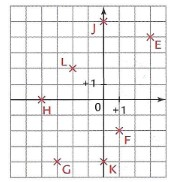
\includegraphics[width=4.5cm]{pictures/pts_dans_le_plan}
\end{center}
}{-}

\addexo{Soit la figure ci-dessous.
\begin{enumerate}
	\item Quel point a pour abscisse $+2$\,?
	\item Quel point a pour ordonnée $-2$\,?
	\item Quelles sont les coordonnes des points $G,A,B$ et $F$\,?
	\item Nommer deux points qui ont la même abscisse.
	\item Nommer deux points qui ont la même ordonnée.
\end{enumerate}
\begin{center}
	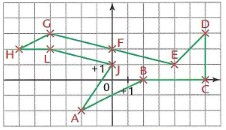
\includegraphics[width=6cm]{pictures/pts_dans_le_plan2}
\end{center}
}{-}

\addexo{Placer les points suivants dans un repère.
$$ A(+5; +4);\, B(+5;+8); C(-3;+4); D(-3;+8). $$
Quelle est la nature du quadrilatère $ABDC$\,?
Et de $ABCD$\,?
}{-}

\addexo{Sur une droite graduée, quelle est la distance des nombres $2; 5; -4; -57$ et l'origine $0$\,?
}{-}

\addexo{Indiquer la valeur absolue des nombres suivants\,:
2; 5; $-4$; $-57$.
}{On note\,: $|2|=2$, $|5|=5$, $|-4|=4$, $|-57|=57$.
}

\defn{La \textbf{valeur absolue} d'un nombre est sa valeur numérique sans tenir compte de son signe.
}


\section{Somme de nombres relatifs}

\addexo{Dans un jeu vidéo, on joue toujours deux parties.
On peut gagner ou perdre des points, marqués par des nombres positifs ou négatifs.
Le tableau ci-dessous regroupe les résultats de quelques jeux de Pierre.
\begin{center}
\begin{tabular}{c|c|c}
	Jeu & 1$^{re}$ partie & 2$^e$ partie \\
	\hline
	a) & +3 & +7 \\
	b) & +9 & +3  \\
	c) & $-4$ & $-2$ \\
	d) & $-5$ & $-6$
\end{tabular}
\end{center}
Effectuer le bilan pour chaque jour en notant chaque fois le calcul associé.
}{-}

\ret{Pour ajouter deux nombres de même signe,
\begin{enumerate}
	\item on garde le signe et
	\item on ajoute leurs valeurs absolues.
\end{enumerate}	
}
\rem{Lorsqu'on a deux signes consécutifs, on doit mettre des parenthèses.
}

\addexo{Ci-dessous sont les résultats de Julie pour le même jeu vidéo.
\begin{center}
\begin{tabular}{c|c|c}
	Jeu & 1$^{re}$ partie & 2$^e$ partie \\
	\hline
	a) & +8 & $-5$ \\
	b) & $-3$ & +7  \\
	c) & $-12$ & $+11$ \\
	d) & $+3$ & $-7$
\end{tabular}
\end{center}
Effectuer le bilan pour chaque jour en notant chaque fois le calcul associé.
}{-}

\ret{Pour ajouter deux nombres de signes contraire,
\begin{enumerate}
	\item on note le signe du nombre relatif ayant la plus grande valeur absolue et
	\item on retranche la plus petite valeur absolue de la plus grande.
\end{enumerate}
}

\addexo{Effectuer les calculs suivants.
\begin{enumerate}
	\item $ (-13)+(+10)= $
	\item $ (-7)+(-4)= $
	\item $ (+9)+(-12)= $
	\item $ (-12)+(+13)= $
	\item $ (+18)+(-24)= $
	\item $ (-46)+(+46)= $
\end{enumerate}
}{-}
\defn{Deux nombres relatifs dont la somme est 0 sont appelés \emph{nombres opposés}.
}

\addexo{Effectuer les calculs suivants.
\begin{enumerate}
	\item $ (-8)+(+12)= $
	\item $ (+9)+(-13)= $
	\item $ (+5)+(-4)= $
	\item $ (-16)+(-18)= $
	\item $ (-17)+(+6)= $
	\item $ (-12)+(+3)= $
\end{enumerate}
}{-}

\addexo{Effectuer les calculs suivants.
\begin{enumerate}
	\item $ (+15)+(-17)= $
	\item $ (-98)+(-3)= $
	\item $ (-75)+(+19)= $
	\item $ (+81)+(-8)= $
	\item $ (+17)+(-21)= $
	\item $ (-23)+(-24)= $
\end{enumerate}
}{-}

\addexo{Effectuer les calculs suivants.
\begin{enumerate}
	\item $ (+65)+(-17)= $
	\item $ (-28)+(-13)= $
	\item $ (+9)+(-36)= $
	\item $ (+18)+(-19)= $
	\item $ (+75)+(-26)= $
	\item $ (-48)+(-42)= $
\end{enumerate}
}{-}

\addexo{Effectuer les calculs suivants.
\begin{enumerate}
	\item $ (-2,45)+(+3,84)= $
	\item $ (+7,8)+(-5,2)= $
	\item $ (+8,1)+(-9,3)= $
	\item $ (-24,8)+(-2,7)= $
	\item $ (-54,2)+(+45,9)= $
	\item $ (+97,5)+(-54,7)= $
\end{enumerate}
}{-}

\addexo{Effectuer les calculs suivants.
\begin{enumerate}
	\item $ (+1,01)+(-1,1)= $
	\item $ (-15,8)+(+23,7)= $
	\item $ (-1)+(+0,1)= $
	\item $ (-58,8)+(-12,2)= $
	\item $ (-99,9)+(+0,01)= $
	\item $ (+12,05)+(-13,07)= $
\end{enumerate}
}{-}

\addexo{Compléter.
\begin{enumerate}
	\item $ (+9,2)+\ldots = -5 $
	\item $ \ldots+(-0,5) = -0,4 $
	\item $ \ldots +(+1,9) = 0 $
	\item $ (-2,01)+\ldots = 0 $
	\item $ (-0)+\ldots = -52,7 $
	\item $ \ldots +(+7,15) = +6,12 $
\end{enumerate}
}{-}

\addexo{Effectuer les calculs suivants.
\begin{enumerate}
	\item $ (-15)+(-9)+(+8)+(-12)+(-8)= $
	\item $ (+91)+(-57)+(+15)+(-26)= $
	\item $ (-13)+(+24)+(+45)+(-49)+(-24)= $
	\item $ (+47)+(-45)+(-87)+(+62)+(+78)= $
	\item $ (-29)+(-74)+(+42)+(-101)+|-17|= $
	\item $ (-76)+(-12)+(+98)+(-45)+|+21|+(+112)= $
\end{enumerate}
}{-}

\ret{Pour effectuer une somme, on peut déplacer les termes dans l'ordre que l'on veut.
C'est la commutativité de l'addition.
}

%\arrow Ex. 22*, 23, 24*, 30, 31*, 32* p.80 ($\Delta$5e)

\addexo{Effectuer les calculs suivants.
\begin{enumerate}
	\item $ (-18)+(-12)+(-11)+(+18)+(+13)= $
	\item $ (-52)+(+48)+(-60)+(+4)= $
	\item $ (+78)+(-60)+(+1)+(-18)= $
	\item $ (+121)+(-88)+(-71)+(+25)+(+8)= $
	\item $ (-19)+(+80)+(-51)+(-55)= $
	\item $ (-324)+(+547)+|-124|+(-327)= $
\end{enumerate}
}{-}

\addexo{Effectuer les calculs suivants.
\begin{enumerate}
	\item $ (+2,8)+(-7,9)+(-2,3)+(+19,2)= $
	\item $ (+1,1)+(-2,2)+(+3,3)+(-4,4)= $
	\item $ (-12,07)+(+19,8)+(-25,4)+(-9,7)+(-1,87) =$
	\item $ (-1,08)+(-2,71)+(+3,87)= $
	\item $ (+15,09)+(+14,3)+(+27,8)+(-0,1)+(-0,09)= $
	\item $ (-27,8)+(-17,05)+(+24,8)+(+16)+(+0,06)+(-0,01)= $
\end{enumerate}
}{-}

\addexo{Calculer mentalement.
\begin{enumerate}
	\item $ (-183)+(+7)+(+12)+(-4)+(+183)= $
	\item $ (-54)+(+87)+(+3)+(+54)+(-87)= $
	\item $ (+68)+(-38)+(-2)+(-68)+(+38)= $
	\item $ (-19)+(-12)+(+19)+(+53)+(+12)= $
	\item $ (+21)+(+47)+(-15)+(-47)+(+9)= $
	\item $ (-64)+(+12)+(-23)+(-8)+(+23)= $
\end{enumerate}
}{-}


%\arrow Ex. 7, 8, 9, 10*, 11*,  p.79 ($\Delta$5e) \datei{Bicher/T5/T5_p.079.jpg} \\
%\arrow Ex. 26 p.80 (Déf. nombres opposés) \datei{Bicher/T5/T5_p.080.jpg}

\addexo{Compléter tel que l'égalité soit vraie.
\begin{enumerate}
	\item $(-4)+(\ldots)=0$
	\item $(\ldots)+(+8)=0$
	\item $(\ldots)+(-7)=0$
	\item $(+5)+(\ldots)=0$
\end{enumerate}
}{-}

\defn{Deux nombres relatifs sont \textbf{opposés} si leur somme est égale à zéro.
}
Exemples\,:
$3$ et $-3$ sont opposés, ainsi que $1,5$ et $-1,5$. De même\,: $-\frac{1}{3}$ est l'opposé de $\frac{1}{3}$.

%\arrow Ex. 27, 28, (29) p.80 ($\Delta$5e)

\addexo{Trouver la valeur de la lettre dans chaque cas.
\begin{enumerate}
	\item $m+(+8)=0$
	\item $(-4)+p=0$
	\item $r+(-6)=0$
	\item $(+7)+t=0$
\end{enumerate}
}{-}




\section{Différence de nombres relatifs}
\addexo{Dans un jeu, Tim a obtenu des cartes avec les points suivants\,:
$$ +7; \quad -2; \quad +5; \quad -6.  $$
\begin{enumerate}
	\item Déterminer la somme de ses points.
\end{enumerate}
Un autre joueur tire une des cartes de Tim.
\begin{enumerate}[start=2]
	\item Déterminer à l'aide du résultat précédent la nouvelle somme lorsque l'autre joueur a tiré la carte avec $+7$.
	\item Même question si l'autre joueur a tiré la carte avec $-6$.
	\item Même question si l'autre joueur a tiré la carte avec $-2$.
	\item Est-il possible de noter les calculs ci-dessus sous forme d'une addition\,?
\end{enumerate}
}{-}

\noindent
Au lieu de retirer la carte avec $-6$, on peut ajouter +6. \\
Au lieu de retirer $+7$, on peut ajouter $-7$ (nombre opposé).

\noindent
\textbf{Conclusion\,:} Retirer un nombre relatif revient à ajouter l'opposé de ce nombre\,:
$$ -(+a) = +(-a) $$
$$ -(-a) = +(+a) $$


\addexo{Calculer.
\begin{enumerate}
	\item $ (+7)-(-5)-(+4)+(-2)= $
	\item $ (-1)+(-1)-(-2)-(+2)= $
	\item $ (-12)-(-59)+(-45)-(-18)= $
	\item $ (-52)+|-21|-(-17)-(-52)= $
	\item $ (+24)+(-56)-(-47)+(-42)-(+32)-(-99)= $
	\item $ (-427)+(-781)-(-547)-(+155)= $
\end{enumerate}
}{-}

\ret{Pour tout nombre $a$\,:
$$\begin{array}{rcl}
	+(+a) &=& +a  \\
	+(-a) &=& -a  \\
	-(+a) &=& -a  \\
	-(-a) &=& +a 
\end{array}$$
}

%\arrow Ex. 34, 35*, 36*, 37, 38*, 39*,  p.81 \datei{Bicher/T5/T5_p.081.jpg}\\
%\arrow Ex. 43, 44*, 45*, 47 p.81 \\
%\arrow Ex. 48 - 53* p.82 \datei{Bicher/T5/T5_p.082.jpg}

\addexo{Calculer.
\begin{enumerate}
	\item $ (-9)-(-4)= $
	\item $ (-8)-(+3)= $
	\item $ (+7)-(+2)= $
	\item $ (+ 16)-(-3)= $
	\item $ (-5)-(-9)= $
	\item $ (+8)-(+15)= $
\end{enumerate}
}{-}

\addexo{Calculer.
\begin{enumerate}
	\item $ (+4)-(-9)= $
	\item $ (+6)-(-3)= $
	\item $ (-6)-(+8)= $
	\item $ (-9)-(-4)= $
	\item $ (+7)-(+3)= $
	\item $ (+5)-(+9)= $
\end{enumerate}
}{-}

\addexo{Calculer.
\begin{enumerate}
	\item $ (+14)-(-17)= $
	\item $ (+ 26)- (- 18)= $
	\item $ (- 46)-(+38)= $
	\item $ (+17)- (+ 23)= $
	\item $ (-39)-(-14)= $
	\item $ (+35)-(+49)= $
\end{enumerate}
}{-}

\addexo{Trouver la valeur de la lettre dans chaque cas.
\begin{enumerate}
	\item $e-(- 8) = 0$
	\item $f-(+5) = 0$
	\item $(-9)-g = 0$
	\item $h-(+7) = 0$
\end{enumerate}
}{-}

\addexo{Calculer.
\begin{enumerate}
	\item $(- 4,8) + (+ 3,5)=$
	\item $ -2,9)-(-3,2)=$
	\item $(+ 8,2) - (+ 5,6)=$
	\item $(+ 5,8) + (- 2,4)=$
\end{enumerate}
}{-}

\addexo{Calculer.
\begin{enumerate}
	\item $(+ 2,5) + (- 4,5)=$
	\item $(-5,5)-(-3,5)=$
	\item $(+7,5)-(+4,5)=$
	\item $(+6,5)-(+9,5=$
	\item $(- 8,5) + (+ 9,5)=$
	\item $(- 6,5) - (- 8,5)=$
\end{enumerate}
}{-}

\addexo{Calculer.
\begin{enumerate}
	\item $(+ 6,2) - (+ 8,2)=$
	\item $(+ 4,5) - (+ 3,5)=$
	\item $(+8,6)+ (-4,3)=$
	\item $(+9,3) - (- 3,8)=$
	\item $(- 1,8) - (- 1,3)=$
	\item $(- 5,4) + (+ 7,2)=$
\end{enumerate}
}{-}

\addexo{Calculer.
\begin{enumerate}
	\item $(+7)-(-10)=$
	\item $(+6) + (-3)=$
	\item $(-4)-(+12)=$
	\item $(-9)-(-4)=$
	\item $(-17) + (-13)=$
	\item $(+5)-(+9)=$
\end{enumerate}
}{-}


\section{Écriture simplifiée}
Pour effectuer une suite de calculs, on additionne les nombres deux à deux. \\
(Faire un exercice pour montrer le regroupement des nombres deux à deux.) \\

\addexo{Écrire d'abord en écriture simplifiée, puis calculer.
\begin{enumerate}
	\item $ (+1)-(+2)+(-3)-(-4)= $
	\item $ (-1,24)+(-2,59)-(-1,4)= $
	\item $ (+6,75)-(+4,07)+(+4,8)= $
	\item $ (-1,01)+(+2,24)-(+1,98)-(-0,09)= $
	\item $ (+10,2)-(+4,72)-|-1|= $
	\item $ (+9,74)-(-10,21)+(-0,85)-(-0,99)= $
\end{enumerate}
}{-}

\addexo{Calculer.
\begin{enumerate}
	\item $ -12+18-9-12= $
	\item $ 45-13-78+24= $
	\item $ -1,28+5,78-1,22= $
	\item $ -(-0,05+7,54)-2,54-1,7= $
	\item $ -45-(45-8+5)-9 =$
	\item $ 29+(68-73)-32= $
\end{enumerate}
}{-}

\addexo{Calculer mentalement.
\begin{enumerate}
	\item $ 54-108+54= $
	\item $ 30-32+40-50+20= $
	\item $ 72-68+53-72+15= $
	\item $ 98-24-24= $
	\item $ -121+30+22-31= $
	\item $ 35-85+75-15= $
\end{enumerate}
}{-}

\arrow Ex. 101, 102, 105, 106, 107, 109 p.57f (CP)
\\
\arrow Ex. 54 p.82
\\
\arrow Ex. 55', 56*, 57* p.82

Beispiller maan fir di nei convention anzeféiren

\ret[Convention d'écriture]{
Dans une suite d'additions de nombres relatifs, on supprime les \uline{signes d'addition} et les parenthèses autour de chaque nombre. En plus, on peut supprimer le signe d'un nombre positif en début de calcul.
}
\arrow Ex. 58, 59, 60*-62* p.82 \\
%\arrow Ex. 63-65*, 67-70* p.83 \datei{Bicher/T5/T5_p.083.jpg}

Selon disposition du temps\,: problèmes et énigmes.



\section{Multiplication et division de nombres relatifs}
\subsection{Rappels}
\addexo{Joe possède 12 cartes à collectionner.
Il achète 6 paquets, chacun contenant 8 nouvelles cartes. Combien de cartes possède-t-il\,?
}{$12 +\underbrace{6 \cdot 8}_{=48} = 12 + 48 = 60 $  (\og Punkt vor Strich!\fg) \\
Après l'achat, Joe compte 60 cartes.
}

\addexo{Effectuer les calculs suivants.
Indiquer au moins deux facteurs et deux termes.
\begin{multicols}{5}
\noindent
$  11 +10\,:5= \\
  9 \cdot 5 - 8 \cdot 8= \\
  6 \cdot (7 -2)= \\
  4 \cdot 5 -6= \\
  (4 +2\cdot 8) \cdot 5=$
\end{multicols}
}{-}

\ret{Afin d'effectuer une suite de calculs on doit respecter l'ordre suivant\,:
\begin{enumerate}
  \item D'abord, on effectue les calculs entre parenthèses,
  \item ensuite les multiplications et divisions.
  \item Puis les sommes (et les différences).
\end{enumerate}
}

%\arrow Ex. 14 p.17 (T4) \datei{Bicher/T4/T4_p.017.jpg}



\subsection{Règles de calcul}
\stitle{Activité}
$$\begin{array}[t]{ll}
	(+2) \cdot (+3)  =& +6 \\
	(+1) \cdot (+3)  =& +3 \\
	(+0) \cdot (+3)  =&  0 \\
	(-1) \cdot (+3)  =& -3 \\
	(-2) \cdot (+3)  =& -6
\end{array}$$

\ret{Un nombre négatif multiplié par un nombre positif donne un nombre négatif.
}

$$\begin{array}{ll}
	(-2) \cdot (+3)  =& -6 \\
	(-2) \cdot (+2)  =& -4 \\	
	(-2) \cdot (+1)  =& -2 \\
	(-2) \cdot (+0)  =& 0  \\
	(-2) \cdot (-1)  =& +2 \\
	(-2) \cdot (-2)  =& +4	
\end{array}$$

\ret{Pour multiplier/diviser deux nombres relatifs,
on détermine d'\textbf{abord le signe} du produit\,:
$$ \boxed{%
\begin{array}{rrrr}
 (+..) & \cdot & (+..) &=+.. \\
 (+..) & \cdot & (-..) &=-.. \\
 (-..) & \cdot & (+..) &=-.. \\
 (-..) & \cdot & (-..) &=+..
\end{array}
} $$
Ensuite, on multiplie les \textbf{nombres} sans signe.
}

\addexo{Calculer.
\begin{enumerate}
	\item $ (-6)\cdot(+5)= $
	\item $ (-8)\cdot(-7)= $
	\item $ (-12)\cdot(-11)= $
	\item $ (-15)\cdot(+15)= $
	\item $ (+32)\cdot(-25)= $
	\item $ (-50)\cdot(-42)= $
\end{enumerate}
}{-}


\addexo{Calculer.
\begin{enumerate}
	\item $ (-2,5)\cdot(-1,5)= $
	\item $ (+6,7)\cdot(-12)= $
	\item $ (-18)\cdot(+20)= $
	\item $ -9,1\cdot(+11)= $
	\item $ 19\cdot(-3)= $
	\item $ -6\cdot 21= $
\end{enumerate}
}{-}

\rem{Lorsqu'on a deux signes d'opération ($+;-;\cdot;\,:$) consécutifs, alors on doit mettre des parenthèses.
}


À l'aide de la multiplication $(+3)\cdot(-4)=-12$, on obtient deux divisions\,: \\
\begin{center}
	$ (-12)\,:(+3)=-4 $ et $ (-12)\,:(-4)=+3 $.
\end{center}
\ret{Les règles de calcul pour la division correspondent à ceux de la multiplication\,:
\begin{enumerate}
	\item D'abord on note le signe,
	\item ensuite on divise les nombres sans signe.
\end{enumerate}
}


\ret{Pour multiplier/diviser deux nombres relatifs,
on détermine d'abord le signe du produit\,:
\begin{itemize}
	\item si les deux nombres sont du même signe, le produit est positif.
	\item si les deux nombres sont de signes contraires, le produit est négatif.
\end{itemize}
Ensuite, on multiplie les deux nombres sans signe.
}

%\arrow Ex. 30-41 p.18 \datei{Bicher/T4/T4_p.018.jpg}

A l'aide de la multiplication $(+3)\cdot(-4)=-12$, on obtient deux divisions\,: \\
\begin{center}
	$ (-12)\,:(+3)=-4 $ et $ (-12)\,:(-4)=+3 $.
\end{center}
De plus\,:
$$ (-2)\cdot(-5)=+10 \Rightarrow (+10)\,:(-2)=-5 $$
Par conséquent\,:
$$ \boxed{%
\begin{array}{rrr}
 (+..) & \cdot (+..) &=+.. \\
 (+..) & \cdot (-..) &=-.. \\
 (-..) & \cdot (+..) &=-.. \\
 (-..) & \cdot (-..) &=+..
\end{array}
} $$
\rem{\begin{enumerate}[label=$\bullet$]
	\item $(-12)\,:(+3) = \dfrac{-12}{+3} =-\dfrac{12}{3} $
	\item $(+10)\,:(-2) = \dfrac{+10}{-2} =-\dfrac{10}{2} $
	\item $(-12)\,:(-4) = \dfrac{-12}{-4} =+\dfrac{12}{4} $
\end{enumerate}
}

%\arrow Ex. 46, 47 p.18 \\
%\arrow Ex. 48-57 p.19 \datei{Bicher/T4/T4_p.019.jpg} \\
%\arrow Ex. 98, 100 p.21 \datei{Bicher/T4/T4_p.021.jpg} \\
%\arrow Ex. 105 p.23 \datei{Bicher/T4/T4_p.023.jpg} \\

\ret
 {Quand on multiplie plusieurs nombres relatifs, alors le signe du produit est
  \begin{itemize}
    \item positif, si le nombre de facteurs négatifs est pair.
    \item négatif, si le nombre de facteurs négatifs est impair.
  \end{itemize}
 }
\arrow Ex.45 p.18 \\
\arrow Ex.87 p.21 (problème)

\stitle{Exemple}
Comparer les calculs suivants\,:
$$\begin{array}[t]{rl}
 (-25) \cdot (-17) \cdot (+4) \\
  = (+425) \cdot (+4) \\
  = 1\,700
\end{array}
\hspace{1cm}
\begin{array}[t]{rl}
  \underbrace{(-25)\cdot(+4)}_{= -100} \cdot (-17) \\
  = 1\,700
 \end{array}$$

Pour faciliter le calcul on peut regrouper les facteurs\,:

\prop[Commutativité de la multiplication]
{Multiplier plusieurs nombres relatifs peut se faire dans n'importe quel ordre.
}

\stitle{Le carré d'un nombre}
Comparer les calculs suivants\,:
\[\begin{array}{rlp{1cm}rl}
 & (-4)^2 &&& -4^2 \\
 = &(-4) \cdot (-4) &&= &-4 \cdot 4 \\
 = &16 &&= &-16
\end{array}\]
Dans le premier exemple, le carré se rapporte à tout ce qui est écrit entre parenthèses; il faut multiplier $-4$ par $-4$.
Dans le deuxième exemple, le carré se rapporte seulement au nombre $4$ et non pas au signe parce que $4$ est le seul nombre qui se trouve en-dessous de l'exposant $2$. Le signe est copié (une fois) et le nombre $4$ est multiplié par $4$.

\defn{Dans une expression du type $a^n$, $a$ est appelé la \uline{base} et $n$ l'\uline{exposant}.
 }


%\arrow Ex. 42-44* p.18 \datei{Bicher/T4/T4_p.018.jpg} \\

Effectuer les calculs suivants\,:
\[ 3+(-7)^2= \qquad (3-7)^2\,:8+5= \]
\ret{On effectue d'abord les calculs entre parenthèses, puis les carrés et ensuite les multiplications/divisions avant les sommes/soustractions.
}





\addexo{Déterminer\,:
\begin{enumerate}
	\item le produit de 99 facteurs tous égaux à $-1$,
	\item la somme de 99 termes tous égaux à $-1$,
	\item la somme de tous les termes de 1 à 99,
	\item le signe du produit de tous les facteurs allant de $-67$ à $-154$.
\end{enumerate}
}{-}
 
\addexo{Calculer.
\begin{enumerate}
	\item $ (-1)^3= $
	\item $ (-5)^0= $
	\item $ -5^0= $
	\item $ (4,08-7,1+2,12)^2= $
	\item $ -5\cdot(-17+25-42)= $
	\item $ -12 -\left[ 5-3 \cdot (-54) +1 \right]= $
\end{enumerate}
}{-}

\addexo{Calculer.
\begin{enumerate}
	\item $ -12\,:3= $
	\item $ -45\,: (-15)= $
	\item $ 60\,: (-30)= $
	\item $ -(-35)\,:(-5)= $
	\item $ 80\,:(-100)= $
	\item $ (-8)\,:(-0,1)= $
\end{enumerate}
}{-}

\addexo{Calculer.
\begin{enumerate}
	\item $ -45\,:1\,000= $
	\item $ -45,7\,:(-100)= $
	\item $ 45,7-100= $
	\item $ (-15)\,:(-6)= $
	\item $ 5 \cdot (-125)= $
	\item $ 1\,:(-1)= $
\end{enumerate}
}{-}

\addexo{Soit $A= b^2-4ac$.
Déterminer $A$ pour\,:
\begin{enumerate}
	\item $a=-1;\quad b=2; \quad c=-5$.
	\item $a=5;\quad b=-5; \quad c=-6$.
	\item $a=-7;\quad b=-1; \quad c=-1$.
\end{enumerate}
}{-}

\addexo{Vrai ou faux. Justifier chaque fois.
\begin{enumerate}
	\item $-x$ est un nombre négatif.
	\item $x^2$ est un nombre positif.
	\item Multiplier un nombre $x$ par $-2$ donne un nombre inférieur à $x$.
	\item Diviser un nombre $x$ par $-0,1$ donne un nombre inférieur à $x$.
\end{enumerate}
}{-}

\addexo{Calculer.
\begin{enumerate}
	\item $ 160-(3\cdot5^2-3\cdot5)= $
	\item $ 142-(50-3 \cdot 6^2)= $
	\item $ 2 \cdot 10^2 -4 \cdot (5-5^2)+20= $
	\item $ -4^2 \cdot \left( 1+8+(-4)^2\right)= $
	\item $ (18-4\cdot 5) \cdot (6 \cdot 3-10) \cdot(-3^2)= $
	\item $ \left( 7-4^2 \right) \cdot (-18:3+12 ) \cdot  \left(2\cdot 3^2 -20 \right)= $
\end{enumerate}
}{-}

Ex. 115/116/119 p.60 (CP)

%\arrow Ex. 65, 66* p.19 \datei{Bicher/T4/T4_p.019.jpg} \\
%\arrow Ex. 101, 104 p.23 \datei{Bicher/T4/T4_p.023.jpg} \\
%\arrow Ex. 91,92 p.21 \datei{Bicher/T4/T4_p.021.jpg}

















%%% -------------------------------- EXERCICEN PRINTEN

\clearpage
\begin{exercices}
\foreach \x/\y in \exos
{\exo \x
 \ifnum\value{exo}=7 \columnbreak \fi
 \ifnum\value{exo}=17 \columnbreak \fi
 \ifnum\value{exo}=21 \columnbreak \fi
 \ifnum\value{exo}=25 \columnbreak \fi
 \ifnum\value{exo}=29 \columnbreak \fi
 \ifnum\value{exo}=33 \columnbreak \fi
 \ifnum\value{exo}=38 \columnbreak \fi
 }
\end{exercices}



%\clearpage
%\begin{solutions}
%\foreach \x/\y in \exos
% {\sol \y
%  }
%\end{solutions} % 7-8 semaines

%\newcommand{\addexoInline}[2]
%{\addexo{#1}{#2}%
%}
%\newcommand{\retenir}[2][]
%{\ret[#1]{#2}%
%}
%\newcommand{\midblank}[1]
%{\ldots%
%}
%\renewcommand{\Box}
%{{\ldots}%
%}

\chapter{Puissances}
\section{Puissances à exposants positifs}

\addexoInline{Le roi Belkib (Indes) promit une récompense fabuleuse à qui lui proposerait une distraction qui le satisferait. Lorsque le sage Sissa, fils du Brahmine Dahir, lui présenta le jeu d'échecs, le souverain, demanda à Sissa ce que celui-ci souhaitait en échange de ce cadeau extraordinaire. \\
Sissa demanda au prince de déposer un grain de riz sur la première case, deux sur la deuxième, quatre sur la troisième, et ainsi de suite pour remplir l'échiquier en doublant la quantité de grain à chaque case. \\
Le prince accorda immédiatement cette récompense sans se douter de ce qui allait suivre:
\begin{enumerate}
	\item Déterminer le nombre de grains de riz sur la 11e case.
	\item Déterminer le nombre de grains de riz sur la 21e case.
	\item Estimer le nombre de grains de riz sur la 64e case.
\end{enumerate}
}{ $2^{10}=1\,024$ \\
$2^{20} \approx 1\,mio$ \\
$2^{63}= 9\,223\,372\,036\,854\,775\,808$ grains $\approx$ 500 fois la production \textbf{actuelle} d'une année.
}




\stitle{Exemples}
\begin{enumerate}[label=$\star$]
  \item $\underbrace{2\cdot2\cdot2\cdot2}_\text{{\red 4} facteurs égaux}=2^{\red 4}$ (On lit: "2 exposant 4")
  \item $\underbrace{5\cdot5\cdot5\cdot5\cdot5\cdot5}_\text{{\red 6} facteurs égaux}=5^{\red 6}$ (5 exposant 6)
  \item $\underbrace{3\cdot3}_\text{{\red 2} facteurs égaux}=3^{\red 2}$ (3 exposant 2 ou 3 au carré)
  \item $\underbrace{4\cdot4\cdot4}_\text{{\red 3} facteurs égaux}=4^{\red 3}$ (4 exposant 3 ou 4 au cube)
\end{enumerate}

\defn{Soit $x$ un nombre quelconque et $n$ un nombre entier (strictement) positif. Alors
$$ x^{\red n}=\underbrace{x\cdot x\cdot x\cdot.....\cdot x}_\text{{\red n} facteurs égaux} $$
est une \textbf{puissance} et
\begin{enumerate}[label=$\star$]
  \item $x$ s'appelle \textbf{base}
  \item $n$ s'appelle \textbf{exposant}
\end{enumerate}
On pose:
$$ x^1=x; \qquad x^0=1. $$
Mais $0^0$ n'existe pas!
}

\addexoInline{Calculer.
\begin{multicols}{2}\vspace{-\baselineskip}
\begin{enumerate}
  \item $ 5^3= $
  \item $ 0,3^2= $
  \item $ 0,1^3= $
  \item $ 2^4= $
  \item $ (-4)^3= $
  \item $ (-1,3)^2= $
\end{enumerate}
\end{multicols}
}{-}

%\retenir[Puissances usuelles]{
%	\begin{multicols}{3}
%		\begin{itemize}
%			\item $ 1^2 = \midblank{2} $
%			\item $ 2^2 = \midblank{2} $
%			\item $ 3^2 = \midblank{2} $
%			\item $ 4^2 = \midblank{2} $
%			\item $ 5^2 = \midblank{2} $
%			\item $ 6^2 = \midblank{2} $
%			\item $ 7^2 = \midblank{2} $
%			\item $ 8^2 = \midblank{2} $
%			\item $ 9^2 = \midblank{2} $
%			\item $ 10^2 = \midblank{2} $
%			\item $ 11^2 = \midblank{2} $
%			\item $ 12^2 = \midblank{2} $
%			\item $ 13^2 = \midblank{2} $
%			\item $ 14^2 = \midblank{2} $
%			\item $ 15^2 = \midblank{2} $
%		\end{itemize}
%	\end{multicols}\vspace{0.5cm}
%	\begin{multicols}{3}
%		\begin{itemize}
%			\item $ 1^3 = \midblank{2} $
%			\item $ 2^3 = \midblank{2} $
%			\item $ 3^3 = \midblank{2} $
%			\item $ 4^3 = \midblank{2} $
%			\item $ 5^3 = \midblank{2} $
%		\end{itemize}
%	\end{multicols}\vspace{0.5cm}
%	\begin{multicols}{3}
%		\begin{itemize}
%			\item $ 2^0 = \midblank{2} $
%			\item $ 2^1 = \midblank{2} $
%			\item $ 2^2 = \midblank{2} $
%			\item $ 2^3 = \midblank{2} $
%			\item $ 2^4 = \midblank{2} $
%			\item $ 2^5 = \midblank{2} $
%			\item $ 2^6 = \midblank{2} $
%			\item $ 2^7 = \midblank{2} $
%			\item $ 2^8 = \midblank{2} $
%			\item $ 2^9 = \midblank{2} $
%			\item $ 2^{10} = \midblank{2} $
%		\end{itemize}
%	\end{multicols}
%}

\addexo{calculer les carrés des entiers positifs jusqu'à 15.
}{-}

\addexo{Calculer les cubes des entiers positifs jusqu'à 5.
}{-}

\addexo{Calculer les puissances de base 2 et d'exposants entiers jusqu'à 10.
}{-}

\addexoInline{Calculer.
\begin{multicols}{2}\vspace{-\baselineskip}
\begin{enumerate}
  \item $ \left(\dfrac{1}{3}\right)^4= $
  \item $ 13^0= $
  \item $ \left(-\dfrac{1}{2}\right)^5= $
  \item $ \left(-\dfrac{1}{8}\right)^1= $
  \item $ (-7)^0= $ 
  \item $ -7^0= $
\end{enumerate}
\end{multicols}
}{-}

\addexoInline{Vrai ou faux. Justifier.
\begin{enumerate}
  \item $2^4$ est le double de $2^3$.
  \item $2^3=3^2$.
  \item $2^4=2 \cdot 4$
  \item $5^2$ est la moitié de $5^4$.
\end{enumerate}
}{-}

\addexoInline{Trouver pour chaque cas $n$.
	\begin{multicols}{2}\vspace{-\baselineskip}
\begin{enumerate}
  \item $27 = 3^n$
  \item $ n^3=125 $
  \item $ 5^n=125 $
  \item $ n^2=81 $
  \item $ 5^n = 1 $
  \item $ n^10 = 0 $
\end{enumerate}
\end{multicols}
}{-}

\addexoInline{Calculer.
	\begin{multicols}{2}\vspace{-\baselineskip}
\begin{enumerate}
  \item $ 0,2^3= $
  \item $ 0,04^2= $
  \item $ 1,3^2= $
  \item $ 10^2 \cdot 10^3 \cdot 10^5 = $
  \item $ 2^3 \cdot 3^2 = $
  \item $ 2^3 \cdot 2^3 = $
\end{enumerate}
\end{multicols}
}{-}

\addexoInline{Écrire sous la forme d'une puissance $a^n$.
	\begin{multicols}{2}\vspace{-\baselineskip}
\begin{enumerate}
  \item $ 6^2 \cdot 6^3 = $
  \item $ 5 \cdot 5^3= $
  \item $ 7^2 \cdot 7^4= $
  \item $ 1^3 \cdot 1^8= $
  \item $ 11^{12} \cdot 11^{13}= $
  \item $ 2^3 \cdot 3^2 = $
\end{enumerate}
\end{multicols}
}{-}

\addexoInline{Déterminer si le résultat est positif ou négatif.
	\begin{multicols}{2}\vspace{-\baselineskip}
\begin{enumerate}
  \item $ (-2)^2= $
  \item $ -2^2= $
  \item $ -(-2)^2= $
  \item $ -(-81)^3= $
  \item $ -3^{20}= $
  \item $ -1^2 \cdot (-5)^{3}= $
\end{enumerate}
\end{multicols}
}{-}

\addexoInline{Calculer.
	\begin{multicols}{2}\vspace{-\baselineskip}
\begin{enumerate}
  \item $ \left(\dfrac{2}{5}\right)^2= $
  \item $ \dfrac{2^2}{5}= $
  \item $ \left(\dfrac{-5}{3}\right)^2= $
  \item $ \dfrac{-5^2}{3}= $
\end{enumerate}
\end{multicols}
}{-}



\section{Puissances à exposants négatifs}
Considérons le tableau suivant\,:
$$\begin{array}{rrcll}
  \text{exp.} & \text{puiss.} && \text{rés.} \\
\hline
 -1 \downarrow & 3^3 &=& 27 & \downarrow :3 \\
 -1 \downarrow & 3^2 &=& 9 & \downarrow :3 \\
 -1 \downarrow & 3^1 &=& 3 & \downarrow :3 \\
 -1 \downarrow & 3^0 &=& 1 & \downarrow :3 \\
 -1 \downarrow & 3^{-1} &=& \frac{1}{3} & \downarrow :3 \\
 -1 \downarrow & 3^{-2} &=& \frac{1}{9} & \downarrow :3 \\
 & 3^{-3} &=& \frac{1}{27}
\end{array}$$

%%%% Fir base just mat der base 10
$$\begin{array}{rrcll}
  \text{exp.} & \text{puiss.} && \text{rés.} \\
\hline
 -1 \downarrow & 10^3 &=& 1\,000 & \downarrow :10 \\
 -1 \downarrow & 10^2 &=& 100 & \downarrow :10 \\
 -1 \downarrow & 10^1 &=& 10 & \downarrow :10 \\
 -1 \downarrow & 10^0 &=& 1 & \downarrow :10 \\
 -1 \downarrow & 10^{-1} &=& \frac{1}{10} & \downarrow :10 \\
 -1 \downarrow & 10^{-2} &=& \frac{1}{10} & \downarrow :10 \\
 & 10^{-3} &=& \frac{1}{1\,000}
\end{array}$$

\defn{Soit $x$ un nombre quelconque {\red non nul}. Soit $n$ un entier positif. Alors
$$ x^{-n}=\dfrac{1}{x^n} $$
est \textbf{l'inverse de $x^n$}.
}


%\addexoInline{Calculer.
%\begin{multicols}{2}\vspace{-\baselineskip}
%\begin{enumerate}
%  \item $ 2^{-3} $
%  \item $ 3^{-2} $
%  \item $ 0,1^{-2} $
%  \item $ (-5)^{-1} $
%  \item $ (-7)^{-2} $
%  \item $ -7^{-2} $
%\end{enumerate}
%\end{multicols}
%}{-}

\rem{\vspace{-\baselineskip}
\begin{enumerate}[label=$\cdot$]
  \item $\dfrac{1}{x}$ est l'inverse de $x$ si $x \overset{!}{\neq} 0$.
  \item Si l'exposant est $-1$, il suffit d'inverser le nombre entre parenthèses.
\end{enumerate}
}

%\addexoInline{Calculer.
%	\begin{multicols}{2}\vspace{-\baselineskip}
%\begin{enumerate}
%  \item $ 2^{-1} $
%  \item $ 5^{-1} $
%  \item $ 4^{-1} $
%  \item $ 10^{-2= $
%  \item $ 10^{-4} $
%  \item $ 2^{-2} $
%\end{enumerate}
%\end{multicols}
%}{-}

\addexoInline{Écrire sous forme d'une puissance $a^n$.
\begin{multicols}{2}\vspace{-\baselineskip}
\begin{enumerate}
  \item $ \dfrac{1}{10} $
  \item $ \dfrac{10}{1\,000} $
%  \item $ 64 $
  \item $ 0,01  $
%  \item $ \dfrac{1}{100} $
  \item $ 0,000\,1 $
%  \item $ 27 $
  \item $ 100 \cdot 0,1 $
  \item $ \dfrac{0,01}{100} $
\end{enumerate}
\end{multicols}
}{-}

%
%Exemple
%$$\begin{array}[t]{rcl}
%10^2 &=& 100 \\
%10^1 &=& 10 \\
%10^0 &=& 1 \\
%10^{-1} &=& \dfrac{1}{10}=0,1 \\
%10^{-2} &=& 0,01 \\
%10^{-3} &=& 0,001
%\end{array}$$

\prop{Si $n$ est un entier positif, alors:
$$ 10^n=1\underbrace{000.....00}_{\text{n zéro}} $$
$$ 10^{-n}=\underbrace{0,00.....00}_{\text{n zéro}}1 $$
}

\addexoInline{Écrire sous forme d'un nombre décimal.
\begin{multicols}{2}\vspace{-\baselineskip}
\begin{enumerate}
  \item $ 10^{-4} $
  \item $ 10^9 $
  \item $ 10^1 $
  \item $ 10^{-5} $
  \item $ 10^0 $
  \item $ 10^{-3} $
\end{enumerate}
\end{multicols}
}{-}

\addexoInline{Écrire sous forme d'un nombre décimal.
\begin{multicols}{2}\vspace{-\baselineskip}
\begin{enumerate}
	\item $ 4,5 \cdot 10^{2} $
	\item $ 27 \cdot 10^4 $
	\item $ 0,072 \cdot 10^5 $
	\item $ 350 \cdot 10^{-2} $
	\item $ 12 \cdot 10^{-4} $
	\item $ 0,045 \cdot 10^{-2} $
\end{enumerate}
\end{multicols}
}{-}

\addexoInline{Écrire sous forme d'une puissance de base 10.
\begin{multicols}{2}\vspace{-\baselineskip}
\begin{enumerate}
  \item 100
  \item 0,000\,1
  \item un dixième
  \item un milliard
  \item un million
  \item un millionième
\end{enumerate}
\end{multicols}
}{-}

\addexoInline{Calculer.
\begin{multicols}{2}
\begin{enumerate}
  \item $ 25,36 : 0,001 $
  \item $ 25,47 \cdot 0,01 $
  \item $ 0,000\,7 : 0,01 $
  \item $ 123\,456 : 0,000\,01 $
  \item $ 1,2 \cdot 0,1 $
  \item $ 1,2 : 0,1 $
\end{enumerate}
\end{multicols}
}{-}




\section{La notation scientifique}
Cette notation est utilisée pour écrire des nombres très grands ou très petits.
La vitesse de la lumière par exemple est environ\,:
$$ 300\,000\,000\ m/s = 3 \cdot 10^8\ m/s. $$

\defn{La notation scientifique d'un nombre positif est\,:
$$ a \cdot 10^n $$
où $a$ est un nombre tel que $1 \leq a < 10$ \\
et $n$ est un entier (positif ou négatif).
}

\addexoInline{Compléter.
\begin{enumerate}
	\item $ 87\,000 = 8,7 \cdot 10^\Box $
	\item $ 1\,540 = 1,54 \cdot 10^\Box $
	\item $ 670\,000 = 6,7 \cdot 10^\Box $
	\item $ 920\,000 = 9,2 \cdot 10^\Box $
	\item $ 0,038 = 3,8 \cdot 10^\Box $
	\item $ 0,001\,59 = 1,59 \cdot 10^\Box $
\end{enumerate}
}{-}

\addexoInline{Compléter.
\begin{enumerate}
	\item $ 0,000\,035 = 3,5 \cdot 10^\Box $
	\item $ 0,043\,2 = 4,32 \cdot 10^\Box $
	\item $ 0,000\,45 = 4,5 \cdot 10^\Box $
	\item $ 0,78 = 7,8\cdot 10^\Box $
	\item $ 5\,457\,000 = 5,457 \cdot 10^\Box $
	\item $ 0,000\,5 = 5 \cdot 10^\Box $
\end{enumerate}
}{-}

\addexoInline{Parmi les nombres suivants, quels sont ceux qui sont écrits en notation scientifique\,? Expliquer.
\begin{multicols}{2}
\begin{enumerate}
  \item $ 3,8 \cdot 10^5 $
  \item $ 0,54 \cdot 10^{-4} $
  \item $ 5,9 \cdot 4^{10} $
  \item $ 6,92 \cdot 10^{-5} $
  \item $ 34 \cdot 10^5 $
  \item $ 0,6 \cdot 10^5 $
\end{enumerate}
\end{multicols}
}{-}

\addexoInline{Écrire en notation scientifique.
\begin{multicols}{2}
\begin{enumerate}
  \item $ 80\,000\,000\,000\,000 $
  \item $ 4\,500\,000\,000 $
  \item $ 0,000\,000\,000\,000\,001 $
  \item $ -0,000\,003\,9 $
  \item $ -0,5 $
  \item $ 1 $
\end{enumerate}
\end{multicols}
}{-}

\addexoInline{Écrire en notation scientifique.
\begin{multicols}{2}
\begin{enumerate}
	\item $ 45\,000 $
	\item $ 654\,000\,000 $
	\item $ 0,000\,073 $
	\item $ 0,000\,000\,745 $
	\item $ 0,67 $
	\item $ 456,78 $
\end{enumerate}
\end{multicols}
}{-}

\addexoInline{Écrire en notation scientifique.
\begin{multicols}{2}
\begin{enumerate}
	\item $ 23 \cdot 10^4 $
	\item $ 666 \cdot 10^{-3} $
	\item $ 0,067\,8 \cdot 10^4 $
	\item $ 0,056 \cdot 10^5 $
	\item $ 56\,780 \cdot 10^{-6} $
	\item $ 4,76 \cdot 10^{-1} $
\end{enumerate}
\end{multicols}
}{-}

\addexoInline{Écrire en notation scientifique.
\begin{multicols}{2}
\begin{enumerate}
	\item $ 47\,000 \cdot 10^5 $
	\item $ 0,052 \cdot 10^4 $
	\item $ 73\,000\,000 \cdot 10^{-3} $
	\item $ 456,78 \cdot 10^{5} $
\end{enumerate}
\end{multicols}
}{-}

\addexoInline{Écrire en notation scientifique.
\begin{multicols}{2}
\begin{enumerate}
	\item $ 654 \cdot 10^{21} $
	\item $ 769 \cdot 10^{-13} $
	\item $ 0,000\,8 \cdot 10^{18} $
	\item $ 5\,780\,000 \cdot 10^{-8} $
	\item $ 876,678 \cdot 10^{15} $
	\item $ 43,679 \cdot 10^{-24} $
\end{enumerate}
\end{multicols}
}{-}



%%%% exercicen aus dem T5
%\arrow Ex 59-61, 63, 66 p.98


%\stitle{Comparaison de deux nombres positifs écrits en notation scientifique}
%\stitle{Exercice:} Compléter par $>$ ou $<$.
%\begin{enumerate}[label=\alph*), series=exemples]
%  \item $ 6 \cdot 10^7 < 3 \cdot 10^9 $
%  \item $ 5 \cdot 10^4 > 8 \cdot 10^{-5} $
%  \item $ 3,2 \cdot 10^-5 > 3,4 \cdot 10^{-9} $ \\
%\textbf{Conclusion:} Si les exposants des puissances de base 10 sont différents alors le plus grand nombre est celui avec le plus grand exposant.
%  \item $ 3\cdot 10^3 > 2 \cdot 10^3 $
%  \item $ 2\cdot 10^{-2} < 4 \cdot 10^{-2} $
%  \item $ 4,021\cdot 10^5 > 4,201 \cdot 10^5 $ \\
%\textbf{Conclusion:} Si les exposants des puissances de base 10 sont égaux alors le plus grand nombre est celui avec le plus grand facteur a.
%\end{enumerate}


\addexoInline{Donner l'écriture scientifique de la masse de ces planètes, puis les ranger par ordre croissant\,! \\
\begin{tabular}{lr}
	Mars & $ 64 185\cdot10^{19} $ \\
	Jupiter & $ 0,189\cdot10^{28}	$ \\
	Uranus & $ 886,31\cdot10^{23}	$ \\
	Vénus & $ 0,048 7\cdot10^{26}$
\end{tabular}
}{-}
\addexoInline{Donner l'écriture scientifique de la masse de ces atomes, puis les ranger par ordre croissant\,! \\
\begin{tabular}{lr}
	Uranium & $ 0,395\cdot10^{-24}$ \\
	Aluminium & $4,48\cdot10^{-26}$ \\
	Or & $32,7\cdot10^{-26}	$ \\
	Fer & $9274\cdot10^{-29}$ \\
	Cuivre & $1055\cdot10^{-28}$
\end{tabular}
}{-}




\prop[Règles de calcul avec puissances]{
Pour $a, b$ des nombres réels et $n, p$ des nombres entiers.
\begin{enumerate}[label=$\bullet$]
  \item $ a^n \cdot a^p = a^{n+p}$
  \item $ \left(a^n\right)^p = a^{n\cdot p}$ \id{net am cours de base (6G)}
  \item $ a^{n}\cdot b^n  = \left(a\cdot b\right)^n $\id{net am cours de base (6G)}
  \item $ \dfrac{a^n}{a^p} = a^{n-p} \qquad (a \neq 0)$
%  \item $ \left(\dfrac{a}{b}\right)^n = \dfrac{a^n}{b^n}$
%  \item $ \left(\dfrac{a}{b}\right)^{-n} = \left(\dfrac{b}{a}\right)^n$
\end{enumerate}
}
\rem{Il faut avoir un produit/quotient pour appliquer les règles de calcul avec puissances\,: \\
{\red C1\,: multiplication} \\
Ensuite, on recopie\,:
\begin{enumerate}
	\item une fois la base si elles sont égales et on ajoute les exposants ou bien on recopie
	\item une fois l'exposant s'ils sont égaux et on multiplie les bases\,:
\end{enumerate}
{\red C2\,: même base ou même exposant.} (\og{} ënne mol, uewe plus\fg{})
}


\addexoInline{Vrai ou faux. Justifier.
\begin{enumerate}
  \item $ 3^5 \cdot 3^2 = 3^{10} $
  \item $ (-4)^8 \cdot (-4)^3=(-4)^{11} $
  \item $ 2^5 \cdot 2^3 = 2^{15} $
  \item $ 3^2+3^5=3^7 $
  \item $ 2^5 \cdot 2^3 =2^8 $
  \item $ 3^2+3^5=3^{10} $
\end{enumerate}
}{-}

\addexoInline{Si possible, écrire sous forme d'une seule puissance $a^n$.
Si ce n'est pas possible, justifier.
\begin{multicols}{2}
\begin{enumerate}
 \item $ 3^5 \cdot 3^2 $
 \item $ 10^7 \cdot 10^{22} $
 \item $ 7^2 \cdot 7 $
 \item $ (-2)^3 \cdot (-2)^4 $
 \item $ -2^3 \cdot (-2)^4 $
 \item $ \left(\dfrac{2}{3}\right)^2 \cdot \left( \dfrac{2}{3} \right)^2 $
\end{enumerate}
\end{multicols}
}{-}

%\addexoInline{Compléter.
%	\begin{multicols}{2}
%\begin{enumerate}
%  \item $ 3^5 \cdot \ldots^5=12^5 $
%  \item $ 5^7 \cdot 2^{\ldots}= \ldots^7  $
%  \item $ \ldots^4 \cdot 6^4=24^4 $
%  \item $ \ldots^3 \cdot 3^{\ldots}=15^3 $
%\end{enumerate}
%\end{multicols}
%}{-}

\addexoInline{Écrire, si possible sous forme d'une seule puissance $a^n$.
Si ce n'est pas possible, justifier.
\begin{enumerate}
  \item $ 13 \cdot 13^2 \cdot 13^3 $
  \item $ (-4)^2 \cdot (-4)^3 \cdot (-4)^5 $
  \item $ 7^4+7^2+7^3 $
  \item $ 1,2^4 \cdot 1,2^6  \cdot 1,2^2 $
  \item $ 21^2 \cdot 21^5 \cdot 21^7 \cdot 21^3  $
  \item $ (-8)^4 \cdot (-8)^3 \cdot (-8)^7 $
\end{enumerate}
}{-}

%\addexoInline{Écrire, si possible sous forme d'une seule puissance $a^n$.
%Si ce n'est pas possible, justifier.
%	\begin{multicols}{2}\vspace{-\baselineskip}
%\begin{enumerate}
%  \item $ 2^2 \cdot 9 $
%  \item $ 3^3 \cdot 8 $
%  \item $ 4^2 \cdot 25 $
%  \item $ 64 \cdot 5^2  $
%  \item $ 1\,000 \cdot 3^3 $
%  \item $ 81 \cdot 7^2 $
%\end{enumerate}
%\end{multicols}
%}{-}

%\addexoInline{Écrire, si possible sous forme d'une seule puissance $a^n$.
%Si ce n'est pas possible, justifier.
%	\begin{multicols}{2}\vspace{-\baselineskip}
%\begin{enumerate}
%  \item $ \dfrac{7^4}{7} $
%  \item $ \dfrac{0,2^7}{0,2^3} $
%  \item $ 8^5 : 8^2 $
%  \item $ \dfrac{12^6}{12^4} $
%  \item $ \dfrac{3^7}{3^9} $
%  \item $ \dfrac{2^5}{8} $
%\end{enumerate}
%\end{multicols}
%}{-}

% Adaptatioun fum Exercice firdrun fir CB
\addexoInline{Écrire, si possible sous forme d'une seule puissance $a^n$.
Si ce n'est pas possible, justifier.
\begin{multicols}{3}
\begin{enumerate}
	\item $ \dfrac{7^4}{7} $
	\item $ \dfrac{0,2^7}{0,2^3} $
	\item $ 8^5 : 8^2 $
	\item $ \dfrac{12^6}{12^4} $
	\item $ \dfrac{3^9}{3^7} $
	\item $ \dfrac{2^5}{8} $
\end{enumerate}
\end{multicols}
}{-}

%\addexoInline{Écrire, si possible sous forme d'une seule puissance $a^n$.
%Si ce n'est pas possible, justifier.
%	\begin{multicols}{2}\vspace{-\baselineskip}
%\begin{enumerate}
%  \item $ \left(3^5\right)^3 $
%  \item $ \left(-2^3\right)^4 $
%  \item $ \left(-2^4\right)^3 $
%  \item $ 4^6 \cdot 9^6 $
%  \item $ \dfrac{36^5}{9^5} $
%  \item $ \left(\dfrac{8}{100}\right)^8 \cdot \left(\dfrac{15}{6}\right)^8 $
%\end{enumerate}
%\end{multicols}
%}{-}

%\addexoInline{Compléter.
%	\begin{multicols}{2}
%\begin{enumerate}
%  \item $ \left(2^5 \right)^3 = 2^{\Box} $
%  \item $ \left(3^2 \right)^4 = 9^{\Box} $
%  \item $ \left(4^3 \right)^2 = 4^{\Box} $
%  \item $ \left(4^3 \right)^{\Box} = 4^{-9} $
%  \item $ \left(2^{\Box} \right)^{-1} = 2^5 $
%\end{enumerate}
%\end{multicols}
%}{-}

%\addexoInline{Calculer.
%\begin{enumerate}
%  \item $25^2 \cdot 45,3 \cdot 4^2 $
%  \item $0,2^7 \cdot 4^{3} \cdot 5^7 \cdot 2,5^3 $
%  \item $5^7\cdot 2^8 $
%  \item $2^3 \cdot 10^3 \cdot 125 \cdot 10^{-6} $
%  \item $6^4\cdot \dfrac{3^4}{18^3} $
%\end{enumerate}
%}{Enoncé: Calculer.
%\begin{enumerate}
%  \item $ 453\,000 $
%  \item $ 1\, 000 $
%  \item $ 2 \cdot 10^7 $
%  \item $ 1 $
%  \item $ 18 $
%\end{enumerate}
%}
%\addexoInline{Écrire, si possible, sous forme d'une puissance avec la plus petite base possible.
%\begin{multicols}{2}
%\begin{enumerate}
%  \item $ 3^5\cdot 3^0\cdot3^{-3}\cdot3 $
%  \item $ 27\cdot 3^5 $
%  \item $ 25^4 $
%  \item $ 27^2 \cdot 9^5 $
%  \item $ 2^6+2^6 $
%  \item $ 2^6\cdot2^6 $
%\end{enumerate}
%\end{multicols}
%}{Enoncé: Écrire, si possible, sous forme d'une puissance avec la plus petite base possible.
%\begin{multicols}{2}
%\begin{enumerate}
%  \item $ 3^3 $
%  \item $ 3^8 $
%  \item $ 5^{20} $
%  \item $ 3^{16} $
%  \item $ 2^7 $
%  \item $ 2^{12} $
%\end{enumerate}
%\end{multicols}
%}

% Adaptatioun fum Exercice firdrun fir CB
\addexoInline{Écrire, si possible, sous forme d'une puissance avec la plus petite base entière possible.
\begin{multicols}{2}
\begin{enumerate}
	\item $ 3^5\cdot 3^0\cdot3^{3}\cdot3= $
	\item $ 27\cdot 3^5= $
	\item $ 25^2= $ %Hei iwwer def vun ^2 fueren soudass een 5^2 \cdot 5^2 kritt
	\item $ 25 \cdot 5^5= $
	\item $ 2^6+2^6= $
	\item $ 2^6\cdot2^6= $
\end{enumerate}
\end{multicols}
}{-}

%\addexoInline{Soit
%$$ A=2 \cdot 10^2 +10^1 +10^{-1}+2 \cdot 10^{-2} $$
%\begin{enumerate}
%  \item Donner l'écriture décimale de $A$.
%  \item Donner l'écriture scientifique de $A$.
%  \item Écrire $A$ sou forme d'un produit d'un nombre entier par une puissance de base 10.
%\end{enumerate}
%}{-}

% Adaptatioun fum Exercice firdrun fir CB
\addexoInline{Soit
$$ A=2 \cdot 10^2 +10^1 +2 \cdot 10^{2}. $$
\begin{enumerate}
	\item Donner l'écriture décimale de $A$.
	\item Donner l'écriture scientifique de $A$.
	\item Écrire $A$ sou forme d'un produit d'un nombre entier par une puissance de base 10.
\end{enumerate}
}{-}


%\addexoInline{Écrire sous la forme d'une seule puissance.
%	\begin{multicols}{2}\vspace{-\baselineskip}
%\begin{enumerate}
%  \item $ \dfrac{3^{-14}}{3^6}= $
%  \item $ \dfrac{7^6 \cdot 49}{7^{-9}}= $
%  \item $ \dfrac{8 \cdot 2^8}{4}= $
%  \item $ \dfrac{9 \cdot 27}{81}= $
%  \item $ \dfrac{6 \cdot 6}{16-7}= $
%  \item $ \dfrac{7^{-2}}{7^{-3}}= $
%\end{enumerate}
%\end{multicols}
%}{-}

% Adaptatioun fum Exercice firdrun fir CB
\addexoInline{Écrire sous la forme d'une seule puissance.
\begin{multicols}{2}
\begin{enumerate}
	\item $ \dfrac{3^{14}}{3^6} $
	\item $ \dfrac{7^{10} \cdot 49}{7^{9}} $
	\item $ \dfrac{8 \cdot 2^8}{4} $
	\item $ \dfrac{9 \cdot 27 }{81} $
	\item $ \dfrac{7^{5}}{7} $
%	\item $ \dfrac{3 \cdot 3}{16-7} $ geännert, well se soss ausrechne ginn, waat an dësem Fall ze einfach ass
	\item $ \dfrac{3 \cdot 3^2 \cdot 3^3}{9 \cdot (16-7) \cdot (-92+101)} $
\end{enumerate}
\end{multicols}
}{-}

%\addexoInline{Écrire sous la forme d'une seule puissance.
%	\begin{multicols}{2}\vspace{-\baselineskip}
%\begin{enumerate}
%  \item $ \dfrac{10^{18} \cdot 10^{-20}}{10^{-4}\cdot 10^{-6}} $
%  \item $ \dfrac{4^{10} \cdot 4^{-5}}{\left(4^{-3}\right)^{-5}} $
%  \item $ \dfrac{21^4}{7^4} $
%  \item $ 36 \cdot 16 \cdot 81 $
%  \item $ \dfrac{9^2}{3^2} $
%  \item $ 4^5 \cdot 8 $
%\end{enumerate}
%\end{multicols}
%}{-}


\addexoInline{Il y a environ $2,025 \cdot 10^{13}$ globules rouges dans 4,5 litres de sang humain.
Combien de globules rouges y a-t-il dans 3 litres de sang\,?
}{-}

\addexoInline{Quelle serait l'épaisseur d'un très gros livre qui aurait un milliard de pages,
sachant qu'une feuille a une épaisseur d'un dixième de millimètre\,?
}{-}

\addexoInline{Si 6,8 milliards de personnes boivent 1,5\,$l$ d'eau par jour, quelle sera la quantité d'eau bue par jour en litres\,?
Donner le résultat en écriture scientifique.
}{-}

\addexoInline{Une tête possède en moyenne 100\,000 cheveux.
Sachant qu'il y a 6 milliards de terriens, donne un ordre de grandeur du nombre de cheveux sur Terre.
}{-}

\addexoInline{Le premier mars, Laura lance une rumeur\,:
le collège sera fermé le 1er avril. Elle prévient 3 personnes.
Le 2 mars chacune des trois personnes prévenues la veille propage à son tour cette rumeur en prévenant trois nouvelles personnes.
Ainsi, chaque jour, une personne prévenue la veille prévient trois nouvelles personnes.
Exprimer sous forme d'une puissance le nombre de personnes qui auraient appris la rumeur\,:
\begin{enumerate}
  \item le jour du 2 mars,
  \item le jour du 4 mars,
  \item le jour du 10 mars,
  \item le jour du 15 mars.
\end{enumerate}
}{-}

\addexoInline{Un moustique pèse en moyenne $1,5\,mg$ (milligrammes).
Combien faut-il de moustiques pour obtenir le poids d'un éléphant pesant 6 tonnes\,?
}{-}

\addexoInline{Le son se propage environ a $ 3,4 \cdot 10^4\,\frac{cm}{s}$ dans l'air.
Quelle distance parcourt-il en une minute quarante secondes\,?
}{-}

\addexoInline{Un orage éclate à 3\,km.
\begin{enumerate}
	\item Sachant que la foudre se déplace à la vitesse de la lumière, c'est-à-dire $ 3 \cdot  10^5\,\frac{km}{s}$,
				combien de temps s'écoule-t-il avant de voir l'éclair\,?
	\item Sachant que le bruit du tonnerre se déplace à la vitesse du son, c'est-a-dire 340\,$\frac{m}{s}$,
				combien de temps s'écoule-t-il avant d'entendre le tonnerre\,?
\end{enumerate}
}{-}








\clearpage
\begin{exercices}%[Exercices: \topic]
	\foreach \x/\y in \exos {
		\ifnum \value{exo}=7 \columnbreak \fi% léiwer eng Zeil, well ech der soss emmer 3 auskommentéieren ;)
		\ifnum \value{exo}=15 \columnbreak \fi
		\ifnum \value{exo}=21	\columnbreak \fi
		\ifnum \value{exo}=28	\columnbreak \fi
%		\ifnum \value{exo}=	\columnbreak \fi
%		\ifnum \value{exo}=	\columnbreak \fi
%		\ifnum \value{exo}=	\columnbreak \fi
%		\ifnum \value{exo}=	\columnbreak \fi
%		\ifnum \value{exo}=	\columnbreak \fi
		\exo \x }
\end{exercices} % 3-4 semaines

%---- 2e trimestre
%Triangles (C4ch37 et HM)
%-ok Inégalité triangulaire et droites remarquables
%-ok Déterminer l'existence d'un triangle à l'aide des longueurs de trois côtés
%-ok Hauteurs, médianes d'un triangle et applications
%-ok Médiatrices d'un triangle et cercle circonscrit à un triangle
%-ok Problèmes de construction divers

\chapter{Triangles}


\section{Rappels}
\id{Mathematic erklären an schon den 2 an 3 als Hausaufgab maachen loossen.
}
\begin{center}
	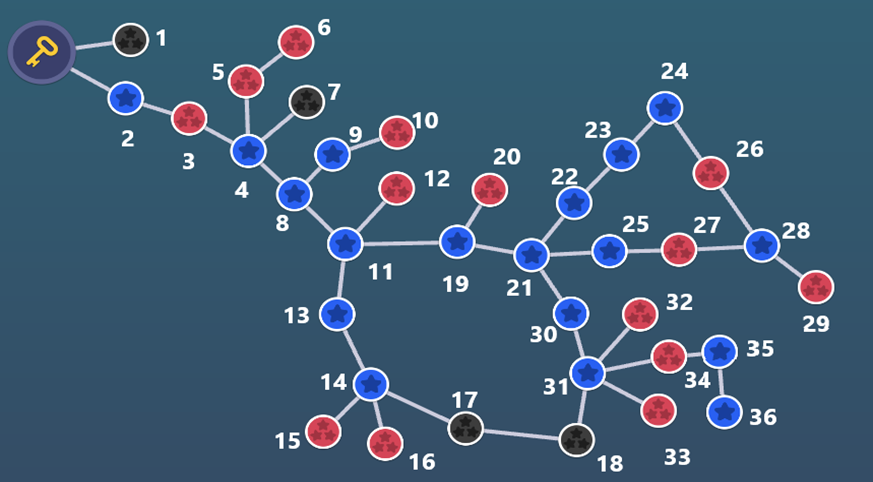
\includegraphics[width=9cm]{pictures/mathematic_angles_et_constructions}
\end{center}


\id{Tracer un triangle et une hauteur}

\defn{Une \emph{hauteur d'un triangle} est une droite qui passe par un sommet du triangle et qui est perpendiculaire au côté opposé à ce sommet.
}
\id{Tracer les autres hauteurs}

\rem{Les hauteurs d'un triangle se coupent en un point (sont concourantes).
Ce point est appelé l'\uline{orthocentre du triangle}.
}


%\arrow Ex. 33, 34 p.162 (T5) \datei{Bicher/T5/T5_p.162.jpg} \\
%\arrow Ex. 47 p.163 \datei{Bicher/T5/T5_p.163.jpg} \\
%\arrow Ex. 28, 31, 38 p.162 \\
%\arrow Ex. 45, 46 p.163



\section{La médiane}
\addexo{Pour chacun des triangles suivants, la droite $(AD)$ coupe les triangles en deux autres triangles.
Compare les surfaces des deux nouveaux triangles et explique la construction de la droite $(AD)$ à l'aide des sommets $A$, $B$ et $C$ seulement.
\begin{center}
\begin{tikzpicture}
	\draw[color=gro,dash pattern=on 1pt off 1pt, xstep=.5cm,ystep=.5cm] (-.2,-.2) grid (3.2,2.2);
	\draw (0,0)node[left]{$B$}
				--node[below](D){$D$} (3,0)node[right]{$C$}
				-- (1.5,2)node[above](A){$A$}
				--cycle;
	\draw[red] (A) --(D);
\end{tikzpicture}
\begin{tikzpicture}[scale=.7]
	\draw[color=gro,dash pattern=on 1pt off 1pt, xstep=1cm,ystep=1cm] (-.2,-2.2) grid (3.2,2.2);
	\draw (3,2)node[right]{$B$}
				--node[right](D){$D$} (3,-2)node[right]{$C$}
				-- (0,0)node[left](A){$A$}
				--cycle;
	\draw[red] (A) --(D);
\end{tikzpicture}
\begin{tikzpicture}[scale=.7]
	\draw[color=gro,dash pattern=on 1pt off 1pt, xstep=.5cm,ystep=.5cm] (-.2,.2) grid (2.2,-4.2);
	\draw (0,-4)node[left]{$B$}
				--node[below right](D){$D$} (2,0)node[right]{$C$}
				-- (0,0)node[above](A){$A$}
				--cycle;
	\draw[red] (0,0) --(1,-2);
	\draw[blue!20] (1,0) --(1,-2) --(0,-2);
\end{tikzpicture}
\begin{tikzpicture}[scale=.8]
	\draw[color=gro,dash pattern=on 1pt off 1pt, xstep=.5cm,ystep=.5cm] (-.2,-.2) grid (4.2,3.2);
	\draw (0,0)node[left]{$B$}
				--node[below](D){$D$} (4,1)node[right]{$C$}
				-- (1,3)node[above](A){$A$}
				--cycle;
	\draw[red] (1,3) --(2,.5);
\end{tikzpicture}
\end{center}
%\begin{center}
%\definecolor{qqzzqq}{rgb}{0.,0.6,0.}
%\definecolor{ttttff}{rgb}{0.2,0.2,1.}
%\definecolor{ffqqqq}{rgb}{1.,0.,0.}
%\definecolor{qqqqff}{rgb}{0.,0.,1.}
%\definecolor{cqcqcq}{rgb}{0.7529411764705882,0.7529411764705882,0.7529411764705882}
%\begin{tikzpicture}[scale=.6,line cap=round,line join=round,>=triangle 45,x=1.0cm,y=1.0cm]
%	\draw [color=cqcqcq,dash pattern=on 1pt off 1pt, xstep=1.0cm,ystep=1.0cm] (0.4204876451923835,0.5616892144800908) grid (5.579050674208538,5.660730362392205);
%	\clip(0.4204876451923835,0) rectangle (5.579050674208538,5.660730362392205);
%	\fill[color=ttttff,fill=ttttff,fill opacity=0.1] (5.,1.) -- (3.,5.) -- (3.,1.) -- cycle;
%	\fill[color=qqzzqq,fill=qqzzqq,fill opacity=0.1] (3.,1.) -- (3.,5.) -- (1.,1.) -- cycle;
%	\draw [color=ffqqqq] (3.,0.5616892144800908) -- (3.,5.660730362392205);
%	\draw [color=ttttff] (5.,1.)-- (3.,5.);
%	\draw [color=ttttff] (3.,5.)-- (3.,1.);
%	\draw [color=ttttff] (3.,1.)-- (5.,1.);
%	\draw [color=qqzzqq] (3.,1.)-- (3.,5.);
%	\draw [color=qqzzqq] (3.,5.)-- (1.,1.);
%	\draw [color=qqzzqq] (1.,1.)-- (3.,1.);
%	\draw [fill=qqqqff] (3.,5.) circle (1.5pt);
%	\draw[color=qqqqff] (3.1386535489432035,5.283758448733333) node {$A$};
%	\draw [fill=qqqqff] (1.,1.) circle (1.5pt);
%	\draw[color=qqqqff] (0.7974595588512564,1.256111160693803) node {$B$};
%	\draw [fill=qqqqff] (5.,1.) circle (1.5pt);
%	\draw[color=qqqqff] (5.142556879445633,1.2759517877284803) node {$C$};
%	\draw [fill=ffqqqq] (3.,1.) circle (1.5pt);
%	\draw[color=ffqqqq] (2.7,1) node[below] {$D$};
%	\draw[color=ffqqqq] (3.2180160570819134,8.835230687940603) node {$d$};
%\end{tikzpicture}
%\hspace{.25cm}
%\definecolor{qqzzqq}{rgb}{0.,0.6,0.}
%\definecolor{ttttff}{rgb}{0.2,0.2,1.}
%\definecolor{ffqqqq}{rgb}{1.,0.,0.}
%\definecolor{qqqqff}{rgb}{0.,0.,1.}
%\definecolor{cqcqcq}{rgb}{0.7529411764705882,0.7529411764705882,0.7529411764705882}
%\begin{tikzpicture}[scale=.6,line cap=round,line join=round,>=triangle 45,x=1.0cm,y=1.0cm]
%	\draw [color=cqcqcq,dash pattern=on 1pt off 1pt, xstep=1.0cm,ystep=1.0cm] (0.5593720344351262,0.5815298415147683) grid (5.777456944555313,3.498102015612359);
%	\clip(0.5593720344351262,0.5815298415147683) rectangle (5.777456944555313,3.498102015612359);
%	\fill[color=ttttff,fill=ttttff,fill opacity=0.1] (5.,3.) -- (1.,2.) -- (5.,2.) -- cycle;
%	\fill[color=qqzzqq,fill=qqzzqq,fill opacity=0.1] (5.,2.) -- (1.,2.) -- (5.,1.) -- cycle;
%	\draw [color=ffqqqq,domain=0.5593720344351262:5.777456944555313] plot(\x,{(--8.-0.*\x)/4.});
%	\draw [color=ttttff] (5.,3.)-- (1.,2.);
%	\draw [color=ttttff] (1.,2.)-- (5.,2.);
%	\draw [color=ttttff] (5.,2.)-- (5.,3.);
%	\draw [color=qqzzqq] (5.,2.)-- (1.,2.);
%	\draw [color=qqzzqq] (1.,2.)-- (5.,1.);
%	\draw [color=qqzzqq] (5.,1.)-- (5.,2.);
%	\draw [fill=qqqqff] (1.,2.) circle (1.5pt);
%	\draw[color=qqqqff] (0.9561845751286765,2.3076643935317094) node {$A$};
%	\draw [fill=qqqqff] (5.,1.) circle (1.5pt);
%	\draw[color=qqqqff] (5.182238133514987,1.2362705336591253) node {$B$};
%	\draw [fill=qqqqff] (5.,3.) circle (1.5pt);
%	\draw[color=qqqqff] (5.142556879445633,3.2798551182309064) node {$C$};
%	\draw [fill=ffqqqq] (5.,2.) circle (1.5pt);
%	\draw[color=ffqqqq] (5.221919387584343,1.83148934469945) node {$D$};
%	\draw[color=ffqqqq] (-5.035684789343934,2.327505020566387) node {$d$};
%\end{tikzpicture}
%\end{center}
%%
%\begin{center}
%\definecolor{qqzzqq}{rgb}{0.,0.6,0.}
%\definecolor{ttttff}{rgb}{0.2,0.2,1.}
%\definecolor{ffqqqq}{rgb}{1.,0.,0.}
%\definecolor{qqqqff}{rgb}{0.,0.,1.}
%\definecolor{cqcqcq}{rgb}{0.7529411764705882,0.7529411764705882,0.7529411764705882}
%\begin{tikzpicture}[scale=.6,line cap=round,line join=round,>=triangle 45,x=1.0cm,y=1.0cm]
%	\draw [color=cqcqcq,dash pattern=on 1pt off 1pt, xstep=1.0cm,ystep=1.0cm] (1.392678369891582,0.5220079604107358) grid (6.551241398907736,3.6568270318897786);
%	\clip(1.392678369891582,0.5220079604107358) rectangle (6.551241398907736,3.6568270318897786);
%	\fill[color=ttttff,fill=ttttff,fill opacity=0.1] (6.,1.) -- (3.,3.) -- (4.,1.) -- cycle;
%	\fill[color=qqzzqq,fill=qqzzqq,fill opacity=0.1] (4.,1.) -- (3.,3.) -- (2.,1.) -- cycle;
%	\draw [color=ffqqqq,domain=1.392678369891582:6.551241398907736] plot(\x,{(--9.-2.*\x)/1.});
%	\draw [color=ttttff] (6.,1.)-- (3.,3.);
%	\draw [color=ttttff] (3.,3.)-- (4.,1.);
%	\draw [color=ttttff] (4.,1.)-- (6.,1.);
%	\draw [color=qqzzqq] (4.,1.)-- (3.,3.);
%	\draw [color=qqzzqq] (3.,3.)-- (2.,1.);
%	\draw [color=qqzzqq] (2.,1.)-- (4.,1.);
%	\draw [fill=qqqqff] (3.,3.) circle (1.5pt);
%	\draw[color=qqqqff] (3.1386535489432035,3.2798551182309064) node {$A$};
%	\draw [fill=qqqqff] (2.,1.) circle (1.5pt);
%	\draw[color=qqqqff] (1.8093315376198098,1.256111160693803) node {$B$};
%	\draw [fill=qqqqff] (6.,1.) circle (1.5pt);
%	\draw[color=qqqqff] (6.134588231179508,1.2759517877284803) node {$C$};
%	\draw [fill=ffqqqq] (4.,1.) circle (1.5pt);
%	\draw[color=ffqqqq] (3.733872359983529,0.7997767388962207) node {$D$};
%	\draw[color=ffqqqq] (0.32128451001899594,8.835230687940603) node {$d$};
%\end{tikzpicture}
%\hspace{.25cm}
%\definecolor{qqzzqq}{rgb}{0.,0.6,0.}
%\definecolor{ttttff}{rgb}{0.2,0.2,1.}
%\definecolor{ffqqqq}{rgb}{1.,0.,0.}
%\definecolor{qqqqff}{rgb}{0.,0.,1.}
%\definecolor{cqcqcq}{rgb}{0.7529411764705882,0.7529411764705882,0.7529411764705882}
%\begin{tikzpicture}[scale=.6,line cap=round,line join=round,>=triangle 45,x=1.0cm,y=1.0cm]
%	\draw [color=cqcqcq,dash pattern=on 1pt off 1pt, xstep=1.0cm,ystep=1.0cm] (1.352997115822227,0.28392043599460604) grid (6.590922652977091,3.676667658924456);
%	\clip(1.352997115822227,0.28392043599460604) rectangle (6.590922652977091,3.676667658924456);
%	\fill[color=ttttff,fill=ttttff,fill opacity=0.1] (6.,3.) -- (2.,3.) -- (4.,2.) -- cycle;
%	\fill[color=qqzzqq,fill=qqzzqq,fill opacity=0.1] (4.,2.) -- (2.,3.) -- (2.,1.) -- cycle;
%	\draw [color=ffqqqq,domain=1.352997115822227:6.590922652977091] plot(\x,{(--8.-1.*\x)/2.});
%	\draw [color=ttttff] (6.,3.)-- (2.,3.);
%	\draw [color=ttttff] (2.,3.)-- (4.,2.);
%	\draw [color=ttttff] (4.,2.)-- (6.,3.);
%	\draw [color=qqzzqq] (4.,2.)-- (2.,3.);
%	\draw [color=qqzzqq] (2.,3.)-- (2.,1.);
%	\draw [color=qqzzqq] (2.,1.)-- (4.,2.);
%	\draw [fill=qqqqff] (2.,3.) circle (1.5pt);
%	\draw[color=qqqqff] (1.9680565538972299,3.3195363723002616) node {$A$};
%	\draw [fill=qqqqff] (2.,1.) circle (1.5pt);
%	\draw[color=qqqqff] (1.6307658943077121,0.978342382208318) node {$B$};
%	\draw [fill=qqqqff] (6.,3.) circle (1.5pt);
%	\draw[color=qqqqff] (6.134588231179508,3.2798551182309064) node {$C$};
%	\draw [fill=ffqqqq] (4.,2.) circle (1.5pt);
%	\draw[color=ffqqqq] (4.2100474088157895,1.83148934469945) node {$D$};
%	\draw[color=ffqqqq] (-5.035684789343934,6.335311681571239) node {$d$};
%\end{tikzpicture}
%\end{center}
}{-}

\defn{Une \emph{médiane d'un triangle} passe par un sommet et par le milieu du côté opposé à ce sommet.
}

\prop{Une médiane partage le triangle en deux surfaces de même aire.
}

\id{Tracer un triangle avec ces 3 médianes.}


\prop{Le point d'intersection des médianes d'un triangle est le centre de gravité de ce triangle. \\
C'est le \og point d'équilibre\fg{} de ce triangle.
}

\addexo{Construire le triangle $\Delta ABC$ tel que 
$$ \widehat{A}=70\degres\; AB=5\, cm\; BC=6\, cm. $$
Puis, construire la médiane issue de $B$.
}{-}

\addexo{Construire un triangle rectangle ainsi que ses trois médianes.
}{-}





\section{L'inégalité triangulaire}
Mathematic:
\begin{enumerate}[label=$\rightarrow$]
	\item 2, 3: vocabulaire,
	\item 28, 29 module angles et constructions,
	\item 22,24,24 fir constructioun CCC, CAC, ACA.
\end{enumerate}
	


%%%% Aal Versioun firum avancé/base
%Introduction: Quel chemin est le plus vite? Le chemin direct ou la déviation?
%
%\prop[Inégalité triangulaire]{Soient $A, B$ et $C$ trois points. Alors
%$$ AC \leq AB+BC. $$
%}
%
%\defn{Un triangle $ABC$ est \emph{isocèle en $A$} ssi ${\green A}B = {\green A}C$.
%\definecolor{zzttqq}{rgb}{0.6,0.2,0}
%\definecolor{qqqqff}{rgb}{0,0,1}
%\definecolor{cqcqcq}{rgb}{0.75,0.75,0.75}
%\begin{center}
%\begin{tikzpicture}[line cap=round,line join=round,>=triangle 45,x=1.0cm,y=1.0cm]
%	\clip(-1.48,0.78) rectangle (2.58,3.5);
%	\fill[color=zzttqq,fill=zzttqq,fill opacity=0.1] (-1,2) -- (2,3) -- (2,1) -- cycle;
%	\draw [color=zzttqq] (-1,2)-- (2,3);
%	\draw [color=zzttqq] (0.44,2.57) -- (0.5,2.4);
%	\draw [color=zzttqq] (0.5,2.6) -- (0.56,2.43);
%	\draw [color=zzttqq] (2,3)-- (2,1);
%	\draw [color=zzttqq] (2,1)-- (-1,2);
%	\draw [color=zzttqq] (0.5,1.4) -- (0.56,1.57);
%	\draw [color=zzttqq] (0.44,1.43) -- (0.5,1.6);
%	\fill [color=qqqqff] (-1,2) circle (1.5pt);
%	\draw[color=qqqqff] (-1.22,1.86) node {$A$};
%	\fill [color=qqqqff] (2,3) circle (1.5pt);
%	\draw[color=qqqqff] (2.16,3.28) node {$B$};
%	\fill [color=qqqqff] (2,1) circle (1.5pt);
%	\draw[color=qqqqff] (2.3,1.0) node {$C$};
%\end{tikzpicture}
%\end{center}
%}
%

%\arrow Ex. 19, 21, 23 p.161 (T5) \\
%\arrow Ex. 57 p.164 \datei{Bicher/T5/T5_p.164.jpg} \\
%\arrow Ex. 64, 67, 68, 69 p.165 \datei{Bicher/T5/T5_p.165.jpg} \\
%\arrow Ex. 70, 74 p.166 \datei{Bicher/T5/T5_p.166.jpg} \\



\section{La médiatrice et la bissectrice}
Mathematic: items 13-18 module angles et constructions.

\id{Wann si déi éischt Stonn am Mathematic gemaacht hunn, mindestens items 13 an 14, dann an der nächser Stonn folgende Résumé opschreiwen.
}

\ret{La \textbf{médiatrice d'un segment}:
\begin{enumerate}[label=$\rightarrow$]
	\item passe perpendiculairement par le milieu de ce segment.
	\item est l'ensemble des les points qui sont équidistants des extrémités du segment.
\end{enumerate}
La \textbf{bissectrice d'un angle}:
\begin{enumerate}[label=$\rightarrow$]
	\item partage cet angle en deux angles de même amplitude.
	\item est l'ensemble des points qui sont équidistants des côtés de cet angle.
\end{enumerate}
}

%\defn{La \textbf{médiatrice d'un segment} passe perpendiculairement par le milieu de ce segment.}
%
%\id{Dreieck mat de médiatrices zeechnen.}
%
%\prop{La médiatrice est l'ensemble de tous les points qui sont à égale distance des extrémités du segment.
%}

\addexo{Construire un triangle quelconque $ABC$.
\begin{enumerate}
	\item Où sont situés les points qui sont équidistants des sommets $A$ et $B$?
	\item Construire l'ensemble de tous ces points.
	\item Où sont situés les points qui sont équidistants des sommets $B$ et $C$?
	\item Construire l'ensemble de tous ces points.
	\item Que peut-on dire du (des) point(s) d'intersection des deux ensembles ci-dessus par rapport aux trois sommets du triangle $ABC$?
\end{enumerate}
}{Conclusion: définition du centre du cercle circonscrit.
}

\defn{Le point d'intersection des médiatrices de deux (et donc aussi de trois) côtés d'un triangle est équidistant des trois sommets de ce triangle et appelé \textbf{centre du cercle circonscrit} à ce triangle.
}

%\addexo{Construire le triangle $\Delta MNP$ tel que 
%$$ \widehat{P}=130\degres\; MN=4\, cm\; MP=7\, cm. $$
%Puis, construire le centre du cercle circonscrit au $\Delta MNP$.
%}{-}
%
%\addexo{Construire un triangle rectangle ainsi que son centre du cercle circonscrit.
%}{-}



















%%% -------------------------------- EXERCICEN PRINTEN

\clearpage
\begin{exercices}
\foreach \x/\y in \exos
{\exo \x
% \ifnum\value{exo}=13 \columnbreak \fi
 }
\end{exercices} % 2-3 semaines

\chapter{Nombres rationnels}



Manuel: $\Delta 4^e$, p.47

\section{Rappels et vocabulaire}

La division de 2 par 5 peut être notée sous forme d'une fraction: $\frac{2}{5}$.
Toute fraction représente donc une division qu'on n'effectue pas.
Comme on ne peut pas diviser par 0, le dénominateur ne peut pas être 0:
p.ex. $\frac{1}{0}$ n'existe pas!

$$ \frac{2}{4} = \frac{1}{2} $$

\attention Le trait de la fraction s'écrit toujours à la même hauteur que le signe d'égalité!

\begin{enumerate}[label=$\triangleright$]
 \item Si on divise le N et le D d'une fraction par le même nombre, alors la fraction est \uline{simplifiée} par ce nombre:
 $$ \dfrac{10}{15}=\dfrac{2}{3} $$
  \item \attention Si le numérateur est une somme ou une différence, alors on ne peut pas simplifier!
    $$ \frac{6+2}{4} = \frac{8}{4}=2 $$
    On doit avoir un seul nombre ou un produit (multiplication!):
    $$ \dfrac{8}{2}= \dfrac{2\cdot 4}{2}=\dfrac{4}{1}=4 $$
 
 \item Une fraction est appelée \uline{irréductible} si elle ne peut pas être simplifiée sans obtenir des nombres décimaux dans le N ou D.
 \id{noter des exemples}
 
 \item Si on multiplie le N et le D d'une fraction par le même nombre, alors la fraction est \uline{amplifiée} par ce nombre:
 $$ \dfrac{1}{2,7}=\dfrac{10}{27} $$
 
 \item Chaque entier peut être écrit sous forme fractionnaire:
 $$ 3=\frac{3}{1}; 5 = \dfrac{5}{1}; 13 = \dfrac{13}{1} $$
 
 \item Mais:
 $$ 1=\frac{1}{1} = \dfrac{2}{2} = \dfrac{3}{3} = ... $$

\end{enumerate}


 
\section{Fractions négatives}
$\frac{3}{5} > \frac{1}{5}$ mais $-\frac{3}{5} < -\frac{1}{5}$.
\id{Tracer une droite graduée verticale.}

De même: $\frac{1}{2} > \frac{1}{3}$ mais $-\frac{1}{2} < -\frac{1}{3}$.

\rem{Il est plus facile de classer les fractions si on réfléchit si elles sont comprises entre 0 et -1 ou bien plus petites que -1.}


$$\begin{array}{rlr}
 (-1):(+2) &=-0,5 &\text{écriture fractionnaire:} \frac{-1}{2}=-\frac{1}{2} \\
 (+1):(-2) &=-0,5 &\text{écriture fractionnaire:} \frac{1}{-2}=-\frac{1}{2} \\
 (-1):(-2) &=0,5  &\text{écriture fractionnaire:} \boxed{\frac{-1}{-2}=\frac{1}{2}}
\end{array}$$

Donc: 
$$ \boxed{\frac{-1}{2}=\frac{1}{-2} =-\frac{1}{2}} \quad \text{et} \quad \boxed{\frac{-3}{-5}=+\frac{3}{5}} $$
et en général:
\prop{
Quels que soient les nombres $a$ et $b$ ($b\overset{!}{\neq}0$):
$$ \dfrac{-a}{-b}=\dfrac{a}{b}  \qquad\text{et}\qquad  \dfrac{-a}{b}=\dfrac{a}{-b}=-\dfrac{a}{b} $$
}

\attention $-\frac{2+7}{3} = \frac{-(2+7)}{3}$. Il faut mettre des parenthèses, car le signe se rapporte à tous les termes du numérateur.


%Ex. 38,41,42,44,45,47 p.57 (T4) \datei{Bicher/T4/T4_p.057.jpg} \\
%Ex. 125 p.63 \datei{Bicher/T4/T4_p.063.jpg}



\subsection{Addition/Soustraction de fractions}
\stitle{Exemples}
\begin{enumerate}[label=\alph*)]
  \item $ \frac{1}{2}+\frac{1}{4} = $
  \item $ \frac{1}{3}-\frac{1}{4}= $
  \item $ \frac{3}{4} {\green +} \frac{{\red -}2}{5} =  \frac{15}{20} {\green +} \frac{{\red -}8}{20} = \frac{15{\green +}({\red -}20)}{7} = \frac{-5}{20} = -\frac{1}{4} $ 
  \item $ \frac{5}{20} + \frac{3}{15} +\frac{15}{25}= $
\end{enumerate}



\ret{1. On simplifie les fractions autant que possible avant de continuer, on avec tout autre calcul! \\
2. Addition/Soustraction $\rightarrow$ DC. \\
3. Le résultat doit être une fraction irréductible.
}

\addexo{Calculer.
\begin{multicols}{2}
\begin{enumerate}
  \item $ \dfrac{3}{4}+\dfrac{5}{6}-\dfrac{7}{12}= $
  \item $ \dfrac{23}{8}-\dfrac{5}{3}-\dfrac{4}{12}= $
  \item $ \dfrac{3}{2}+\dfrac{2}{3}-\dfrac{4}{5}= $
  \item $ \dfrac{11}{12}-\dfrac{3}{4}+\dfrac{2}{3}= $
  \item $ \dfrac{2}{3}-\dfrac{3}{4}+\dfrac{5}{2}= $
  \item $ \dfrac{5}{9}-\dfrac{6}{11}+\dfrac{2}{3}= $
\end{enumerate}
\end{multicols}
}{-}
\addexo{Calculer.
\begin{multicols}{2}
\begin{enumerate}
  \item $ \dfrac{3}{4}-\dfrac{1}{6}-\dfrac{1}{9}= $
  \item $ \dfrac{10}{15}+\dfrac{15}{12}-\dfrac{20}{18}= $
  \item $ \dfrac{3}{4}+\dfrac{7}{8}-\dfrac{4}{3}= $
  \item $ \dfrac{9}{10}-\dfrac{2}{15}+\dfrac{3}{5}= $
  \item $ \dfrac{98}{100}-\dfrac{196}{200}= $
  \item $ 1-\dfrac{8}{12}+\dfrac{18}{15}= $
\end{enumerate}
\end{multicols}
}{-}


%\arrow Ex. 60-65 p.58 (T4) \datei{Bicher/T4/T4_p.058.jpg} \\
%\arrow Ex. 108 p.61 \datei{Bicher/T4/T4_p.061.jpg} \\
%\arrow Ex. 114, 122 p.62 \datei{Bicher/T4/T4_p.062.jpg}


\addexo{Effectuer et réduire les expressions suivantes.
\begin{enumerate}
  \item $ \dfrac{3}{8}+\dfrac{35}{14}= $
  \item $ \dfrac{13}{3}-\dfrac{4}{9}= $
  \item $ \dfrac{13}{3}-\dfrac{4}{9}= $
  \item $ 0,625+\dfrac{7}{4}+\dfrac{33}{22}= $
  \item $ \dfrac{1}{2}+0,25+\dfrac{1}{3}-\dfrac{5}{6}= $
  \item $ \dfrac{11}{12}-0,75+\dfrac{10}{15}= $
\end{enumerate}
}{Enoncé: Effectuer et réduire les expressions suivantes.
\begin{enumerate}
  \item $ \dfrac{23}{8} $
  \item $ \dfrac{35}{9} $
  \item $ \dfrac{35}{9} $
  \item $ \dfrac{31}{8} $
  \item $ \dfrac{1}{4} $
  \item $ \dfrac{5}{6} $
\end{enumerate}
}

\addexo{Effectuer et réduire les expressions suivantes.
\begin{enumerate}
  \item $ \dfrac{14}{21}-\left( \dfrac{15}{20}+2,5-\dfrac{5}{12} \right)= $
  \item $ \dfrac{17}{12}-\dfrac{5^2}{18}= $
  \item $ \dfrac{10}{15}-\dfrac{15}{12}-\dfrac{20}{18}= $
  \item $ -\dfrac{11}{21}-\dfrac{18}{35}= $
  \item $ -\dfrac{66}{39}+\dfrac{4^3}{26}-\left(\dfrac{72}{52}-\dfrac{30}{65}\right)= $
  \item $ \dfrac{35}{10}-\left( \dfrac{39}{78}-\dfrac{12}{56} \right)= $
\end{enumerate}
}{Enoncé: Effectuer et réduire les expressions suivantes.
\begin{enumerate}
  \item $ -\dfrac{13}{6} $
  \item $ \dfrac{1}{36} $
  \item $ -\dfrac{61}{36} $
  \item $ -\dfrac{109}{105} $
  \item $ -\dfrac{2}{13} $
  \item $ \dfrac{45}{14} $
\end{enumerate}
}

\addexo{Effectuer et réduire les expressions suivantes.
\begin{enumerate}
  \item $ -\dfrac{21}{56}+\dfrac{32}{88}-\dfrac{17}{34} = $
  \item $ \dfrac{9}{14}-\dfrac{3}{21}= $
  \item $ -\dfrac{3}{5}-\dfrac{4}{7}-\dfrac{-2}{70}= $
  \item $ -\left(\dfrac{36}{96}+\dfrac{20}{55}\right) -\dfrac{22}{44} = $
  \item $ \dfrac{15}{45}-\dfrac{-12}{210}-\left(\dfrac{15}{75}+\dfrac{-9}{-35}\right)= $
  \item $ \dfrac{18}{20}-\dfrac{18}{135}+\dfrac{-18}{30}= $
\end{enumerate}
}{Enoncé: Effectuer et réduire les expressions suivantes.
\begin{enumerate}
  \item $ -\dfrac{45}{88} $
  \item $ \dfrac{1}{2} $
  \item $ -\dfrac{8}{7} $
  \item $ -\dfrac{109}{88} $
  \item $ -\dfrac{1}{15} $
  \item $ \dfrac{1}{6} $
\end{enumerate}
}



\subsection{Multiplication de fractions}
Un quart de deux tiers:
\begin{center}
	\definecolor{qqqqff}{rgb}{0,0,1}
	\definecolor{qqzzqq}{rgb}{0,0.6,0}
	\definecolor{cqcqcq}{rgb}{0.75,0.75,0.75}
	\begin{tikzpicture}[line cap=round,line join=round,>=triangle 45,x=1.0cm,y=1.0cm]
		\draw [color=cqcqcq,dash pattern=on 1pt off 1pt, xstep=1.0cm,ystep=1.0cm] (0.76,0.75) grid (5.31,4.38);
		\clip(0.76,0.75) rectangle (5.31,4.38);
		\fill[color=qqzzqq,fill=qqzzqq,fill opacity=0.1] (1,4) -- (5,4) -- (5,2) -- (1,2) -- cycle;
		\fill[color=qqqqff,fill=qqqqff,fill opacity=0.1] (1,2) -- (2,2) -- (2,4) -- (1,4) -- cycle;
		\draw (1,1)-- (5,1);
		\draw (5,1)-- (5,4);
		\draw (5,4)-- (1,4);
		\draw (1,4)-- (1,1);
		\draw [color=qqzzqq] (1,4)-- (5,4);
		\draw [color=qqzzqq] (5,4)-- (5,2);
		\draw [color=qqzzqq] (5,2)-- (1,2);
		\draw [color=qqzzqq] (1,2)-- (1,4);
		\draw [color=qqqqff] (1,2)-- (2,2);
		\draw [color=qqqqff] (2,2)-- (2,4);
		\draw [color=qqqqff] (2,4)-- (1,4);
		\draw [color=qqqqff] (1,4)-- (1,2);
	\end{tikzpicture}
\end{center}

$$  \dfrac{1}{4} \cdot \dfrac{2}{3} = \dfrac{1}{6} $$

\rem{On n'a pas besoin d'un DC!
}

%\arrow Ex. 68-77 p.59 (T4) \datei{Bicher/T4/T4_p.059.jpg}

Pour multiplier deux fractions, on:
\begin{enumerate}
	\item note d'abord le signe du produit,
	\item ensuite on simplifie chaque fois un N et un D.
\end{enumerate}

\subsection{Nombre inverse et division de fractions}
\id{pour 6Gb\,: inverse sans base négative.
}

Exemples:
\begin{multicols}{4}
\begin{enumerate}[label=\alph*)]
  \item $ 4 : \ldots = 2$
  \item $ 4 \cdot \ldots = 2 $
  \item $ 6 : \ldots = 1 $
  \item $ 6 \cdot \ldots = 1 $
  \item $ 8 : \ldots = 2 $
  \item $ 8 \cdot \ldots = 2 $
  \item $ 12 : \ldots = 4 $
  \item $ 12 \cdot \ldots = 4 $
\end{enumerate}
\end{multicols}

\prop{Diviser par un nombre $n$ revient à multiplier par son inverse $\frac{1}{n}$.
}

On appelle $\frac{1}{4}$ l'inverse de $4$ et $4$ l'inverse de $\frac{1}{4}$. \\
De même: $-\dfrac{1}{22}$ est l'inverse de $-22$.

\defn{\textbf{Deux nombres} sont \textbf{inverses} l'un de l'autre $\Leftrightarrow$ leur produit est égal à 1.
}

Exemples\,: 1; $\frac{1}{3}$; $-3$ $\frac{2}{3}$; $-\frac{3}{7}$.


%\arrow Ex. 78-83 p.59 (T4) \datei{Bicher/T4/T4_p.059.jpg} \\
%\arrow Ex. 84-98 p.60 \datei{Bicher/T4/T4_p.060.jpg}

Comme $0,25 = \frac{1}{4}$, on peut multiplier par 4 au lieu de diviser par 0,25. \\
($1:0,25 =4$ et donc $5:0,25 = 5  \cdot 4 = 20$.)

 % 3-4 semaines
%
%\chapter{Calcul littéral}

\section{Expressions littérales}
\noindent
Formule pour calculer le périmètre (=\og Umfang \fg) d'un carré:
$$ \mathcal{P}_{carré} = 4\cdot a $$
Et pour l'aire d'un carré :
$$ \mathcal{A}_{carré} = a\cdot a = a^2 $$
L'aire d'un triangle :
$$ \mathcal{A}_{\Delta} = \frac{b \cdot h}{2} $$
Ce sont des expressions littérales:

\defn{Une \textbf{expression littérale} est une expression dans laquelle un ou plusieurs nombres sont représentés par des lettres.
Ces lettres sont appelés \textbf{variables}.
}

Si on connait la longueur d'un côté du carré, alors on peut calculer son périmètre : \\
p. ex. si $a=5\, cm$, alors $\mathcal{P} = 4\cdot 5 = 20\, cm$.
C'est une valeur \textbf{numérique} ($\rightarrow$ nombre)! \\
Ou bien, si $x=12,5 m$ :...

\rem{Une seule expression littérale peut admettre une infinité de \textbf{valeurs numériques} différentes! \\
Les formules ci-dessus sont vraies pour toutes les valeurs (numériques) des lettres.
}

\addexo{Ecrire en fonction de $x$ la longueur $AB$.
\begin{enumerate}
\item \vspace{0pt}
\begin{center}
\definecolor{qqqqff}{rgb}{0,0,1}
\definecolor{cqcqcq}{rgb}{0.75,0.75,0.75}
\begin{tikzpicture}[line cap=round,line join=round,>=triangle 45,x=.9cm,y=.9cm]
	\draw (1,2)node[above] {$A$}-- (3,2)node[above] {$B$} --(7,2);
	\draw (2.02,2.08) -- (1.98,1.92);
	\draw (4.02,2.08) -- (3.98,1.92);
	\draw (6.02,2.08) -- (5.98,1.92);
	\draw[|-|] (1,1.6)--node[below] {$x$} (7,1.6);
	\fill [color=qqqqff] (1,2) circle (1.5pt);
	\fill [color=qqqqff] (3,2) circle (1.5pt);
	\fill [color=qqqqff] (5,2) circle (1.5pt);
	\fill [color=qqqqff] (7,2) circle (1.5pt);
\end{tikzpicture}
\end{center}
%
\item \phantom{x}
\begin{center}
\definecolor{qqqqff}{rgb}{0,0,1}
\definecolor{cqcqcq}{rgb}{0.75,0.75,0.75}
\begin{tikzpicture}[line cap=round,line join=round,>=triangle 45,x=.6cm,y=.6cm]
	\draw (1,2)node[above] {$A$}-- (3,2)node[above] {$B$} --(10,2);
	\draw (2.02,2.08) -- (1.98,1.92);
	\draw (4.02,2.08) -- (3.98,1.92);
	\draw (6.02,2.08) -- (5.98,1.92);
	\draw[color=black] (8.5,2) node[above] {$5$};
	\draw[|-|] (1,1.5)--node[below] {$x$} (10,1.5);
	\fill [color=qqqqff] (1,2) circle (1.5pt);
	\fill [color=qqqqff] (3,2) circle (1.5pt);
	\fill [color=qqqqff] (5,2) circle (1.5pt);
	\fill [color=qqqqff] (7,2) circle (1.5pt);
	\fill [color=qqqqff] (10,2) circle (1.5pt);
\end{tikzpicture}
\end{center}
\end{enumerate}
}{-}

\noindent
Ex. 25$-$27, 29, 30, 31, 35, 36 (écrire en fonction de $x$) p.130 (T5) \date{Bicher/T5/T5_p.130.jpg} \\
Ex. 50, 51 p.132 (égalités d'expressions littérales) \date{Bicher/T5/T5_p.132.jpg}

\defn{Deux \textbf{expressions littérales} sont \textbf{égales} si elles donnent le même résultat pour \uline{toutes les valeurs numériques} (!) qu'on peut donner aux lettres.
}



\section{La distributivité simple}
\id{ajouter distributivité double
}

\addexo{Dire pour chaque cas s'il s'agit d'une somme ou d'un produit. Indiquer aussi le nombe de termes ou de facteurs.
\begin{enumerate}
  \item $ 9+x $
  \item $ 9 \cdot x  $
  \item $ 3 \cdot (x+5) $
  \item $ 3 \cdot (x+5)-7$
  \item $ 3 \cdot x \cdot (x+11) $ 
\end{enumerate}
}{Enoncé : Dire pour chaque cas s'il s'agit d'une somme ou d'un produit. Indiquer aussi le nombe de termes ou de facteurs.
\begin{enumerate}
  \item $ 9+x $ est une somme de deux termes.
  \item $ 9 \cdot x  $ est un produit de deux facteurs.
  \item $ 3 \cdot (x+5) $ est un produi de deux facteurs.
  \item $ 3 \cdot (x+5)-7$ est une somme (différence) de deux termes.
  \item $ 3 \cdot x \cdot (x+11) $ est un produit de 3 facteurs.
\end{enumerate}
}

\addexo{Déterminer l'aire du grand rectangle (composé des deux petits) de deux façons différentes.
\begin{center}
\definecolor{qqwwcc}{rgb}{0,0.4,0}
\definecolor{ccqqqq}{rgb}{0.8,0,0}
\begin{tikzpicture}[line cap=round,line join=round,>=triangle 45,x=1.0cm,y=.6cm]
%	\clip(0.61,0) rectangle (7.5,4.4);
%	\fill[color=gro,fill opacity=0.1] (1,1)-- (3.5,1)-- (3.5,5)-- (1,5)-- cycle;
%	\draw[color=black!50] (1,1)-- (3.5,1)-- (3.5,5)-- (1,5)-- cycle;
%	\draw[color=black!80] (3.5,1)-- (5,1) -- (5,5) -- (3.5,5) -- cycle;
	\draw[|-|,color=ccqqqq] (1,.75) --node[below] {$a$} (3.5,.75);
	\draw[|-|,color=qqwwcc] (3.5,.5) -- node[below] {$b$} (5,.5);
	\draw[dashed] (3.5,1) --(3.5,5);
	\draw (1,1)-- (5,1)-- (5,5)-- (1,5)--node[left] {$k$} cycle;
%	\draw (3,-0.25) node {$a$ (2e cas)};	
\end{tikzpicture}
\end{center}
}{\noindent
Aire du grand rectangle: \\
Longueur $\cdot$ largeur = $k \cdot (a+b) $
\\
Autre méthode: \hspace{3.5cm}
$\mathcal{A}_{\text{rect. rouge}} + \mathcal{A}_{\text{rect. vert}} = k \cdot a + k \cdot b $
\\
Les deux expressions représentent la même aire et donc le même résultat!
$$ \boxed{k \cdot (a+b) = k \cdot a + k \cdot b} $$
}

\addexo{Déterminer l'aire du rectangle gris (à gauche) de deux manières différentes.
\begin{center}
\definecolor{qqwwcc}{rgb}{0,0.4,0}
\definecolor{ccqqqq}{rgb}{0.8,0,0}
\begin{tikzpicture}[line cap=round,line join=round,>=triangle 45,x=1.0cm,y=.6cm]
%	\clip(0.61,0) rectangle (7.5,4.4);
	\draw[color=gro,fill=gro,fill opacity=0.1] (1,1)-- (3.5,1)-- (3.5,5)-- (1,5)-- cycle;
	\draw[color=black!60] (3.5,1)-- (5,1) -- (5,5) -- (3.5,5) -- cycle;
%	\draw[|-|,color=ccqqqq] (1,.75) --node[below] {\red $a$} (3.5,.75);
	\draw[|-|,color=qqwwcc] (3.5,.6) --node[below] {$b$} (5,.6);
	\draw (1,1)-- (5,1)-- (5,5)-- (1,5)--node[left] {$k$} cycle;
	\draw[|-|] (1,-.2)--node[below] {$a$} (5,-.2);
\end{tikzpicture}
\end{center}
}{Les deux expressions représentent la même aire et donc le même résultat!
$$ \boxed{k \cdot (a-b) = k \cdot a - k \cdot b} $$
}

\prop[La distributivité simple]{Quels que soient les nombres relatifs $a, b$ et $k$, on a :
$$\begin{array}{rcll}
    \multicolumn{3}{c}{\underrightarrow{développer}}\\
    \tikz[baseline, anchor=base] \node (a) {$k \cdot (a+b)$};
    &=&
    \tikz[baseline, anchor=base] \node (c) {$k \cdot a + k \cdot b$}; \\
    \tikz[baseline, anchor=base] \node (b) {$k \cdot (a-b)$};
    &=&
    \tikz[baseline, anchor=base] \node (d) {$k \cdot a - k \cdot b$}; \\
    \multicolumn{3}{c}{\overleftarrow{factoriser}}
%    \\ \multicolumn{3}{c}{\text{(mise en évidence)}}
\end{array}$$
}\label{distr}
\begin{tikzpicture}[overlay]
  \draw[dotted] (a.north west) rectangle (b.south east);
  \node[anchor=east, text width=3.5cm] at (b.west) {produits \\ (formes factorisées)};
  \draw[dotted] (c.north west) rectangle (d.south east);
  \node[anchor=west, text width=4cm] at (d.east) {somme/différence (formes développées)};
  \node[anchor=south west, xshift=-.75cm] at (c.north) {(= transformer un produit en une somme)};
\end{tikzpicture}
distribuer = \og verteilen \fg, développer = transformer un produit en une somme.

\rem{Dans le calcul littéral, la distributivité simple est utilisé pour supprimer les parenthèses (si on veut effectuer) ou bien pour obtenir un produit ($\rightarrow$ équations, classe de 9e)
}

\rem{Dans le calcul numérique, on applique la DS pour rendre un calcul mental plus facile: \\
$$\begin{array}[t]{rl}
	 & 23 \cdot 103 \\
	=& 23 \cdot (100+3) \\
	=& 23 \cdot 100 + 23 \cdot 3 \\
	=& 2369
\end{array}
\text{\hspace{.5cm} ou encore \hspace{.5cm}}
\begin{array}[t]{rl}
	 & 23 \cdot 99 \\
	=& 23 \cdot (100-1) \\
	=& 23 \cdot 100 - 23 \cdot 1 \\
	=& 2277
\end{array}$$
}

\noindent
Ex. 48, 49 p.131 (T5) \date{Bicher/T5/T5_p.131.jpg}

\addexo{Recopier et compléter.
\begin{enumerate}[label=\alph*)]
  \item $ 7 \cdot (6 - \ldots) = \ldots - \ldots \cdot x $
  \item $ \ldots \cdot ( x \ldots y ) = k \cdot x - \ldots \cdot y $
  \item $ 3 \cdot ( a - \ldots) = \ldots - 3 \cdot b $
  \item $ \ldots \cdot ( x-\ldots) = 5 \cdot x - 10  $
  \item $ 6 \cdot (\ldots + c) = 18 + \ldots \cdot c $
  \item $ 2 \cdot (\ldots + a) = 6 + 2 \cdot \ldots $
\end{enumerate}
}{-}


\section{La mise en évidence d'un facteur commun}
\stitle{Problèmes}
\begin{enumerate}[label=\alph*)]
\item Calculer astucieusement (astucieux: \og pfiffig, schlau.\fg) $7 \cdot 985 + 7 \cdot 15$. \\
Réponse:
$\begin{array}[t]{rl}
 & \underbrace{{\red 7} \cdot 985}_{\text{1er terme}} + \underbrace{{\red 7} \cdot 15}_{\text{2e terme}} \\
= & {\red 7} \cdot (985+15) \\
= & \underbrace{7}_{\text{1er facteur}} \cdot \underbrace{1000}_{\text{2e facteur}} \\
= & 7000
\end{array}$
On a appliqué la distributivité pour mettre le facteur commun {\red 7} en évidence.

\item
$\begin{array}[t]{rll}
 & \underset{\text{2 termes}}{\underbrace{{\red 7} \cdot a} + \underbrace{{\red 7} \cdot b}} & $Le facteur commun {\red 7} a été mis en évidence.$ \\
= & \underset{\text{2 facteurs}}{\underbrace{{\red 7}} \cdot \underbrace{(a+b)}} &\leftarrow $ forme factorisée. (Les facteurs sont $7$ et $(a+b)$.)$
\end{array}$

\item
$\begin{array}[t]{rll}
 & {\red 3} \cdot a + {\red 3} \cdot b \\
= & {\red 3} \cdot (a+b) &\leftarrow $ forme factorisée. (Les facteurs sont $3$ et $(a+b)$.)$
\end{array}$

\item
$\begin{array}[t]{rll}
 & {\red k} \cdot a + {\red k} \cdot b &$Le facteur commun {\red k} est mis en évidence.$ \\
= & {\red k} \cdot (a+b) &\leftarrow $ forme factorisée. (Les facteurs sont $k$ et $(a-b)$.)$
\end{array}$
\end{enumerate}

C'est la distributivité simple:
$$\begin{array}{rcl}
    \multicolumn{3}{c}{\underrightarrow{développer}} \\
    \tikz[baseline] \node (a) { $k \cdot (a+b)$ };
     &=&
    \tikz[baseline] \node (c) { $k \cdot a + k \cdot b$ };  \\
    \tikz[baseline] \node (b) { $k \cdot (a-b)$ };
     &=& 
    \tikz[baseline] \node (d) { $k \cdot a - k \cdot b$ }; \\
    \multicolumn{3}{c}{\overleftarrow{factoriser}}
%    \\ \multicolumn{3}{c}{\text{(mise en évidence)}}
\end{array} $$
\tikz[overlay] \draw[dotted] (a.north west) rectangle (b.south east);
\tikz[overlay] \draw[dotted] (c.north west) rectangle (d.south east);
\tikz[overlay] \node[anchor=east] at (b.west) {formes factorisées $\rightarrow$ \,};
\tikz[overlay] \node[anchor=west] at (d.east) {\, $\leftarrow$ formes développées};
  

\noindent
Ex. 46,47 p.131 (T5) \date{Bicher/T5/T5_p.131.jpg}



\section{Réduire des expressions littérales}
Pour faciliter l'écriture, le signe de multiplication peut être omis si un des facteur est une variable (et donc une lettre):
$$ \begin{array}{rll}
  x \cdot y & = & xy \\
  3 \cdot a & = & 3a \\
  5 \cdot (x+y) &=& 5(x+y) \\
  a \cdot a &=& a^2 \\
  1 \cdot a &=& a \\
  x \cdot x \cdot x \cdot y \cdot y = x^3\cdot y^2 &=& x^3y^2
\end{array} $$

\rem{Si $x=3$, alors $2x= 2\cdot 3 \neq 23$.}
  
Comme  $a \cdot b = b \cdot a$, on a aussi:
$$ \boxed{ ab = ba} \text{ Commutativité de la multiplication} $$
De même: $ anna = aann= a^2n^2 $.

\addexo{Ecrire les expressions suivantes sous la forme la plus courte possible.
\begin{multicols}{2}
\begin{enumerate}
  \item $x \cdot y \cdot x = $
  \item $7 \cdot a \cdot 5 = $
  \item $3 \cdot b \cdot b = $
  \item $3 \cdot z \cdot x \cdot x = $
  \item $1 \cdot x = $
  \item $0 \cdot a = $
\end{enumerate}
\end{multicols}
}{-}


Considérons l'expression littérale $2\cdot y = 2y$: \\
$2$ est appelé coefficient numérique et \\
$y$ est la partie littérale de $2 \cdot y$; ce sont toutes les inconnues avec leurs exposants respectifs. \\
Par exemple:
$$\begin{array}{c|c|c|l}
  \textbf{expression littérale} & \textbf{coefficient} & \textbf{partie littérale} \\
  \cline{1-3}
  2 y & 2 & y &\tikz[baseline]{\node[xshift=-1cm] (1) {};} \\
  \cline{1-3}
  -4 a & -4 & a \\
  \cline{1-3}
  5 x y & 5 & x y &\tikz[baseline]{\node[anchor=west] (mid) {même partie littérale};}  \\
  \cline{1-3}
  9 x \cdot x = 9 x^2 & 9 & x \cdot x = x^2 \\
  \cline{1-3}
  7 y & 7 & y &\tikz[baseline]{\node[anchor=east] (2) {};} \\
  \cline{1-3}
  -42 l u x & -42 & l u x \\
  \cline{1-3}
  a\cdot 5 \cdot b=5ab & 5 & ab \\
  \cline{1-3}
\end{array}$$

\begin{tikzpicture}[overlay]
\path[<-] (1) edge[out=0, in=90] (mid);
\path[->] (mid) edge[out=270, in=0] (2);
\end{tikzpicture}

Tous les termes ayant une partie littérale identique sont appelés \textbf{termes semblables}. \\
Ce sont ici $2y$ et $7y$. Si on les ajoute, on obtient:
$$\begin{array}[t]{rll}
 & 2{\red y} +7{\red y} &$Le facteur commun {\red $y$} est mis en évidence.$ \\
=& (2+7) \cdot {\red y} \\
=& 9 \cdot y
\end{array}$$

\ret{Pour ajouter deux termes \uline{semblables}, il faut:
\begin{enumerate}[label=\arabic*.]
	\item ajouter les coefficients,
	\item garder la partie littérale.
\end{enumerate}
}

\rem{Cette méthode marche aussi avec des fractions: \\
$ \frac{1}{2}x +\frac{1}{2}x =.. $
ou bien
$ \frac{1}{3}x +\frac{3}{4}x =..$
\\
Mais $\frac{2}{3}x+\frac{2}{3}x^2$ ne peut pas être effectué! ($\neq$ termes semblables.)
}

\ret{Une multiplication peut toujours être effectuée, tandis qu'on a besoin d'une \textbf{même partie littérale pour ajouter} des termes:
\begin{enumerate}[label=\alph*)]
  \item $ 3m \cdot 6m = 6m^2 $
  \item $ 18m^2 \cdot 2m^2 = 36m^3 $
  \item $ 3m + 6m = 9m $
  \item $ 18m^2 + 2m^2 $ ne peut pas être réduit.
\end{enumerate}
}

\noindent
\arrow Ex. 55-57, 59, 62 p.132 (T5) \date{Bicher/T5/T5_p.132.jpg}



\section{Exercices supplémentaires}
\addexo{Développer les expressions suivantes.
\begin{enumerate}
	\item $ 2 \cdot (5+3x)= $
	\item $ 5 \cdot (a+x)= $
	\item $ 8 (4-y)= $
	\item $ x (5+3x)= $
	\item $ a (a-7b)= $
	\item $ c (y-6c)= $
\end{enumerate}
}{Enoncé: Développer les expressions suivantes.
\begin{enumerate}
	\item $ 6x+10 $
	\item $ 5a+5x $
	\item $ 32-8y $
	\item $ 5a+3x^2 $
	\item $ a^2 -7ab $
	\item $ cy-6c^2 $
\end{enumerate}
}
\addexo{Développer les expressions suivantes.
\begin{enumerate}
	\item $ 9 (15+32x)= $
	\item $ 5a (a+2x)= $
	\item $ 7c (5y-2c)= $
	\item $ 7x (6x-y)= $
	\item $ 11a (2+8ab)= $
	\item $ 9ab (a-7b)= $
\end{enumerate}
}{Enoncé: Développer les expressions suivantes.
\begin{enumerate}
	\item $ 135-288x $
	\item $ 5a^2+10ax $
	\item $ 35cy-14c^2 $
	\item $ 42x^2-7xy $
	\item $ 22y+88a^2b $
	\item $ 9a^2b-63ab^2 $
\end{enumerate}
}
\addexo{Développer les expressions suivantes.
\begin{enumerate}
	\item $ 2(a+b+2)= $
	\item $ 3(x-7+y)= $
	\item $ a(2x+a-b)= $
	\item $ x(2x-a-b)= $
	\item $ 2b(6-a+b)= $
	\item $ 7x(x+3y-5)= $
\end{enumerate}
}{Enoncé: Développer les expressions suivantes.
\begin{enumerate}
	\item $ 2a+2b+4 $
	\item $ 3x+3y-21 $
	\item $ a^2-ab+2ax $
	\item $ 2x^2-ax-bx $
	\item $ 2b^2 -2ab +12b $
	\item $ 7x^2+21xy-35x $
\end{enumerate}
}
\addexo{Développer les expressions suivantes.
\begin{enumerate}
	\item $ x (x-2y+5xy)= $
	\item $ 2x(y-5x+7b)= $
	\item $ 7a(5b-6a+7ab)= $
	\item $ 8z(9u-10zu-11u^2)= $
	\item $ 7s(-12t-6s)= $
	\item $ 12a(5a+7b-6c)= $
\end{enumerate}
}{Enoncé: Développer les expressions suivantes.
\begin{enumerate}
	\item $ x^2-2xy+5x^2y $
	\item $ 2xy-10x^2+14bx $
	\item $ 35ab-42a^2+49a^2b $
	\item $ 72zu-80z^2u-88zu^2 $
	\item $ -84st-42s^2 $
	\item $ 60a^2+84ab-72ac $
\end{enumerate}
}
\addexo{Développer les expressions suivantes.
\begin{enumerate}
	\item $ ab(5a-2b)= $
	\item $ xy(-x-8+y)= $
	\item $ xy(7x+6y-2xy)= $
	\item $ 4ax(5a-3b+7ax)= $
	\item $ 6an(an+ne)= $
	\item $ 9ab(-7a+5ab-4b)= $
\end{enumerate}
}{Enoncé: Développer les expressions suivantes.
\begin{enumerate}
	\item $ 5a^2b-2ab^2 $
	\item $ -x^2y-8xy+xy^2 $
	\item $ 7x^2y +6xy^2 -2x^2y^2 $
	\item $ 20a^2x -12abx +28a^2x^2 $
	\item $ 6a^2n^2 +6an^2e $
	\item $ -63a^2b +45a^2b^2 -36ab^2 $
\end{enumerate}
}
\addexo{Développer les expressions suivantes.
\begin{enumerate}
	\item $ -2(5+x)= $
	\item $ -7(6-8x)= $
	\item $ -x(3+x)= $
	\item $ -y(5-y)= $
	\item $ -(-a+b)= $
	\item $ -(a-b)= $
\end{enumerate}
}{Enoncé: Développer les expressions suivantes.
\begin{enumerate}
	\item $ -x-10 $
	\item $ 56x-42 $
	\item $ -x^2-3x $
	\item $ y^2-5y $
	\item $ a-b $
	\item $ b-a $
\end{enumerate}
}
\addexo{Développer les expressions suivantes.
\begin{enumerate}
	\item $ -2x(5+x)= $
	\item $ -7y(6-8x)= $
	\item $ -4y(3y+5x)= $
	\item $ -5y(5y-9)= $
	\item $ -12a(5a-b)= $
	\item $ -3b(8a-11b)= $
\end{enumerate}
}{Enoncé: Développer les expressions suivantes.
\begin{enumerate}
	\item $ -2x^2-10x $
	\item $ 56xy-42y $
	\item $ -12y^2-20xy $
	\item $ -25y^2+45 $
	\item $ -60a^2+12ab $
	\item $ 33b^2-24ab $
\end{enumerate}
}


\addexo{\textbf{Réduire} les expressions suivantes.
\begin{enumerate}
	\item $ 12 +6x -7x^2 -9x +4x^2 -15 = $
	\item $ a-2a-5+3a+7-4a-13 = $
	\item $ -5x+4y-12y+3x+y= $
	\item $ 9x^2-13x+x-5x^2-9x+17= $
	\item $ 8x-3+5y-2x+3y-11x= $
	\item $ 8a-3b+7+13a+17b-5a-25b-45= $
\end{enumerate}
}{Enoncé: Réduire les expressions suivantes.
\begin{enumerate}
	\item $ -3x^2-3x-3 $
	\item $ -2a-11 $
	\item $ -2x-7y $
	\item $ 4x^2-21x+17 $
	\item $ -5x+8y-3 $
	\item $ 16a-11b-38 $
\end{enumerate}
}
\addexo{Si possible, \textbf{réduire} les expressions suivantes.
\begin{enumerate}
	\item $ \frac{2}{4}x-\frac{5}{6}x= $
	\item $ \frac{25}{10}y+\frac{12}{18}y= $
	\item $ \frac{1}{9}x-\frac{1}{10}y= $
	\item $ \frac{27}{36}x^2 -\frac{16}{20}x +\frac{2}{11}x^2+\frac{4}{5}x= $
	\item $ \frac{1}{5}xy +\frac{4}{5}x-\frac{1}{6}y= $
	\item $ \frac{25}{50}x^2 -2x^2 +\frac{4}{5}x= $
\end{enumerate}
}{-}
\addexo{Développer et \textbf{réduire} les expressions suivantes.
\begin{enumerate}
	\item $ 19-3(x+2) = $
	\item $ 42 -x +3(2x+6) = $
	\item $ 3(9-y)-5(2+7y)= $
	\item $ 3(x-y+5)+5(2y-7x)= $
	\item $ 3(a-2b+c) +5(8+7b-a) = $
	\item $ -2\cdot(a-b+c) +3\cdot (-a+b+c) - 3 \cdot (b-c) = $
\end{enumerate}
}{Enoncé: Développer et \textbf{réduire} les expressions suivantes.
\begin{enumerate}
	\item $ -3x+13 $
	\item $ 5x+60 $
	\item $ -38y+17 $
	\item $ -32x+7y+15 $
	\item $ -2a+29b+3c+40 $
	\item $ -5a+2b+4c $
\end{enumerate}
}
\addexo{Développer et \textbf{réduire} les expressions suivantes.
\begin{enumerate}
	\item $ 45-20(x+2)-4x= $
	\item $ 12y-(5y+8)= $
	\item $ 10-3(a-5b+4)-(2b-3a)= $
	\item $ 11z-8z^2-(2z^2-15z+5)+4z-9= $
	\item $ 2(5a-7b+c+4)-3(5-a-4b-c)= $
	\item $ 3(x^2+x-2)-(3x^2+x+5)-x= $
\end{enumerate}
}{Enoncé: Développer et \textbf{réduire} les expressions suivantes.
\begin{enumerate}
	\item $ -24x+5 $
	\item $ 7y-8 $
	\item $ 3b+6 $
	\item $ -10z^2+30z-14 $
	\item $ 13a-2b+5c-7 $
	\item $ x-11 $
\end{enumerate}
}
\addexo{Développer et \textbf{réduire} les expressions suivantes.
\begin{enumerate}
	\item $ -6(2a-4b+1)+7(5-3a-b)= $
	\item $ 3x^2+2(1-x)-(2x-1)+x^2= $
	\item $ x+14y +4x +2(x-5y) = $
	\item $ 12a(3-7b+ax)= $
	\item $ -5(x-4y+9)+3(4-2x-8y)= $
	\item $ 3(2a-5b+8)-5(7-a+2b)= $
\end{enumerate}
}{Enoncé: Développer et \textbf{réduire} les expressions suivantes.
\begin{enumerate}
	\item $ -33a+17b+29 $
	\item $ 4x^2-4x+3 $
	\item $ 7x+4y $
	\item $ 12a^2x-84ab+36a $
	\item $ -11x-4y-33 $
	\item $ 11a-25b-11 $
\end{enumerate}
}
\addexo{Développer et \textbf{réduire} les expressions suivantes.
\begin{enumerate}
	\item $ 5-x(2x+7)+3\left(x^2-x+4\right)= $
	\item $ (5x-2)-(-7+x)-(3-2x)= $
	\item $ a(2a+b)-7a(a+2b)+3b(a-2b)= $
	\item $ -8a(b+c)+5b(2c-a)= $
	\item $ 3a-2 \cdot \left[ (a-b)-(5a+2b)\right]= $
	\item $ 19-2\left( x^2-3x+1 \right) -\left(5x^2-x+23 \right)= $
\end{enumerate}
}{Enoncé: Développer et \textbf{réduire} les expressions suivantes.
\begin{enumerate}
	\item $ x^2-10x+17 $
	\item $ 6x+2 $
	\item $ -5a^2-10ab-6b^2 $
	\item $ 10bc-13ab-8ac $
	\item $ 11a+6b $
	\item $ -7x^2+7x-6 $
\end{enumerate}
}
\addexo{Développer et \textbf{réduire} les expressions suivantes.
\begin{enumerate}
	\item $ 4(a-b)-3(2a+b)+9b= $
	\item $ 2c-7c(3c-5)+c(15-c)= $
	\item $ 12a(2b+7)+(3a-1)\cdot 15b-(74a+9ab)= $
	\item $ w(3w+4)-7-8w(-5-3w)-2(5-3w)= $
	\item $ 2(3y+7)+2y+5(6-y)-8(2y-3)= $
	\item $ 3a-2a^2-(-a^2+3+8a-5)+(5a-7-3a^2+6+2a)= $
\end{enumerate}
}{Enoncé: Développer et \textbf{réduire} les expressions suivantes.
\begin{enumerate}
	\item $ 2b-2a $
	\item $ -22c^2+52c $
	\item $ 60ab+10a-15b $
	\item $ 27w^2+50w-17 $
	\item $ -13y+68 $
	\item $ -4a^2+2a+1 $
\end{enumerate}
}
\addexo{Développer et \textbf{réduire} les expressions suivantes.
\begin{enumerate}
	\item $ 16x+6x\cdot x +3x (x-2)+(5x-3)\cdot x = $
	\item $ -12(4x-y-3)-8(7x+6y+3)+25+9x = $
	\item $ -(y-3x+2z)+(-x-z)-(3y+2x)= $
	\item $ x(x-3)-2x(1-x)= $
	\item $ 13a-4(2b+a-1)-(7a+5b-8)= $
	\item $ \left(4-3x^2+5x\right)$ $-\left(-2x+x^2\right)$ $-\left(2x^2-1\right) = $
\end{enumerate}
}{Enoncé: Développer et \textbf{réduire} les expressions suivantes.
\begin{enumerate}
	\item $ 14x^2+7x $
	\item $ -95x-36y+37 $
	\item $ -4y-32 $
	\item $ 3x^2-5x $
	\item $ 2a-13b+12 $
	\item $ -6x^2+7x+5 $
\end{enumerate}
}
\addexo{Développer et \textbf{réduire} les expressions suivantes.
\begin{enumerate}
	\item $ 2+5x(x-2)-3\left(15x-7x^2+11\right) = $
	\item $ 7x(2x-5)-4x(3-5x)= $
	\item $ -5(x-4y+9)+3(4-2x-8y)= $
	\item $ 6x\cdot 9 -7\cdot 6x^2+(-8x)\cdot(-3x)-9x \cdot 5 = $
	\item $ 3y^2+2(1-3y)-(7y-1)-5y^2= $
	\item $ -10(-10x+2)+4x(5x-8)= $
\end{enumerate}
}{Enoncé: Développer et \textbf{réduire} les expressions suivantes.
\begin{enumerate}
	\item $ 26x^2-55x-31 $
	\item $ 34x^2-47x $
	\item $ -11x-4y-33 $
	\item $ -18x^2+9x $
	\item $ -2y^2-13y+3 $
	\item $ 20x^2+68x-20 $
\end{enumerate}
}
\addexo{Développer et \textbf{réduire} les expressions suivantes.
\begin{enumerate}
	\item $ (-4x-8)\cdot 6+(10x-6)\cdot \left( -3x\right) = $
	\item $ 9x\cdot(2x-5)+ (7x-7)\cdot 7x - x\cdot(-5x+7) = $
	\item $ -9(-9x-4) -x(6x+5)+ 6(7x-8)- 6(-5x-8) = $
	\item $ -3x(6x-10) -9(-7x-8) +8(-x+6) -6(3x+7) = $
	\item $ 5x(8x-4) -4x(6x-6) -5(x+8) = $
	\item $ 9(-8x-7) -2x(7x-7)+ 7x(-7x+6) = $
\end{enumerate}
}{Enoncé: Développer et \textbf{réduire} les expressions suivantes.
\begin{enumerate}
	\item $ -38x^2-6x^2-48 $
	\item $ 62x^2-87x $
	\item $ -6x^2+148x+36 $
	\item $ -18x^2+67x+78 $
	\item $ 16x^2-x-40 $
	\item $ -63x^2-16x-63 $
\end{enumerate}
}
\addexo{Développer et \textbf{réduire} les expressions suivantes.
\begin{enumerate}
	\item $ 5x\left[10x-6-4(-3x-9)\right] = $
	\item $ 2(-2x+6) -4(-6x-3) = $
	\item $ (3x-10)\cdot \left( -2\right) -7x(10x-9)+ 5(-7x+8) = $
	\item $ -x(7x-8) -9x\left[-x+6-7x-(2x+7)\right] $
	\item $ 10(6x-5)- 7\left[5x-5-3(-10x+3)\right] = $
	\item $ 784x+5\,790xy+2\,024x^2-751\,544y = $
\end{enumerate}
}{Enoncé: Développer et \textbf{réduire} les expressions suivantes.
\begin{enumerate}
	\item $ 110x^2+150x $
	\item $ 20x+24 $
	\item $ -70x^2+22x+60 $
	\item $ 83x^2+17x $
	\item $ -185x+48 $
	\item Il n'y a pas de termes semblables qu'on peut ajouter.
\end{enumerate}
}

\addexo{Factoriser les expressions suivantes.
\begin{enumerate}
	\item $ 15x+5y= $
	\item $ 13ab-7b= $
	\item $ 18x-12y= $
	\item $ 33a-121b= $
	\item $ 23ab+b= $
	\item $ 3a^2-7ab= $
\end{enumerate}
}{Enoncé: Factoriser les expressions suivantes.
\begin{enumerate}
	\item $ 5(3x+y) $
	\item $ b(13a-7) $
	\item $ 6(3x-2y) $
	\item $ 11(3a-12b) $
	\item $ b(23a+1) $
	\item $ a(3a-7ab) $
\end{enumerate}
}
\addexo{Factoriser les expressions suivantes.
\begin{enumerate}
	\item $ 8a^2b-5b= $
	\item $ 17ac-6a^2c= $
	\item $ 4a-6a^2= $
	\item $ 9x-6x^2= $
	\item $ 27ax-18x= $
	\item $ 26a^2-169a= $
\end{enumerate}
}
{Enoncé: Factoriser les expressions suivantes.
\begin{enumerate}
	\item $ b(8a^2-5) $
	\item $ ac(17-6a) $
	\item $ 2a(2-3a) $
	\item $ 3x(3-2x) $
	\item $ 9x(3a-2) $
	\item $ 13a(2a-13) $
\end{enumerate}
}
\addexo{Si possible, factoriser les expressions suivantes. Sinon, expliquer pourquoi il est impossible de factoriser.
\begin{enumerate}
	\item $ 8x-16x^2= $
	\item $ 14xy-196y= $
	\item $ 5x-12y= $
	\item $ 9y+12xy^2= $
	\item $ 7x+xy+y= $
	\item $ 30xy+15x= $
\end{enumerate}
}{Enoncé: Si possible, factoriser les expressions suivantes. Sinon, expliquer pourquoi il est impossible de factoriser.
\begin{enumerate}
	\item $ 8x(1-2x) $
	\item $ 14y(x-14) $
	\item Les deux termes n'ont aucun facteur commun. Il est impossible de factoriser.
	\item $ 3y(3+4xy) $
	\item Les trois termes $7x$, $xy$ et $y$ n'ont aucun facteur commun. Il est impossible de factoriser.
	\item $ 15x(2y+1) $
\end{enumerate}
}
\addexo{Si possible, factoriser les expressions suivantes. Sinon, expliquer pourquoi il est impossible de factoriser.
\begin{enumerate}
	\item $ 2x^2+8xy= $
	\item $ 21y^2+14y= $
	\item $ 3a+6a^2+3= $
	\item $ 3xy-9x+10y= $
	\item $ 25x^2-5x+15xy= $
	\item $ 8xy+4y-16y^2= $
\end{enumerate}
}{Enoncé: Si possible, factoriser les expressions suivantes. Sinon, expliquer pourquoi il est impossible de factoriser.
\begin{enumerate}
	\item $ 2x(x+4y) $
	\item $ 7y(3y+2) $
	\item $ 3(a+2a^2+1) $
	\item Les trois termes $3xy$, $-9x$ et $10y$ n'ont aucun facteur commun. Il est impossible de factoriser.
	\item $ 5x(5x-1+3y) $
	\item $ 4y(2x+1-4y) $
\end{enumerate}
}









%%% -------------------------------- EXERCICEN PRINTEN

\clearpage
\begin{exercices}
\foreach \x/\y in \exos
{\exo \x
% \ifnum\value{exo}=10 \columnbreak \fi
% \ifnum\value{exo}=15 \columnbreak \fi
% \ifnum\value{exo}=20 \columnbreak \fi
% \ifnum\value{exo}=24 \columnbreak \fi
 }
\end{exercices}

\clearpage
\begin{solutions}
\foreach \x/\y in \exos
 {\sol \y
  }
\end{solutions}
 % 3-4 semaines
%
%%--- 3e trimestre
%\include{cours.6Gb.ch6.equations.1er.degre} % 3 semaines
%
%\chapter{Solides}
\id{Si gréisstendeels am Mathematic schaffe loossen,
just e puer Beispiller maachen fir ze üben an ze testen.
}

%cube, parallélépipède rectangle, prisme droit, cylindre

%Noter formules pour révision, ajouter quelques exercices. % 3 semaines
%
%\chapter{Représentation de données}
\id{Si gréisstendeels am Mathematic schaffe loossen,
just e puer Beispiller maachen fir ze üben an ze testen.
}

%cube, parallélépipède rectangle, prisme droit, cylindre

%Noter formules pour révision, ajouter quelques exercices. % 2 semaines
%
%\chapter{Probabilités}
dénombrements simples; diagramme en arbre, déf. exp. aléatoires; équiprobabilité;

%--- copy-paste vun der 9e
\section{Introduction et définitions}

\defn{Une \emph{expérience aléatoire} vérifie deux conditions:
\begin{enumerate}
	\item elle conduit à de s résultats qu'on est parfaitement capable de nommer,
	\item mais on ne sait pas lequel de ces résultats va se produire quand on réalise l'expérience.
\end{enumerate}
L'ensemble de tous les résultats est appelé \textbf{univers}, noté $\omega$ et
on appelle \textbf{événement}, tout sous-ensemble d'un univers.
}

Exemples d'expériences aléatoires:
\begin{enumerate}
\item Lancer une pièce de monnaie (2 résultats: pile et face.)
\item Lancement d'un dé équilibré.
\begin{itemize}
	\item L'univers représente tous les résultats possibles: $$ \Omega = \{ 1;2;3;4;5;6 \} $$
	\item Exemples d'événement: $A=$\og lancer un nombre pair\fg{} $=\{2; 4; 6\}$.
\end{itemize}
\item Tirer une carte parmi 32 ou 52. (32 ou 52 résultats)
\begin{itemize}
	\item L'univers: ... \id{c\oe ur, carreau, trèfle, pique}
	\item Exemple d'événement: ...
\end{itemize}
\end{enumerate}

\rem{Tous les résultats des univers des exemples d'expériences aléatoires ci-dessus sont \textbf{équiprobables}:
tous les éléments de l'univers ont la même probabilité.
}

\id{Si on a 6 résultat, alors chaque résultat a la probabilité $\frac{1}{6}$. (En cas d'équiprobabilité.)}

\id{Bsp ginn waat net éuiprobable ass.}


\addexo{On tire une carte parmi 32 (des valeurs de 7 à l'as et chaque valeur est représentée avec les 4 symboles).
\begin{enumerate}
 \item Noter l'univers de cette expérience.
 \item Noter quelques exemples d'événements.
 \item Déterminer la probabilité de ces événements.
\end{enumerate}
}{4 symboles: {\red c\oe ur, carreau}, {\blue trèfle, pique}.
}

\prop{La probabilité d'un événement peut être calculée à l'aide de la formule
$$ \dfrac{\text{cas favorables}}{\text{cas possibles}}, $$
à condition que tous les cas soient équiprobables. \\
La somme des probabilités de tous les résultats possibles (d'une expérience aléatoire) est égale à $1 (=100\%)$.
}

\addexo{On demande aux 25 élèves d'une classe combien ils ont de frères et s\oe ures. Voici les réponses:
\begin{center}
	0; 3; 1; 2; 4; 1; 2; 0; 1; 1; 2; 3; 0; \\
  1; 1; 5 ;2 ;1 ;0 ;2; 1; 0; 1; 0; 1.
\end{center}
On choisit au hasard un élève.
Déterminer la probabilité de tirer:
\begin{enumerate}
	\item un élève qui n'a aucun frère ou s\oe ur.
	\item un élève qui a un ou plus frères et s\oe urs.
	\item un élève qui a 2 frères et s\oe urs.
	\item un élève qui a 0; 1 ou 3 frères et s\oe urs.
\end{enumerate}
}{-}

\addexo{Dans un sac, il y a uniquement des boules bleues, des boules vertes et des boules rouges. On tire une boule au hasard. Léo a trouvé les résultats suivants:
\begin{itemize}
	\item $p($\og Obtenir une boule bleue\fg{})$=\frac{2}{5}$
	\item $p($\og Obtenir une boule verte\fg{})$=0,2$.
	\item $p($\og Obtenir une boule rouge\fg{})$=\frac{3}{9}$.
\end{itemize}
Est-ce possible?
}{-}

\addexo{On dispose d'un sac qui contient 10 boules:
\begin{itemize}
	\item 5 boules vertes,
	\item 3 boules rouges et 
	\item 1 boule blanche.
\end{itemize}
 On tire au hasard et on note la couleur de la boule. Déterminer la probabilité de chacun des événements suivants:
\begin{enumerate}
	\item $\ev{A}{Obtenir une boule rouge}$
	\item $\ev{B}{Ne pas obtenir une boule verte}$
	\item $\ev{C}{Obtenir une boule rouge ou une boule blanche}$
\end{enumerate}
}{-}

\addexo{Stéphane a le choix: tirer une boule dans le sac $A$ ou dans le sac $B$ sans voir ce qu'il tire. Il gagne s'il tire une boule \textbf{blanche}.
Quel sac doit-il choisir pour avoir le plus de chances de gagner?
\begin{center}
  \includegraphics[width=6cm]{pictures/prob_boules_bleues1.png}
\end{center}
}{-}

\addexo{Un sac contient 11 boules rouges, 6 boules noires et 3 boules jaunes. On tire une boule au hasard.
\begin{enumerate}
	\item Calculer la probabilité pour que cette boule soit rouge.
	\item Calculer la probabilité pour que cette boule soit noire ou jaune.
	\item On ajoute dans ce sac des boules bleues. Sachant que la probabilité de tirer une boule bleue est égale à un cinquième, déterminer le nombre de boules bleues qu'on a ajoutées.
\end{enumerate}
}{-}

\addexo{Dans une classe, le professeur choisit au hasard un élève qui sera l'arbitre du match de foot. La probabilité que ce soit un garçon est de deux tiers.
Calculer, si possible, la probabilité que ce soit une fille.
}{-}

\prop{La probabilité d'un événement est égale à 1 moins la probabilité de l'événement contraire:
$$ p(A) = 1- p \left(A^C \right) $$
}


\addexo{Chaque face d'un dé cubique est colorée. Il y a trois couleurs possibles: le jaune, le rouge et le blanc. On lance ce dé et on note la couleur de la face supérieure. On sait que la probabilité d'obtenir une face blanche est de deux tiers et que la probabilité d'obtenir une face rouge est d'un sixième.
\begin{enumerate}
	\item Déterminer la probabilité d'obtenir une face jaune.
	\item Déterminer le nombre de faces jaune.
\end{enumerate}
}{-}

\addexo{Qui a raison? Justifier.
\begin{center}
	\includegraphics[width=6cm]{pictures/prob_discussion.png}
\end{center}
}{-}

\addexo{Pierre a lancé 10 fois une pièce de monnaie et il a obtenu à chaque fois pile. Quelle est la probabilité d'obtenir aussi la 11e fois pile? Justifier.
}{-}

\defn{Soient $A$ et $B$ deux événements. Alors:
\begin{itemize}
	\item $A \cup B$ est l'événement qui a lieu si $A$ ou $B$ a lieu.
	\item $A \cap B$ est l'événement qui a lieu si $A$ et $B$ a lieu.
	\item $A^C$ ou $\overline{A}$ est l'événement qui a lieu si $A$ n'a pas lieu.
\end{itemize}
}


\addexo{Dans un stand de fête foraine, on fait tourner une roue, on attend qu'elle s'arrête et on note le numéro indiqué par la flèche.
\begin{center}
\includegraphics[width=5cm]{pictures/prob_roue1.png}
\end{center}
\begin{enumerate}
  \item Noter l'univers de cette expérience.
  \item Soit $\ev{A}{Obtenir un 3}$. Déterminer $p(A)$.
  \item Soit $\ev{B}{Obtenir un secteur blanc}$. Déterminer $p(B)$.
  \item Déterminer $p(A \cup B)$.
\end{enumerate}
}{-}


\addexo{On tire une carte d'un jeu de 52 cartes.
Déterminer la probabilité des événements suivants:
\begin{enumerate}[label=$\bullet$]
  \item A=\og \text{la carte tirée est une dame}\fg{}.
  \item B=\og\text{la carte tirée est un coeur}\fg{}.
  \item C=\og\text{la carte tirée n'est pas un coeur}\fg{}.
  \item D=\og\text{la carte tirée est le 5 de carreau}\fg{}.
  \item E=\og\text{la carte tirée est noire}\fg{}.
  \item $A \cup B$, ensuite $A\cap B$.
\end{enumerate}
}{-}




\section{L'arbre de choix}
\id{Op der 6Gb net um Programm
}
\id{Si 2 Würfelen gehei loossen, an d'somme vun deenen 2 opschreiwwen. Firwaat ass net alles d'selwecht wahrscheinlech?}

\addexo{On lance deux fois un dé à six faces.
\begin{enumerate}[label=$\bullet$]
	\item Noter tous les résultats possibles. Quel est le nombre de cas possibles?
	\item Soit $\ev{A}{La somme des yeux est 12.}$. \\ Déterminer $p(A)$.
	\item Soit $\ev{B}{La somme des yeux est 6.}$. \\ Déterminer $p(B)$.
	\item Soit $\ev{C}{La somme des yeux est supérieur à 9.}$. \\ Déterminer $p(C)$.
	\item Soit $\ev{D}{Obtenir au moins un 6.}$. \\ Déterminer $p(D)$.
	\item Soit $\ev{E}{Obtenir au moins un nombre pair.}$. \\ Déterminer $p(E)$.
\end{enumerate}
}{-}

\addexo{On lance trois pièces de monnaie. Déterminer:
\begin{enumerate}[label=$\bullet$]
  \item l'univers $\Omega$.
  \item les probabilités de chaque élément de l'univers.
  \item $p(\text{\og obtenir deux fois pile\fg{}})$
  \item $p(\text{\og obtenir deux fois face\fg{}})$
  \item $p(\text{\og obtenir au moins 2 fois face\fg{}})$
  \item $p(\text{\og obtenir au moins une fois face\fg{}})$
\end{enumerate}
}{$ \Omega = \left\lbrace (PPP); (PPF); .. \right\rbrace $.}


\rem{On peut grouper les entrées dans l'arbre de choix selon les besoins. \id{nombre pair/impair}}

\rem{On peut noter soit les cas possibles, soit les probabilités dans l'arbre de choix.
Si on veut éviter les fractions, alors on prend les cas possibles.
Mais ce n'est possible que si les résultats sont équiprobables.
}


\addexo{Au stand de foire, on propose le jeu suivant. Le joueur fait tourner la roue. Si l'aiguille indique un nombre pair, alors il tire un bille dans le sac. Si la bille est jaune, il gagne.
Déterminer la probabilité de gagner ce jeu.
\begin{center}
  \includegraphics[width=6cm]{pictures/prob_2etapes.png}
\end{center}
}{-}

\addexo{Un jeu consiste à tirer au hasard une boule du sac $A$. Si on tire une boule jaune, alors on a le droit de tirer une boule dans le sac $B$. On gagne alors un cadeau si on tire une boule bleue du sac $B$.
\begin{center}
	\includegraphics[width=6cm]{pictures/prob_2sacs.png}
\end{center}
Déterminer la probabilité de gagner ce jeu.
}{\id{evt prob. enzel rechnen an da multiplizéiren fir ze weien dat et daat selwecht resultat get}}

\addexo{Lors de la fête d'un club sportif, les organisateurs mettent en place un jeu pour gagner de l'argent pour le club avec la roue ci-dessous.
\begin{center}
  \includegraphics[width=3cm]{pictures/prob_roue2.png}
\end{center}
Il faut payer 2 \euro{} pour jouer le jeu.
Si on tire un 1, on ne gagne rien.
Si on tire un 2, on gagne 4 \euro.
Si on tire un 3, on gagne 5 \euro.
\begin{enumerate}
	\item Que gagne le jouer finalement s'il tire un 2? Et s'il tire un 3?
	\item Calculer la probabilité de perdre 2 \euro.
	\item Calculer la probabilité de gagner 2 \euro.	
	\item Calculer la probabilité de gagner 3 \euro.
	\item Est-il favorable de jouer ce jeu?
\end{enumerate}
}{L'organisateur n'a pas bien calculé.}


\addexo{Une urne contient sept boules indiscernables au toucher\,: quatre boules bleues et trois boules rouges.
\begin{enumerate}
	\item On tire successivement deux boules et on remet la boule tirée avant le deuxième tirage. Calculer les probabilités des événements suivants:
	\begin{enumerate}
		\item A=\og La première boule est bleue et la seconde boule est rouge. \fg{}
		\item B=\og Les deux boules ont la même couleur. \fg{}
	\end{enumerate}
	\item Reprendre la question précédente en supposant que le tirage s'effectue sans remise.
	\item Reprendre la question précédente en supposant que l'urne contienne aussi deux boules noires.
\end{enumerate}
}{-}



\clearpage
\begin{exercices}
\foreach \x/\y in \exos
{\exo \x
% \ifnum\value{exo}=4 \columnbreak \fi
% \ifnum\value{exo}=10 \columnbreak \fi
% \ifnum\value{exo}=17 \columnbreak \fi
% \ifnum\value{exo}=21 \columnbreak \fi
 }
\end{exercices}
 % 1-2 semaines




\end{document}